\documentclass[11pt]{article}
\usepackage[utf8]{inputenc}
\usepackage[
	letterpaper,
	left = .5in,
	right = .5in,
	top = 1in,
	bottom  = 1in
]{geometry}
\setlength{\columnsep}{.25in}
\usepackage{graphicx}
\usepackage{mathptmx}
\usepackage{float}
\usepackage[cmex10]{amsmath}
\usepackage{amsthm,amssymb}
\usepackage{url}
\urlstyle{same} 
\def\UrlBreaks{\do\/\do-}
\usepackage{breakurl}
\usepackage{fancybox}
\usepackage{breqn}
\usepackage{array}
\usepackage{colortbl}
\usepackage{booktabs}
\usepackage{caption}
\usepackage{subcaption}
%\usepackage{comment}
\usepackage[english]{babel}
\usepackage[acronym,nomain]{glossaries} % list of acronyms
%\usepackage{xurl}
\usepackage{multicol}
\usepackage{multirow}
\usepackage{mathptmx}
\usepackage{float}
\usepackage{lipsum}
%\usepackage{framed}
\usepackage[T1]{fontenc}
\usepackage[pdfpagelabels,pdfusetitle,colorlinks=false,pdfborder={0 0 0}]{hyperref}
%\usepackage{algorithm}
%\usepackage{algpseudocode}
%\usepackage{tabularx}
%\usepackage{wrapfig}
%\usepackage{enumitem}
\usepackage{paralist}

% draw a frame around given text
\newcommand{\framedtext}[1]{%
	\par%
	\noindent\fbox{%
		\parbox{\dimexpr\linewidth-2\fboxsep-2\fboxrule}{#1}%
	}%
}

\renewcommand{\arraystretch}{1.2}

\sloppy
\raggedbottom
\raggedcolumns

\setlength{\arrayrulewidth}{.5mm}

\newcolumntype{C}[1]{>{\centering\let\newline\\\arraybackslash\hspace{0pt}}m{#1-2\tabcolsep - \arrayrulewidth}}

\definecolor{LightCyan}{rgb}{0.88,1,1}
\definecolor{lightgray}{rgb}{.85, .85, .85}
\definecolor{whitesmoke}{rgb}{.95, .95, .95}



\usepackage[%
backend=bibtex,     % biber or bibtex
%style=authoryear,    % Alphabeticalsch
style=numeric-comp,  % numerical-compressed
sorting=none,        % no sorting
sortcites=true,      % some other example options ...
block=none,
indexing=false,
citereset=none,
isbn=true,
url=true,
doi=true,           % prints doi
natbib=true,         % if you need natbib functions
]{biblatex}
\addbibresource{./sources/sources.bib,}  % better than \bibliography

\title{A Quantitative Framework for Assessing Long-Trip Transportation Accessibility for Road Vehicles}
\author{Aaron I. Rabinowitz*, Vaishnavi Karanam, Radhika Gupta, Gil Tal**}
\date{}

\newacronym{ghg}{GHG}{Green-House Gas}
\newacronym{fe}{FE}{Fuel Economy}
\newacronym{ee}{EE}{Energy Economy}
\newacronym{epa}{EPA}{Environmental Protection Agency}
\newacronym{oem}{OEM}{Original Equipment Manufacturer}
\newacronym{ice}{ICE}{Internal Combustion Engine}
\newacronym{icv}{ICV}{Internal Combustion Vehicle}
\newacronym{icev}{ICEV}{Internal Combustion Engine Vehicle}
\newacronym{em}{EM}{Electric Motor}
\newacronym{hev}{HEV}{Hybrid Electric Vehicle}
\newacronym{ev}{EV}{Electric Vehicle}
\newacronym{phev}{PHEV}{Plug-in Hybrid Electric Vehicle}
\newacronym{lrphev}{LR-PHEV}{Long Range PHEV}
\newacronym{srphev}{SR-PHEV}{Short Range PHEV}
\newacronym{mhev}{MHEV}{Mild Hybrid Electric Vehicle}
\newacronym{pev}{PEV}{Plug-in Electric Vehicle}
\newacronym{bev}{BEV}{Battery Electric Vehicle}
\newacronym{cbev}{CBEV}{City BEV}
\newacronym{afv}{AFV}{Alternative Fuel Vehicle}
\newacronym{fcev}{FCEV}{Fuel Cell Electric Vehicle}
\newacronym{cav}{CAV}{Connected Autonomous Vehicle}
\newacronym{fc}{FC}{Fuel Consumption}
\newacronym{ec}{EC}{Energy Consumption}
\newacronym{dtto}{DTTO}{Discrete Time Trajectory Optimization}
\newacronym{udto}{UDTO}{Uniformly Discretized Trajectory Optimization}
\newacronym{sto}{STO}{Spline Trajectory Optimization}
\newacronym{rbed}{RBED}{Rules-Based Eco-Driving}
\newacronym{cidm}{CIDM}{Cooperative Intelligent Driver Model}
\newacronym{idm}{IDM}{Intelligent Driver Model}
\newacronym{soc}{SOC}{State of Charge}
\newacronym{ocp}{OCP}{Optimal Control Problem}
\newacronym{ttc}{TTC}{Time-To-Collision}
\newacronym{dp}{DP}{Dynamic Programming}
\newacronym{ga}{GA}{Genetic Algorithm}
\newacronym{sdm}{SDM}{Smart Driver Model}
\newacronym{v2i}{V2I}{Vehicle to Infrastructure}
\newacronym{v2v}{V2V}{Vehicle to Vehicle}
\newacronym{v2x}{V2X}{Vehicle to Everything}
\newacronym{hil}{HIL}{Hardware In Loop}
\newacronym{pso}{PSO}{Particle Swarm Optimization}
\newacronym{dt}{DT}{Direct Transcription}
\newacronym{oedt}{OEDT}{Optimal Eco-Driving Trace}
\newacronym{fods}{FODS}{Forward Object Detection System}
\newacronym{cas}{CAS}{Collision Aviodance System}
\newacronym{acc}{ACC}{Adaptive Cruise Control}
\newacronym{obu}{OBU}{On-Board Unit}
\newacronym{rsu}{RSU}{Road-Side Unit}
\newacronym{sae}{SAE}{Society of Automotive Engineers}
\newacronym{adas}{ADAS}{Advanced Driver Assistance System}
\newacronym{edc}{EDC}{Eco-Driving Control}
\newacronym{lv}{LV}{Lead Vehicle}
\newacronym{ss}{SS}{Segment Speeds}
\newacronym{hs}{HS}{Historical Speeds}
\newacronym{spat}{SPAT}{Signal Phase and Timing}
\newacronym{map}{MAP}{Positions of Subsequent Traffic Lights}
\newacronym{al2n}{AL2N}{Acceleration L\textsuperscript{2} Norm}
\newacronym{rpc}{RPC}{Road Power Cost}
\newacronym{bpc}{BPC}{Battery Power Cost}
\newacronym{fecc}{FECC}{Fitted Equivalent Consumption Cost}
\newacronym{ipopt}{IPOPT}{Interior-Point Optimization}
\newacronym{dtnlp}{DTNLP}{Discreet-Time Non-Linear Programming}
\newacronym{snlp}{SNLP}{Spline Non-Linear Programming}
\newacronym{sga}{SGA}{Spline Genetic Algorithm}
\newacronym{spso}{SPSO}{Spline Particle Swarm Optimization}
\newacronym{2sdp}{2SDP}{2 State Dynamic Programming}
\newacronym{aos}{AOS}{Approximate Optimal Spline}
\newacronym{pchip}{PCHIP}{Piecewise Cubic Hermitic Interpolation Polynomial}
\newacronym{nrel}{NREL}{National Renewable Energy Laboratory}
\newacronym{fastsim}{FASTSim}{Future Automotive Systems Technology Simulator}
\newacronym{mfei}{MFEI}{Mean Fuel Economy Improvement}
\newacronym{pas}{PAS}{Percent Acceptable Solutions}
\newacronym{mrt}{MRT}{Mean Run-Time}
\newacronym{mpc}{MPC}{Model Predictive Control}
\newacronym{adp}{ADP}{Approximate Dynamic Programming}
\newacronym{rl}{RL}{Reinforcement Learning}
\newacronym{mbrl}{MBRL}{Model Based Reinforcement Learning}
\newacronym{nlp}{NLP}{Non-Linear Programming}
\newacronym{nhtsa}{NHTSA}{National Highway Traffic Safety Administration}
\newacronym{aeb}{AEB}{Automatic Emergency Braking}
\newacronym{tsdc}{TSDC}{Transportation Secure Data Center}
\newacronym{anl}{ANL}{Argonne National Lab}
\newacronym{d3}{D\textsuperscript{3}}{Downloadable Dynamometer Database}
\newacronym{cd}{C\textsubscript{D}}{Coefficient of Drag}
\newacronym{crr}{C\textsubscript{RR}}{Coefficient of Rolling Resistance}
\newacronym{mape}{MAPE}{Mean Absolute Percentage Error}
\newacronym{evse}{EVSE}{Electric Vehicle Supply Equipment}
\newacronym{ld}{LD}{Light Duty}
\newacronym{md}{MD}{Medium Duty}
\newacronym{hd}{HD}{Heavy Duty}
\newacronym{mdhd}{MD/HD}{Medium Duty / Heavy Duty}
\newacronym{inrix}{INRIX}{}
\newacronym{epri}{EPRI}{Electric Power Research Institute}
\newacronym{nhts}{NHTS}{National Highway Transportation Survey}
\newacronym{usa}{USA}{United States of America}
\newacronym{sof}{SOF}{State of Fuel}
\newacronym{hc}{HC}{Home Charging}
\newacronym{bc}{BC}{Battery Capacity}
\newacronym{dcl}{DCL}{Destination Charger Likelihood}
\newacronym{ercr}{ERCR}{En-Route Charging Rate}
\newacronym{ercp}{ERCP}{En-Route Charging Penalty}
\newacronym{ftc}{FTC}{Fuel Tank Capacity}
\newacronym{ftp}{FTP}{Fuling Time Penalty}
\newacronym{psrc}{PSRC}{Puget Sound Regional Council}
\newacronym{bts}{BTS}{Bureau of Transportation Statistics}
\newacronym{happ}{HAPP}{Household Activity Pattern Problem}
\newacronym{chts}{CHTS}{California Houslehold Travel Survey}
\newacronym{dcfc}{DCFC}{DC Fast Charging}
\newacronym{liion}{Li-Ion}{Lithium-Ion}
\newacronym{lvl2}{LVL 2}{DC Level 2}
\newacronym{oems}{OEMS}{Optimal Energy Management Strategies}
\newacronym{poems}{POEMS}{Predictive Optimal Energy Management Strategies}
\newacronym{vpoems}{VP-OEMS}{Velocity Prediction enabled Optimal Energy Management Strategies}
\newacronym{gnss}{GNSS}{Global Navigational Satellite System}
\newacronym{obd2}{OBD-II}{On-Board Diagnostics II}
\newacronym{csu}{CSU}{Colorado State University}
\newacronym{wes}{WES}{Weight Efficiency Score}
\newacronym{gvwr}{GVWR}{Gross Vehicle Weight Rating}
\newacronym{fha}{FHA}{Federal Highway Administration}
\newacronym{vius}{VIUS}{Vehicle Inventory and Use Survey}
\newacronym{eod}{EOD}{End of Day}
\newacronym{osrm}{OSRM}{Open-Source Routing Machine}
\newacronym{vrp}{VRP}{Vehicle Routing Problem}
\newacronym{evrp}{EVRP}{Electric Vehicle Routing Problem}
\newacronym{tsp}{TSP}{Traveling Salesman Problem}
\newacronym{can}{CAN}{Controller Area Network}
\newacronym{lstm}{LSTM}{Long Short-Term Memory}
\newacronym{ann}{ANN}{Artificial Neural Network}
\newacronym{ml}{ML}{Machine Learning}
\newacronym{fcdp}{FC-DP}{Full Cycle Dynamic Programming}
\newacronym{ppmpc}{PP-MPC}{Perfect Prediction Model Predictive Control}
\newacronym{rpmpc}{RP-MPC}{Real Prediction Model Predictive Control}
\newacronym{cvmpc}{CV-MPC}{Constant Velocity Model Predictive Control}
\newacronym{mae}{MAE}{Mean Absolute Error}
\newacronym{fsmvrp}{FSMVRP}{Fleet Size and Mix Vehicle Routing Problem}
\newacronym{mcvrp}{MCVRP}{Monte-Carlo Vehicle Routing Problem}
\newacronym{ppf}{PPF}{Percent Point Function}
\newacronym{ccdng}{CCDNG}{Completely Connected Directional Network Graph}
\newacronym{sho}{SHO}{Spline Heuristic-Optimal}
\newacronym{npv}{NPV}{Net Present Value}
\newacronym{tco}{TCO}{Total Cost of Ownership}
\newacronym{mtk}{MTK}{Metric-Ton-Kilometer}
\newacronym{lco}{LCO}{Levelized Cost of Ownership}
\newacronym{lcod}{LCOD}{Levelized Cost of Driving}
\newacronym{sme}{SME}{Subject Matter Expert}
\newacronym{doe}{DOE}{Deparment of Energy}
\newacronym{vmt}{VMT}{Vehicle Miles Traveled}
\newacronym{dot}{DOT}{Department of Transportation}
\newacronym{ltl}{LTL}{Less Than Truckload}
\newacronym{lpcp}{LPCP}{Lost Payload Capacity Portion}
\newacronym{chaas}{ChaaS}{Charging as a Service}
\newacronym{tou}{TOU}{Time of Use}
\newacronym{ocs}{OCS}{Optimal Charging Strategy}
\newacronym{soe}{SOE}{State of Energy}
\newacronym{ltp}{LTP}{Lost Time Portion}
\newacronym{yd}{YD}{Yearly Distance}
\newacronym{dd}{DD}{Daily Distance}
\newacronym{vnr}{VNR}{Vehicle Nominal Range}
\newacronym{nyo}{NYO}{Number of Years of Ownership}
\newacronym{ap}{AP}{Age at Purchase}
\newacronym{dpm}{DPM}{Diesel Price Multiplier}
\newacronym{epm}{EPM}{Electricity Price Multiplier}
\newacronym{evsep}{EVSEP}{EVSE Premium}
\newacronym{pe}{PE}{Payload Exemption}
\newacronym{bpp}{BPP}{Battery Pack Pricing}
\newacronym{my}{MY}{Model Year}
\newacronym{ipfn}{IPFN}{Iterative Proportional Fitting with N dimensions}
\newacronym{dco}{DCO}{Discretized Control Optimization}
\newacronym{pto}{PTO}{Polynomial Trajectory Optimization}
\newacronym{slsqp}{SLSQP}{Sequential Least Squares Programming}
\newacronym{aer}{AER}{All Electric Range}
\newacronym{msrp}{MSRP}{Manufacturer Recommended Sales Price}
\newacronym{afdc}{AFDC}{Alternative Fuels Data Center}
\newacronym{uf}{UF}{Utility Factor}
\newacronym{hov}{HOV}{Hich Occupancy Vehicle}
\newacronym{lp}{LP}{Linear Problem}
\newacronym{qp}{QP}{Quadratic Problem}
\newacronym{sp}{SP}{Stochastic Problem}
\newacronym{slp}{S-LP}{Stochastic Linear Problem}
\newacronym{milp}{MILP}{Mixed Integer Linear Problem}
\newacronym{smilp}{S-MILP}{Stochastic Mixed Integer Linear Problem}
\newacronym{los}{LOS}{Level of Service}
\newacronym{v2s}{V2S}{Vehicle-to-Structure}
\newacronym{v2g}{V2G}{Vehicle-to-Grid}
\newacronym{gacm}{GACM}{Grid-Aware Charge Management}
\newacronym{iso}{ISO}{Independent System Operator}
\newacronym{dcopf}{DC-OPF}{DC Optimal Power Flow}
\newacronym{lmp}{LMP}{Location Marginal Price}
\newacronym{gcc}{GCC}{Giant Connected Component}
\newacronym{hjb}{HJB}{Hamilton-Jacobi-Bellman}
\newacronym{pdf}{PDF}{Probability Distribution Function}
\newacronym{scram}{SCRAM}{Stochastic Cost with Risk Allowance Minimization}
\newacronym{scramd}{SCRAM-D}{SCRAM-Dijkstra}
\newacronym{scramb}{SCRAM-B}{SCRAM-Bellman}
\newacronym{rsic}{RSIC}{Range-Sensitive Information Centrality}
\newacronym{rsbc}{RSBC}{Range-Sensitive Betweenness Centrality}
\newacronym{ras}{RAS}{Range Addition Station}

\makeglossaries

\begin{document}

\maketitle

\section*{Abstract}

I'll write this later - could maybe use some help

%A well designed transportation system provides sufficient access from origins to destinations to accommodate household and business demand in an economy.  Increasingly, climate action goals require that more transportation load be shifted to less \gls{ghg} intensive modes among which are \glspl{bev}. While \glspl{bev} use the same roads as \glspl{icev} they draw energy from a separate network of stations which neither as robust as nor coincident to the \gls{icev} fueling network, a consequence of the different current and historical economics of both. Insufficiency and unreliability of public DC \gls{evse} which is primarily used for charging on long itineraries mean that \gls{bev} drivers, depending on vehicle range and risk attitude, may opt for less direct paths with lower charging risk, opt for a more \gls{ghg} intensive mode, or abandon an itinerary. Holistically, the transportation system provides less access to \glspl{bev} for distant pairs. There is also stark disparity between \gls{bev} types. This project develops methods and tools to optimize deployment of future \gls{evse} to mitigate the issue. Methods herein are based on range and charging risk sensitive optimal routing between O/D pairs subject to the locations and usability rates of \gls{evse}. These methods and tools may be used by policymakers to directly evaluate the impact of proposed policies on \gls{bev} transportation access.
\medskip


\begin{multicols}{2}
	
\section{Introduction}

When discussing transportation networks, one must consider several linked and mutually supporting networks including road, rail, marine, and air infrastructure in addition to those energy and information networks which allow for vehicles to function. Multiple support systems are required for the efficient and economical operation of vehicles which underpins modern economies and standards of living. The various networks are coincident at a subset of nodes but, otherwise, may be operated in various manners by dissimilar stakeholders in service of divergent objectives. none of the related networks is a subset of any other but all share dependence relationships which may be asymmetrical.

The mode of vehicles in today's transportation sector, whether passenger or cargo oriented, are \glspl{icev} but a growing number of these vehicles are being supplanted by \glspl{pev}. This shift necessitates a re-alignment of the networks underpinning travel as the nodes of interaction between physical infrastructure and the energy system are incompatible between \glspl{icev} and \glspl{bev}. \glspl{icev} receive energy from a fuel distribution network which connects extraction operations to processing plants and ultimately to distribution stations. The fueling network is inherently inefficient due to constraints on the location of extraction sites, the economies of scale and access related to processing sites, and the requirement to expend fuel to transport fuel to end user locations which are widely distributed. It is, nevertheless, the case that this network has been subject to tremendous amounts of capital expenditure and operational optimization such that it's function and economic viability is ensured as long as extricable fuel supplies continue to be discovered and fuel-burning vehicles continue to be used.

\glspl{pev}, by contrast, draw energy from the electricity distribution network which also powers static loads such as those from buildings. Also the recipient of substantial and continuous investment, the power grid has been, historically, optimized to meet demand from buildings via the utilization of dispatchable resources including fuel-burning power plants. As the number of \glspl{pev} continues to rise, the load required to power these vehicles will become a greater portion of the overall load required. The interaction between vehicles and the power grid is heavily bound by constraints at coincident nodes and within their valency. Limitations exist on power transfer rates between the charger and battery as well as between the charger and power generation as a function of the distribution grid.

The most salient difference between the \gls{icev} fuel delivery network and the \gls{evse} network is at the interaction points. There are many more fueling stations in any given region of a developed country than public chargers. On the other hand, there are many more private charging locations than private fueling locations. \glspl{pev} are able to charge at low rates from many nodes including homes and buildings which are connected to the grid. Low rate charging is preferable for several reasons including lower costs per kWh and lower battery degradation. High rate charging is generally reserved for situations wherein charge time is relevant such as on itineraries whose distance is in excess of a vehicle's single charge range or for daily use by people unable to charge at home/work. The multifaceted nature of \gls{pev} charging contrasts to that of \gls{icev} fueling which takes lace at public access stations and at similar rates for the vast majority of fueling events. A significant portion of \gls{pev} users can accomplish most charging without relying on public-access stations and these are encourages to maintain this behavior. The multi-tiered "charging pyramid" dictates that fewer public-access fast charging stations can be supported for a given number of \glspl{pev} compared to fueling stations and \glspl{icev}.

As a result of the economic realities of charging stations, increases in network cardinality have, generally, been driven by incentives. The goal of these incentives is to create a network of public-access charging stations which is sufficiently ubiquitous and reliable that potential buyers will view \glspl{pev} as completely viable vehicles. A secondary goal would be to incentivise an efficient distribution of these stations such that profitable operations can be maintained after the subsidy period runs out. This document outlines methods of analysis for these networks which are fundamental and extensible and provide insights which can be used for further roll-out.

\section*{Transportation Accessibility}

Transportation accessibility has been studied as a tool for urban and regional planners since the middle of the 20\textsuperscript{th} century. Accessibility derives from the theory of population migration proposed by Ravenstein in 1885 \cite{Ravenstein_1885}. The movement of populations over a given time-scale can be analogized to Ohm's Law. In this analogy push and pull factors determine the "voltage" separation, traversal difficulty is the "resistance" and the resulting "current" is the flow. Human migration is subject to endogenous and nonlinear effects as flows lead to changes in their origin and destination locations as well as on the arc between. The field of transportation accessibility uses this framework to study regional efficiency considering both demand and impedance simultaneously. The accepted definition of transportation accessibility is the ease with which individuals can access relevant opportunities subject to the transportation system in the relevant area. Thus, accessibility is a framework which encompasses demand factors such as land use and temporal availability, impedance factors such as transportation system design, and universal factors such as personal preference \cite{Geurs_2004}. Literature provides four essential frameworks for computing access as surveyed in \cite{Handy_1997, Kwan_1998, Geurs_2004, Miller_2018, Handy_2020} and discussed below.

Much of the difference between methodologies is in scoping. Individuals are assumed to need or desire location-specific opportunities such as employment and physical retail. However, there may be several near-equivalents for any given opportunity type. The simplest methods for selecting opportunities are based on nearest proximity \cite{Wachs_1973, Vickerman_1974}. Proximity methods consider that a person has a level of access to a given need as determined by that person's proximity to the closest relevant opportunity. These methods do not account for heterogeneity within an opportunity category nor for the benefits of redundancy within an opportunity category. The inverse are isocost methods wherein a person is said to have access as determined by the number of opportunities available within a given isocost polygon. This method has the drawback of not considering the differences in arc traversal cost for \gls{od} pairs within the isocost region. These methods have been used widely \cite{Easa_1993} due to their transparency and computational lightness and form the basis for modern big-data methods such as the US DOE's Mobility Energy Productivity metric \cite{Hou_2019}.

Proximity and isocost methods are easy to compute because they treat redundancy arbitrarilys. In practice, equivalent and near-equivalent opportunities compete with one-another if sufficiently proximate or if the paths required to reach them overlap \cite{Stouffer_1940}. Gravity/entropy methods \cite{Noulas_2012, Jung_2008} address this shortcoming. These methods are so called as they concern the cumulative effect of opportunities for a given origin. Effects can accumulate on the basis of demand over proximity (gravity) or information content (entropy). Such methods were first formalized into a quantitative framework in 1959 \cite{Hansen_1959} as a generalization of previous methodology for quantifying the efficiency of urban land use. Gravity/entropy methods define accessibility as the intensity of the possibility for interaction. Implicit in the formulation of gravity/entropy methods is that every opportunity has some effect on every individual, even if negligible, and the effect of any one opportunity is determined by its network position.

Proximity and gravity/entropy methods rely on the assumption that traversal cost is the primary factor determining individuals decision to select one opportunity from among a set of similar entities. While this is certainly true if the difference in traversal cost is large enough it is not obvious what the threshold of disambiguation will be for a given individual or population. Researchers have proposed to use Discrete Choice Modeling \cite{Ben_Akiva_1985} to explain revealed choices wherein ease-of-access is merely one of several contributing factors in determining the utility of a given opportunity for a given individual \cite{Cevero_1995, Shen_1998, Karst_2003}.

Which method one chooses for an analysis should reflect the scope and purpose of that analysis. Definition of scope can be difficult and arbitrary and can lead to self-defeating policies in the worst cases \cite{Handy_1996}. This study is concerned with the effects of electrification on long-trip accessibility for road vehicle users. This scope simplifies opportunity selection. It is necessary that a transportation system provide for access between large population centers within a region of interest and to those in adjacent regions. This study is focused on non-routine regional travel rather than routine local travel as this is where supply infrastructure becomes important. It should be noted that the method is, nevertheless, valid for all travel scales. Said methodology is developed in the following section.

\section*{Methods}

The focus of this study is long-trip accessibility for road vehicles. The metric proposed reflects the ease with which a given individual, driving a given vehicle, can access the important locations in a region from one-another. It is assumed that travelers, when considering non-routine long trips have a specific destination in mind and would not consider nearly equivalent and/or equidistant locations as fungible. Rather, having determined to travel to a given location the traveler will then select a mode. Accessibility is a function of demand and impedance. Demand can be estimated by considering the relative attractiveness of given cities as a function of population, economy, or some other metric. Impedance can be quantified by calculating the mode and person specific lowest-cost-paths for all pairs of selected locations within the region and taking the average. Example costs which might be used are travel time and travel price.

A transportation accessibility metric should have land-use, transportation, temporal, and individual components \cite{Karst_2003}. The metric proposed contains all required components. The land-use within a region has two principle effects. First, for a multi-city region, peripheral cities should experience worse regional access than central cities. Second, geographically large and/or sparse regions should experience worse overall accessibility than compact regions. The transportation infrastructure determines the efficacy of various modes. Where only vehicular travel is concerned, the mode choice is reduced to vehicle choice. Vehicle specific infrastructure is not necessarily the same for all vehicles of a given fuel type but is necessarily different between fuel types creating effectively separate modes. The temporal component arises from the schedules of public transportation services and road traffic patterns. Finally the individual component is the traveler risk attitude and route cost weights.

\subsection*{Metric Definition}

Regional travel is often modeled using gravity models. Gravity models theorize that the attraction between two entities is in proportion to the general attractiveness of each and the intervening distance. The units of the resulting attraction have no physical meaning. A region where the sum or average attraction is higher will be a more integrated region. Being concerned with regional performance, this study proposes the Regional Gravity metric $G_R$. For region $R$ of $N$ nodes $O = \{O_1, O_2, \dots, O_N\}$ and a corresponding set of importance weights $W = \{W_0, W_1, \dots, W_N\}$, $G_R$ is computed as

\begin{equation}
	G_{R} = \frac{1}{N^2}\sum_{i = 0}^{N} \sum_{j = 0 }^{N} \frac{CW_iW_j}{Z_{ij}^2} \label{eq:regional_gravity}
\end{equation}

\noindent where $Z_{ij}$ is the cost of the optimal path from $O_i$ to $O_j$ and C is a constant tunable parameter. The Specific Regional Gravity $G_{R,i}$ at any node in region $R$ can be computed as

\begin{equation}
	G_{R,i} = \frac{1}{N}\sum_{j = 0 }^{N} \frac{CW_iW_j}{Z_{ij}^2} \label{eq:specific_regional_accessibility}
\end{equation}

for origin $O_i \in O$. Generally, $W$ will be the set of population masses for each location $M = \{M_0, M_1, \dots, M_N\}$. All else being equal, regions which are more populated/productive, more compact, and enjoy better transportation networks will experience higher $G_R$. This quantity will vary within the region. This study is primarily concerned with the transportation system which contributes directly to arc traversal cost rather than arc demand. Thus a second metric, Regional Impedance is defined as

\begin{equation}
	Z_{R} = \frac{1}{N^2}\sum_{i = 0}^{N} \sum_{j = 0 }^{N} Z_{ij} \label{eq:regional_impedance}
\end{equation}

for region $R$. Specific Regional Impedance $Z_{R,i}$ is defined as

\begin{equation}
	Z_{R,i} = \frac{1}{N}\sum_{j = 0 }^{N} Z_{ij} \label{eq:specific_regional_impedance}
\end{equation}

for a single origin. The Regional Impedance is the average cost of traversing an arc between nodes in a region. Any increase to $Z_R$ would result in a decrease to $G_R$.

\subsection*{Metric Computation}

Powered vehicles are range-limited due to the finite capacity of their \glspl{ess}. In order to traverse an \gls{od} arc whose energy requirement is greater than a vehicle's \gls{ess} capacity, the vehicle must stop at a supply station. In practical terms, the limit is defined by the vehicle's \gls{ess} capacity, starting \gls{soc}, desired finishing \gls{soc}, and the driver's low \gls{soc} tolerance. Because supply events add time to a trip, they will usually be minimized where possible \cite{Ge_2022}. For sufficiently long trips, where at least one supply event is necessary, computing the shortest-time path requires considering the time added during supply events and the time required to deviate to supply stations. For \glspl{icev}, supply events are brief and supply stations are ubiquitous in most areas of the developed world. Thus, conventional routing services often neglect supply considerations. For \glspl{bev}, supply events are relatively lengthy and DC supply stations are comparatively rare. Ignoring supply events when computing a shortest-time path for a \gls{bev} carries non-negligible risk of a lengthy stop or an out-of-charge event. For this reason, dedicated \gls{bev} routing services such as A Better Route Planner compute routes considering supply events.

All drivers deal with uncertainty and latency issues when computing an optimal route. Certain categories of disruption such as traffic, accidents, supply equipment functionality, and supply equipment local demand cannot be precisely known at the start of the trip. This uncertainty will cause different drivers to evaluate the same arc differently and may result in the selection of different routes. Compounding uncertainty is latency. Although a driver may have access to on the current state of roads and stations to be encountered in the future this may provide little information about conditions upon arrival. Without the ability to reserve a slot at a supply station, drivers cannot be certain of equipment availability until they physically arrive at the station. As such, drivers have to optimize an expectation of route costs when selecting routes. Such optimization may take the form of electing to take a longer ring highway to avoid city traffic, stopping for fuel more often in a sparsely populated area, sitting through a traffic jam rather than diverting, or any number of other strategies. This mental process is modeled via stochastic optimization.

\subsubsection*{Stochastic Optimal Routing}

The purpose of stochastic optimal routing is to find lowest-expected-cost paths from origin $i \in V$ to a set of destinations $D \in V$ on graph $G = \{V, E\}$. The output is tree $P$ containing the optimal-feasible paths from the origin to the selected destinations. The objective of routing on arc $(i,j)\ i, j \in V$ is

\begin{equation}
	\min_{U \in \overline{U}_{i,j}}\ \mathbb{E}[J(S_0, U)]
\end{equation}

where

\begin{equation}
	J(U) = \sum_{k = 0}^M \Phi_k(S_0, U)
\end{equation}

s.t.

\begin{gather}	
	b^k_l \leq \mathbb{E}\left[\int_0^t \Phi_k(S_0, U)dt\right] \leq b^k_u\\
	\mathbb{E}\left[\int_0^T \Phi_k(S_0, U)dt\right] \geq b^k_f\\
	t \in [0, T]\quad k = 1, 2, \dots, M
\end{gather}

\noindent where $T$ is the final value of time for a route, $S$ is the state vector of $M$ states, $S_0$ is the initial values of the states, $U$ is a path between $i$ and $j$, $\overline{U}_{i,j}$ is the set of possible paths between $i$, and $j$, $\Phi$ is the set of cost functions, $b^k_l$ and $b^k_u$ are the upper and lower bounds for state $k$ respectively, and $b^k_f$ is the final state minimum value for state $k$. $\mathbb{E}$ denotes an expectation. State vector $S$ is initialized and stored as vectors containing $N$ discreet variables. A distribution $D$ for a the state vector at any node and time-step can be computed from a histogram of the values. Routes are considered feasible if state expectations remain within set bounds. Comparison between routes is performed using cost expectation. the goal of the optimization is to find the optimal path $U_{ij}^*$ such that $J(U_{ij}^*)$ is equal to the global minimum cost $J_{ij}^*$ for each arc $(i,j)\ i,j\in V$.

For vehicle routing, common states are time, distance, price, number of stops, and remaining range. Limits are, often, placed on states and these may not be violated at any time. Limits may also be placed on the final value of a state. Time, distance, price, and number of stops are examples of metrics of minimization which may be used individually or in combination. Upper limits may be set on metrics of optimization in order to terminate the optimization when it is no longer possible to find a feasible route. Remaining range will, necessarily, be subject to upper and lower limits and may be subject to a final value limit (an example of this would be preserving enough range for a return trip). In this study, states are total trip time, driving time, and \gls{soc}.

The values of states are static at nodes and are changed in the process of traversing edges. Intuitively, if a vehicle has 50 km or remaining range at node $i$ and traverses edge $(i, j)$ of distance 20 km ($\Phi_d(i,j) = 20$) then it will arrive at node $j$ with 30 km of remaining range. If node $j$ contains a supply station then range can be added before progressing further. Adding range will cost time and money and should, therefore, be done sparingly. In order to progress from node $j$ to node $k$, the vehicle needs only sufficient range to avoid violating the associated lower bound, in this case 10 km. If $\Phi_d(j,k) \leq 20$ then no resupply is needed. If $\Phi_d(j,k) > 20$ then a resupply event is needed and should add only enough range to make $(j,k)$ feasible. Thus the cost of traversing $(j,k)$ depends on whether or not and how much resupply is needed. 

The extent to which range can be added via resupply is limited by the capacity of the vehicle's \gls{ess} and remaining range constraints. Certain edges will be infeasible regardless of supply as a result. In addition, supply will not be available at all nodes and the cost of supply is neither guaranteed to be homogeneous throughout a network nor to be linear with respect to range added.

The structure of the optimization process is as follows. First, a graph is created to represent the supply network and its interactions among itself and with origins and destinations of interest. All arcs which are feasible should be included as edges in this graph, including those directly between origins and destinations. This graph is described in the \gls{sng} subsection. Second, edge costs in terms of problem states are assigned using models which will be described in the Driver Model, Vehicle model, and Supply Station Model subsections. Third, stochastic optimization is performed using an optimal routing algorithm such as the Dijkstra or Bellman-Ford algorithm.

\subsubsection*{Supply Network Graph}

Supply networks effect routing both in structure and in the characteristics of individual stations. In this paper, the supply network refers to all stations which the vehicle can utilize.Supply networks ultimately consist of individual supply ports (chargers or fuel pumps) and serve geographically and temporally distributed demand. A network consisting of more than one port can develop redundancy either by concentrating ports in a single confined space "in-station" or via a more evenly distributed approach "between-station". In-station redundancy is simply the number of ports in a given station. Between-station redundancy is the number of ports in the set of stations which are sufficiently close as to be reinforcing. The distance that defines whether or not two stations are reinforcing varies between individuals and by a variety of factors. Network redundancy also varies by location with "thinner" and "thicker" coverage areas.

The physical connection between supply stations is provide by the road network. Without consideration of range, each station, origin, and destination is reachable from all others. The \gls{sng} is formed from these nodes. Edges are created for all origins and destinations based on shortest paths computed on the road map. Only the locations of and relationships between relevant nodes are necessary. The graph formed from the relevant nodes and their relationships is a reduced subgraph with a low number of nodes and relatively high edges-per-node and cycles-per-node ratios when compared ot the road map.

A reduced subgraph is defined as follows. For a graph $G = \{V, E\}$ where $V$ is the set of nodes and $E$ is the set of edges, a reduced subgraph $\hat{G} = \{\hat{V}, \hat{E}\}$ can be computed where $\hat{V} \subseteq V$ and $\hat{E} = \{P_{ij}\ \forall\ (i, j)\ \in\ \hat{E}\}$ is the set of shortest-paths between all nodes in $\hat{V}$. An example of a reduced subgraph is shown in Figure \ref{fig:reduced_subgraph}.

\begin{figure}[H]
	\centering
	\begin{subfigure}[t]{.5\linewidth}
		\centering\captionsetup{width = .8\linewidth}
		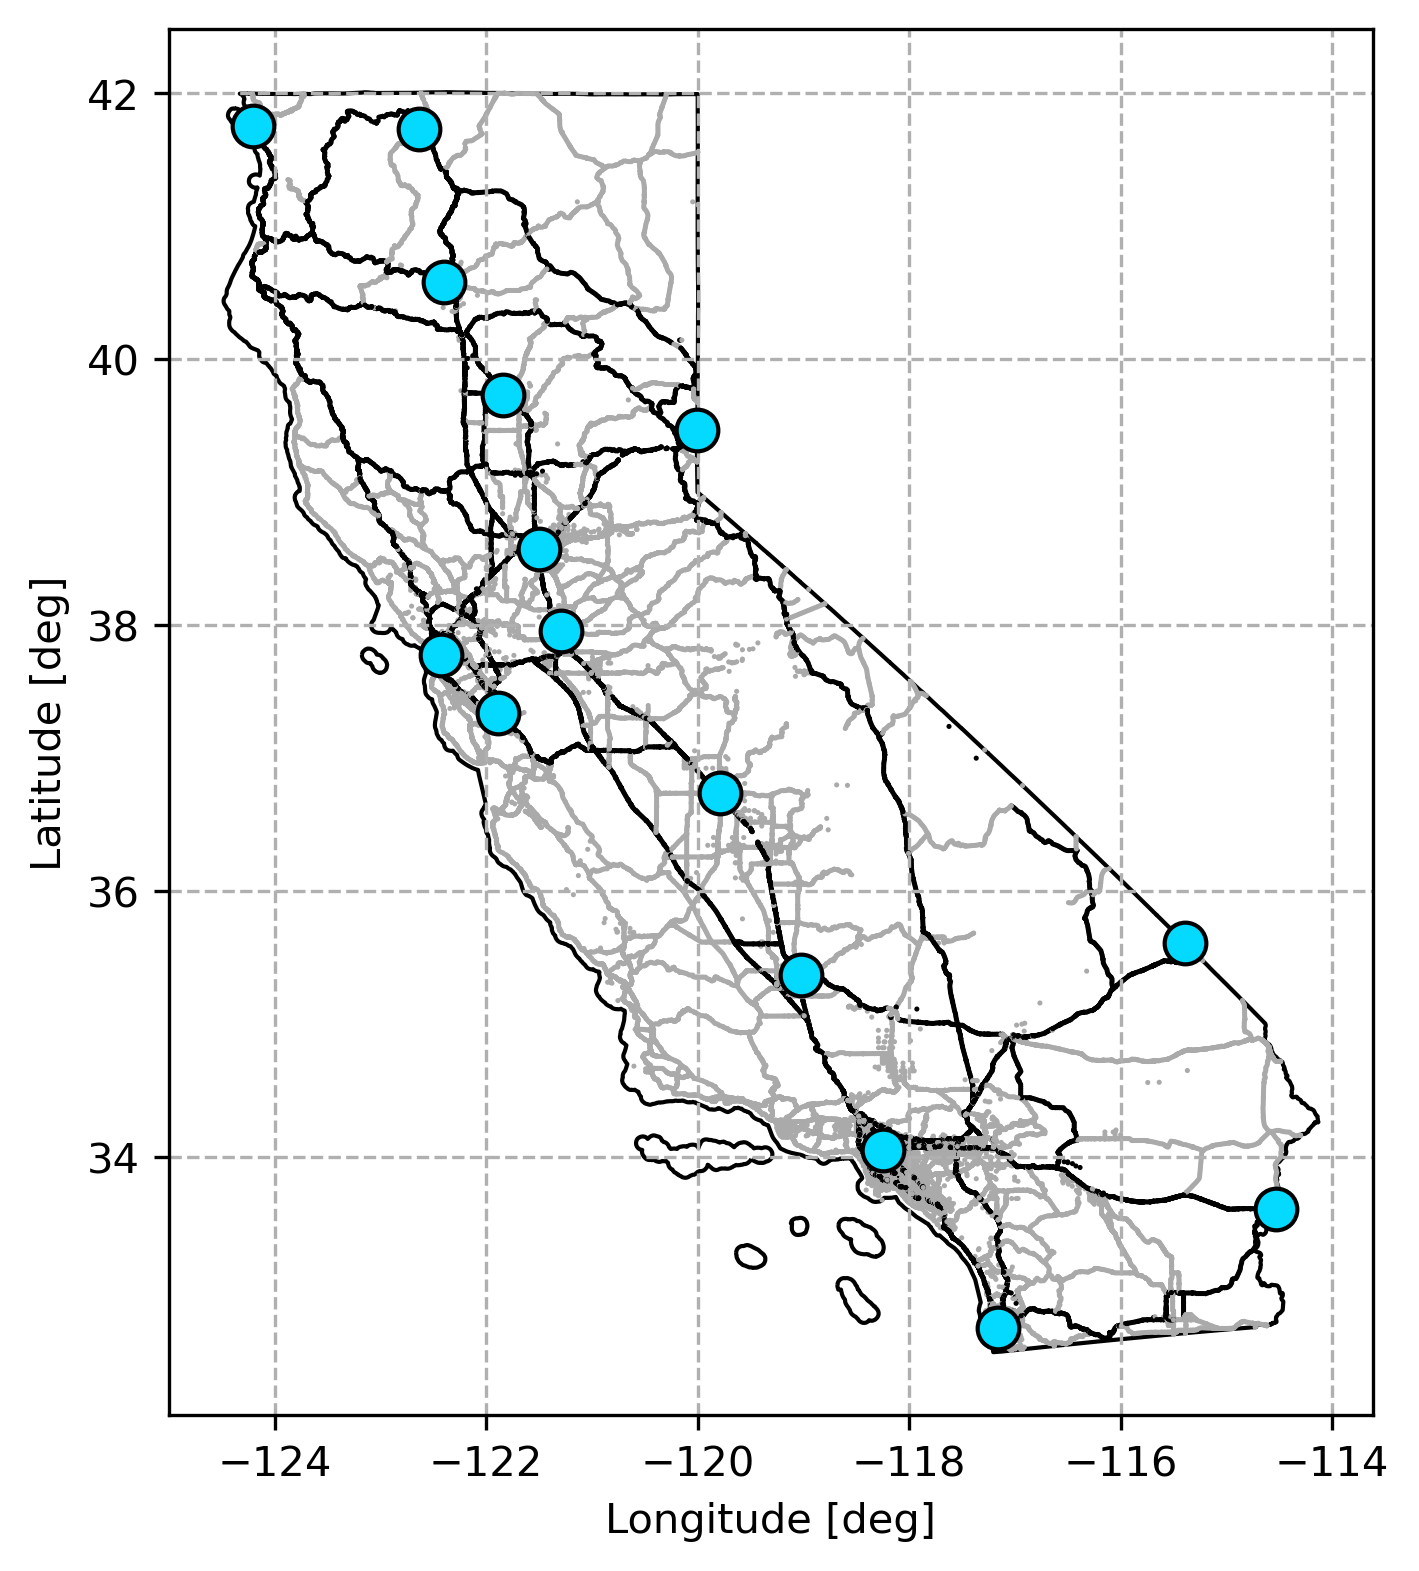
\includegraphics[width = \linewidth]{figs/full_graph.png}
	\end{subfigure}%
	\begin{subfigure}[t]{.5\linewidth}
		\centering\captionsetup{width = .8\linewidth}
		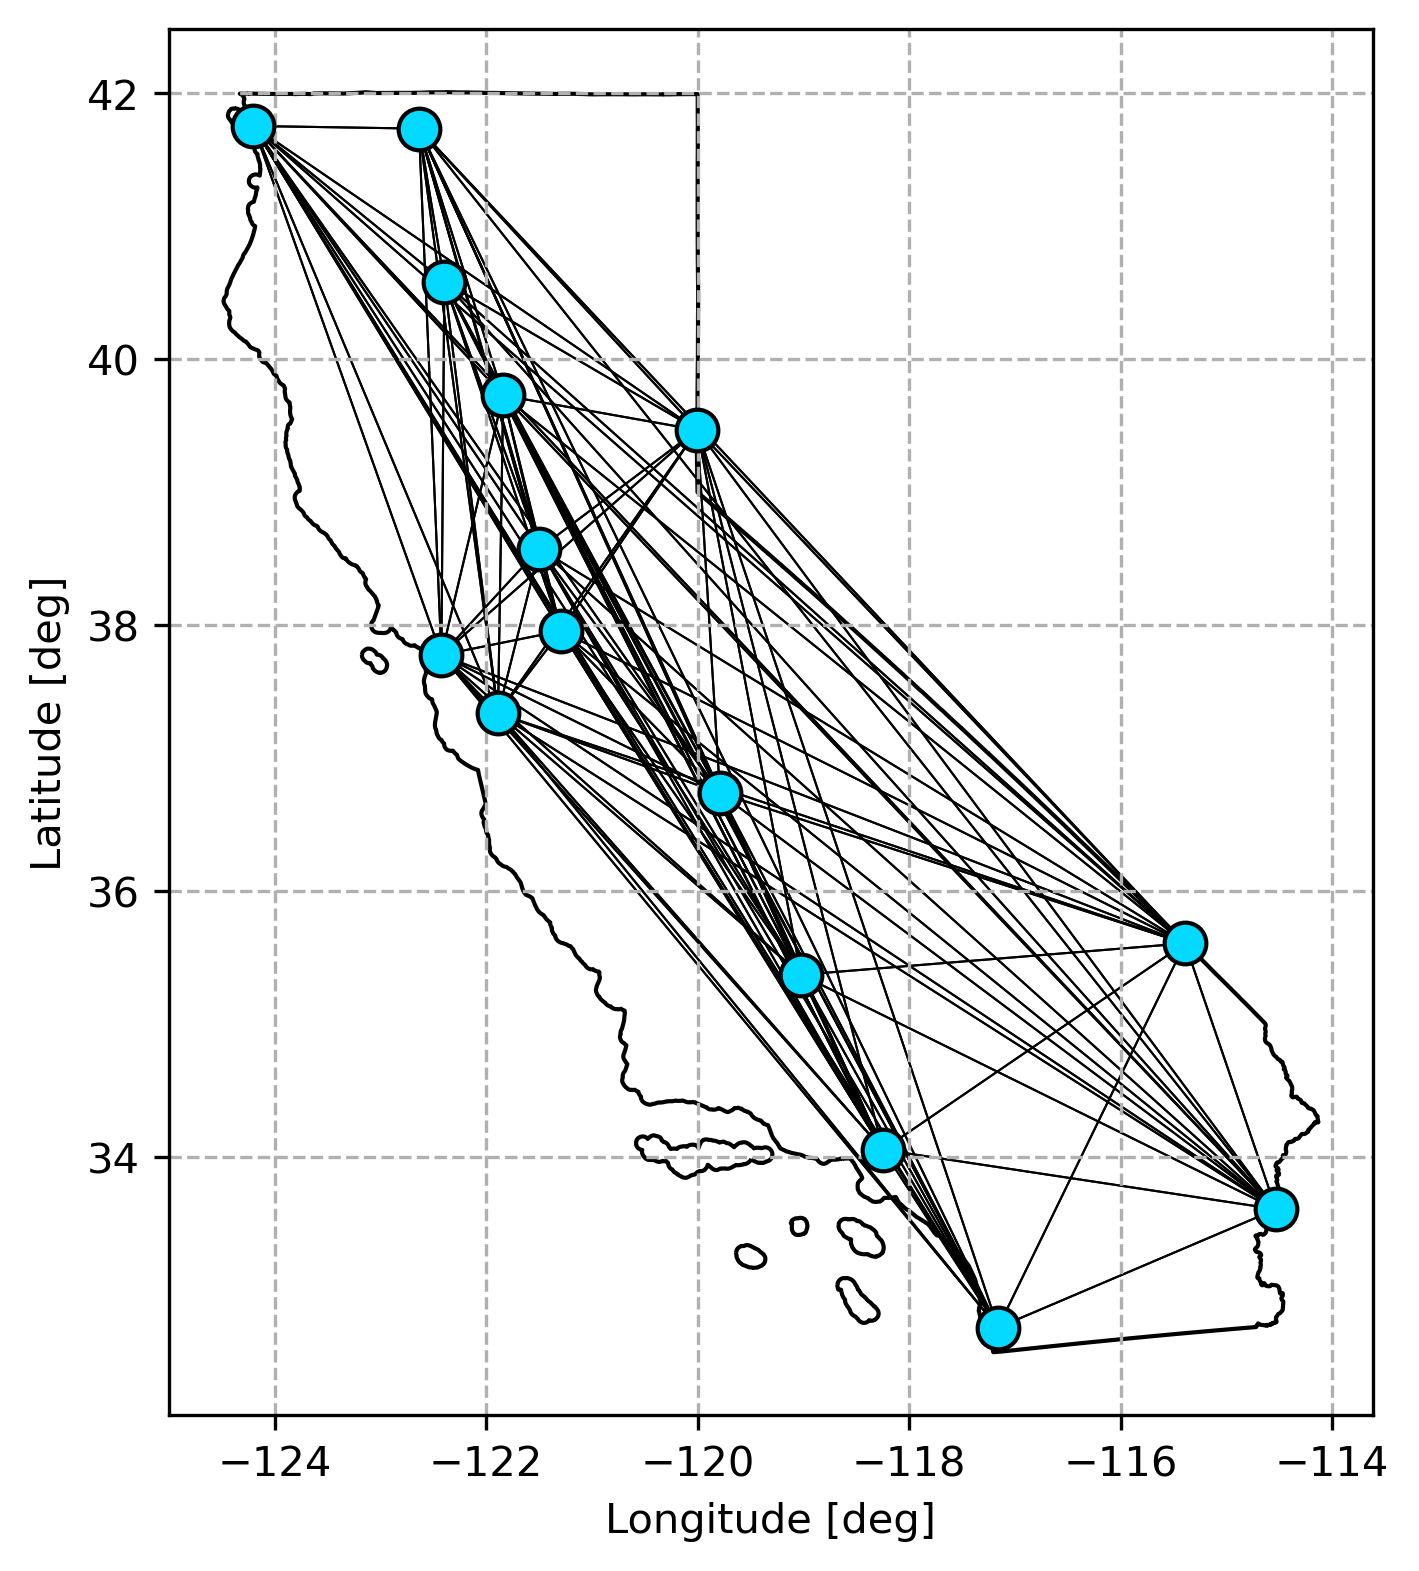
\includegraphics[width = \linewidth]{figs/reduced_graph.png}
	\end{subfigure}
	\caption{Example original graph (left) containing locations and an atlas and reduced subgraph (right) containing locations and arcs.}
	\label{fig:reduced_subgraph}
\end{figure}

Most of the nodes on the \gls{sng} will be supply stations each with different equipment types and numbers of ports. In-station redundancy for a \gls{sng} is a nodal parameter. In-station redundancy $\xi_{is}$ for any node $v \in V$ on \gls{sng} $G = \{V, E\}$ is the number of ports at node $v$. Between-station redundancy $\xi_{bs}$ for an \gls{sng} can be computed for cliques of nodes after solving the maximal clique problem. Between-station redundancy for any clique $C \subseteq V$ on \gls{sng} $G = \{V, E\}$ is the sum of the ports at nodes $v \in C$. Meaningful cliques may be attained by removing edges above a set cost before solving for maximal cliques. For example, cliques may be found on $G' = \{V, E'\}$ where $E' \subseteq E$ contains all edges of less than 10 minutes drive time.

The \gls{sng} is the graph on which long vehicle trips should be optimized if supply events are expensive and/or constraining. The relevant \gls{sng} for \glspl{icev} and \gls{bev} are neither equivalent nor isomorphic. Different vehicles within a given powertrain type may also have different \glspl{sng} but this is far more common for \glspl{ev} than \glspl{icev}. The \gls{sng} informs routing by providing a set of possible paths between origins and destinations. The structure of a network may make for a greater or lesser number of available paths depending on the number and location of stations.

\subsubsection*{Driver Model}

Different drivers will have different perceptions of cost for the same fundamentals based on their priorities and risk attitudes. In a basic sense, drivers will prioritize factors such as time, money, distance, and complexity differently. These priorities are modeled by computing overall cost as a linear combination of individual costs using constant weights. Route composite cost is computed as

\begin{equation}
	J(P_{i,j}) = \sum_{k = 0}^{M}\Phi_k(P_{i,j})
\end{equation}

where $P_{i,j}$ is a candidate route for arc $(i,j)$. The cost functions $\Phi$ will scale with the state values of $P_{i,j}$. In this study, all cost functions are linear multipliers. As such, the driver model is parameterized with the set of real-valued weights $\Omega$. Where any important factor is not known precisely drivers will consider a range of outcomes and decide based on an expectation. The result will be composite cost distribution $D$. Driver risk attitude concerns what range of outcomes will be used to compute expected cost. Risk attitude is modeled using a superquantile risk function defined as

\begin{equation}
	S(D, p_0, p_1) = \frac{1}{p_1 - p_0}\int_{p_0}^{p_1}Q(D, \alpha)\ d\alpha \label{eq:superquantile}
\end{equation}

\noindent where $p_0$ and $p_1$ are the boundaries of the range of probabilities considered in the expectation and $Q$ is the quantile function of $D$. The superquantile is, thus, the mean value of a distributed quantity within a range of probability. $S(D, 0, 1)$ reduces to the mean of $D$. Drivers with an aggressive risk attitude will consider a low range of probabilities. Drivers with a neutral attitude will consider a central range of probabilities. Drivers with a cautious attitude will consider a high range of probabilities. Driver parameters are listed in Table \ref{tab:param_driver}.

\begin{table}[H]
	\centering
	\caption{Supply Station Parameters for Routing}
	\label{tab:param_driver}
	\begin{tabular}{|C{\linewidth*3/8}|C{\linewidth*3/8}|C{\linewidth*2/8}|}
		\hline \rowcolor{lightgray} Parameter & Description & Unit \\
		\hline Priorities $\Omega$ & Set of multipliers for route costs to be used in computation of composite cost & [-] \\
		\hline Risk Attitude $(p_0, p_1)$ & Range of probabilities for superquantile function & [-] \\
		\hline
	\end{tabular}
\end{table}

The driver model serves to bias the routing by selecting a subset of information to use in optimization. As such it reflects individual perception. The results of the routing can be interpreted through the same bias, a different bias, or no bias. In this study, evaluation will be conducted on the basis of un-biased interpretation of costs.

\subsubsection*{Vehicle Model}

Vehicles effect routing due to their range limits and supply methods. The vehicle model used herein is highly simplified due to the inexact nature of the problem. Vehicles are modeled as storing energy and consuming energy at a constant rate per unit distance driven. More exact information on road conditions, traffic conditions, and atmospheric conditions among others can be used to compute edge-specific efficiencies. Vehicular parameters are listed in Table \ref{tab:param_veh}.

\begin{table}[H]
	\centering
	\caption{Vehicle Parameters for Routing}
	\label{tab:param_veh}
	\begin{tabular}{|C{\linewidth*3/8}|C{\linewidth*3/8}|C{\linewidth*2/8}|}
		\hline \rowcolor{lightgray} Parameter & Description & Unit \\
		\hline \gls{ess} Capacity & Accessible energy storage capacity & [kWh] \\
		\hline Energy Consumption & Energy required to move the vehicle & [kJ/km] \\
		\hline Maximum Supply Rate & \gls{ess} maximum energy addition rate & [kW] \\
		\hline Linear Charging Fraction & Percentage of the battery capacity which can be charged in the linear (constant current) range & [kW] \\
		\hline \gls{soc} Bounds & Range in which \gls{soc} must be maintained & [-] \\
		\hline
	\end{tabular}
\end{table}

DC charging is modeled using a CC-CV relationship wherein the first part of charging is linear and the second part follows exponential decay \cite{Marra_2012}. The inflection point which separates the linear and exponential decay sections is the Linear Charging Fraction $\eta$. The time required for a given charge event is

\begin{gather}
	\Delta T = \Delta T_{l} + \Delta T_{e} \\
	\Delta T_{l} = \begin{cases}
		\frac{(SOC_f - SOC_i) C}{\nu} &  SOC_i \leq SOC_f \leq \eta \\
		\frac{(\eta - SOC_i) C}{\nu} &  SOC_i \leq \eta \leq SOC_f \\
		0 &  \eta \leq SOC_i \leq SOC_f
	\end{cases} \\
	\Delta T_{e} = \begin{cases}
		0 & SOC_i \leq SOC_f \leq \eta \\
		-\frac{1}{\alpha}\ln{\left(1-\frac{SOC_f - \eta}{1-\eta}\right)} &  SOC_i \leq \eta \leq SOC_f \\
		-\frac{1}{\alpha}\ln{\left(1-\frac{SOC_f - SOC_i}{1-\eta}\right)} &  \eta \leq SOC_i \leq SOC_f \\
	\end{cases} \\
	\alpha = \frac{\nu}{\eta C}
\end{gather}

Where $C$ is the vehicle \gls{ess} capacity, $\nu$ is the actual power of the charge event, $\Delta T_l$ and $\Delta T_e$ are the time spent in the linear and exponential decay portions of the charge event, and $SOC_i$ and $SOC_f$ are the initial and final values of \gls{soc} for the charge event. Charge events are modeled to occur at the minimum of the maximum powers for the vehicle and charger. A typical value for $\eta$ will be in the range of 0.7 to 0.8. DC charging for a given quantity of energy past $\eta$ will take substantially longer than the same quantity below $\eta$. The difference in effective charging rate may serve to favor more DC charge events in a given arc which terminate at a lower \gls{soc}.

\subsubsection*{Supply Station Model}

Supply station design parameters are number of ports, reliability of ports, and the maximum supply rate of ports. The probability of port availability at a station is determined by the rate at which vehicles arrive at the station and how long they spend at the station. In combination, these factors determine the likelihood of a port being usable and available as well as the likely duration of queue if no port is usable and available. Supply station parameters are listed in Table \ref{tab:param_supply}.

\begin{table}[H]
	\centering
	\caption{Supply Station Parameters}
	\label{tab:param_supply}
	\begin{tabular}{|C{\linewidth*2/8}|C{\linewidth*3/8}|C{\linewidth*3/8}|}
		\hline \rowcolor{lightgray} Parameter & Description & Unit \\
		\hline Supply Rate & Maximum rate of energy supply & [kW] \\
		\hline Ports & Number of chargers/pumps at a station which can be used simultaneously & [-] \\
		\hline Reliability & Percentage of the time that a given pump will be usable & [-] \\ 
		\hline
	\end{tabular}
\end{table}

Information on ports is taken from \gls{afdc} \cite{afdc_2023}, information on equipment reliability is taken from \cite{Rempel_2023}, and information on port supply rates is taken from Google Maps.

Queue waiting time is computed using the M/M/c queuing formula with parametric uncertainty. The expected waiting time in an M/M/c queue is computed as

\begin{gather}
	W_q = \pi_0\frac{\rho(c\rho)^c}{\lambda(1-\rho)^2c!}\\
	\pi_0=\left[\left(\sum_{k = 0}^{c - 1}\frac{(c\rho)^k}{k!}\right) + \frac{(c\rho)^c}{c!(1 - \rho)}\right]\\
	\rho = \frac{\lambda}{c\mu}
\end{gather}

where $\lambda$ is the arrival frequency, $\mu$ is the service completion frequency, $c$ is the number of homogeneous servers, $\rho$ is the ratio of arrival frequency to composite maximum service completion frequency, and $\pi_0$ is the probability of an empty system. M/M/c queues assume an exponential distribution for both arrival and service completion frequency centered on a known mean. Reflecting the lack of information on charger accessibility accessible to drivers, these parameters must be sampled from distributions. Arrival frequency is much more uncertain than service completion frequency for drivers unfamiliar with a station. As such the drivers are modeled as assuming that charge event times will reflect the time required to fulfill a charge event sampled from a normal distribution and then picking values of $\rho$ based on their risk attitudes. In this study, charging event times in minutes are sampled from the normal distribution $N(30, 10)$. The effects of $\rho$ and in-station redundancy are shown in Figure \ref{fig:reduncancy_rho_wq}.

\begin{figure}[H]
	\centering
	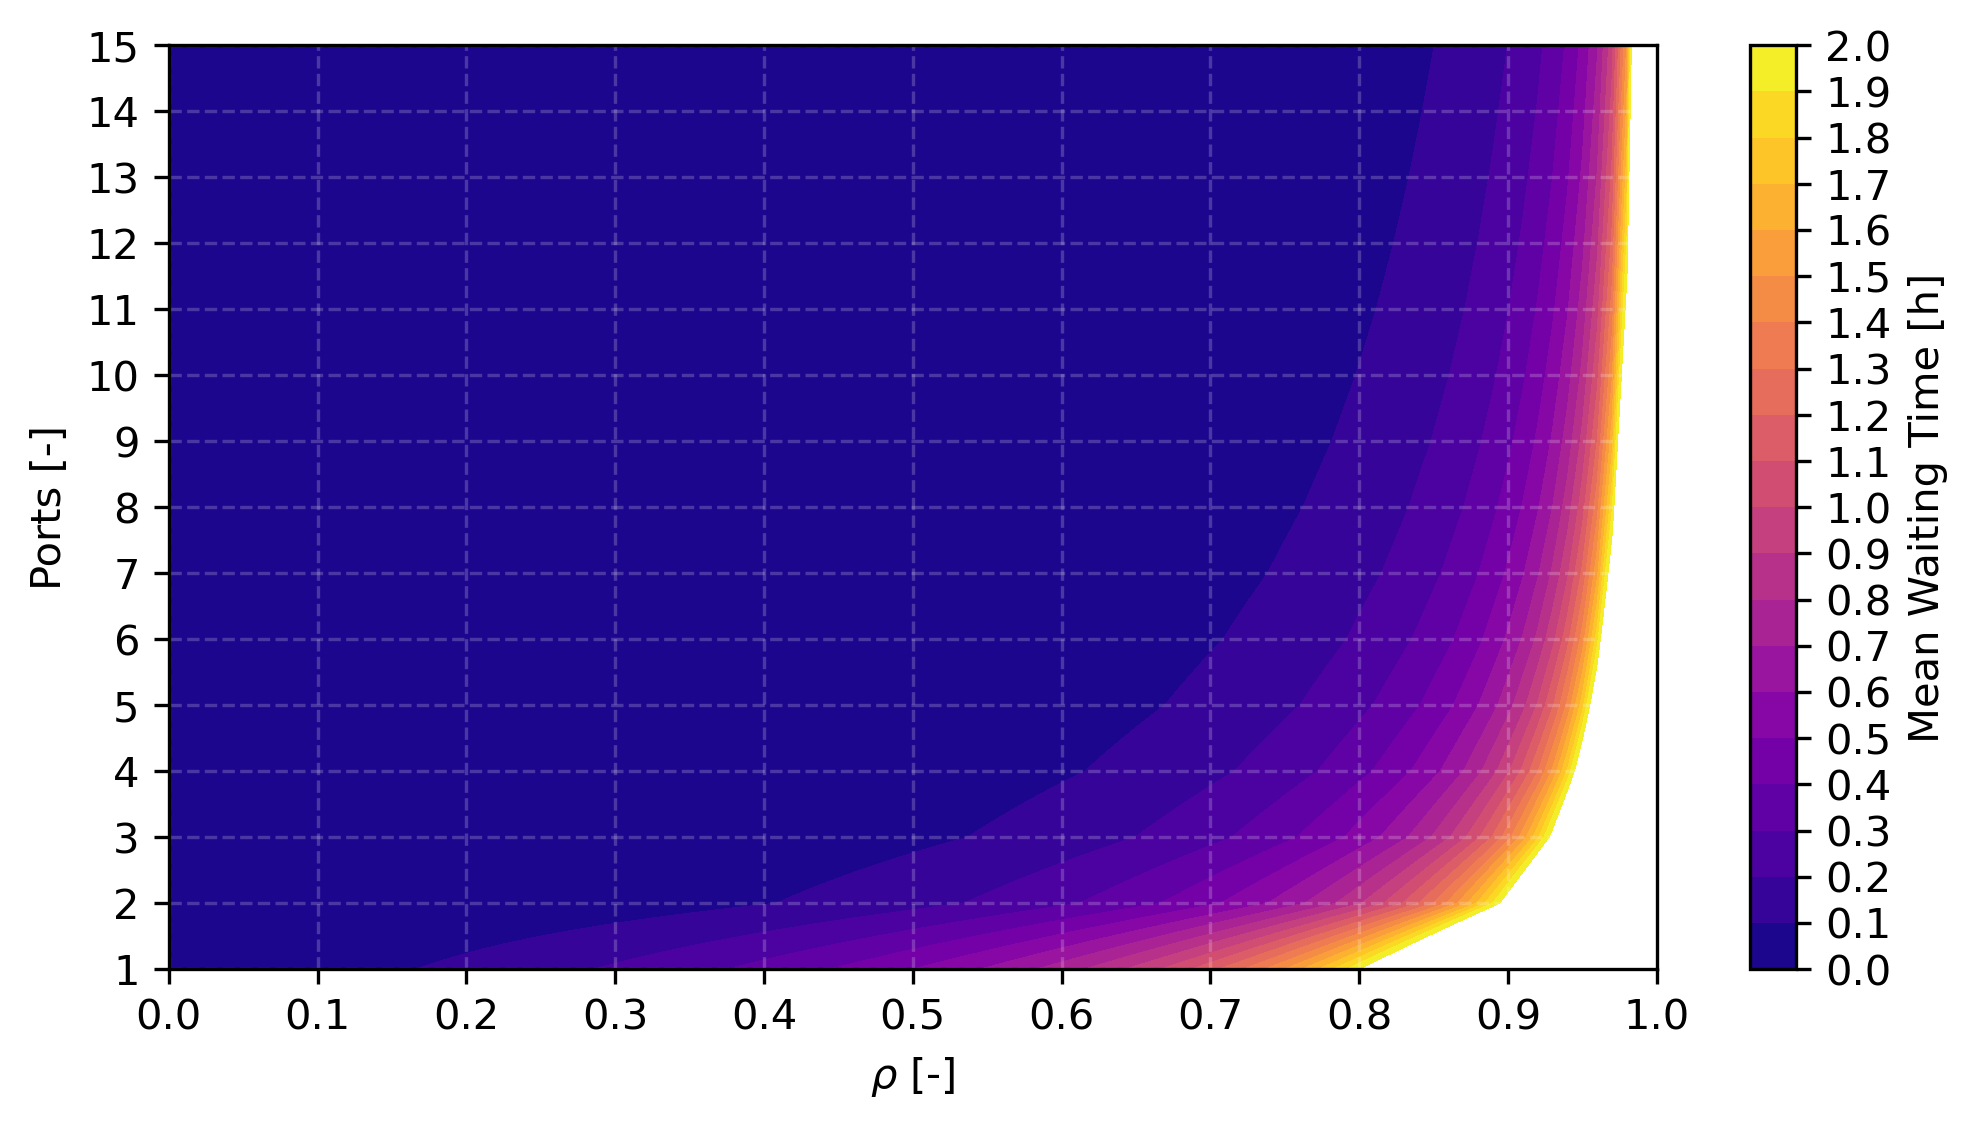
\includegraphics[width = \linewidth]{figs/waiting_time_rho_ports.png}
	\caption{Effects of in-station redundancy and $\rho$ on expected waiting time. Projected times of greater than 2 hours omitted in order to preserve scale.}
	\label{fig:reduncancy_rho_wq}
\end{figure}

Without prior information, a reasonable assumption is that a station will be sized, roughly, to meet demand. The $\rho$ parameter reflects the ratio of demand to maximum capacity and scales with redundancy all else being equal. However, unless completely saturated, a station with more port will be able to handle the same relative demand with a shorter queue due to heterogeneity in individual supply event times. With low demand, durable queues are unlikely to form at any station. As $\rho$ approaches 1, the expected duration of a queue grows toward infinity in a phenomenon known as queue instability. The rate of queue growth as a function of demand growth is determined by redundancy. In practice, a queue of sufficient length will be intolerable to any driver in almost any circumstance limiting queue growth. If this limit is 2 hours then, as seen in figure \ref{fig:reduncancy_rho_wq}, a cautious driver may view 1 and 2 port stations as ineligible.

\subsubsection*{Summary}

The Regional Impedance metric $Z_R$ quantifies the weighted average time of arcs between important locations in a region. $Z_R$ can be computed for any mode or set of modes. For the context of road vehicles, those vehicles which must resupply energy from different networks are, in effect, different modes. $Z_R$ is computed for a driver vehicle by building the relevant \gls{sng} and performing optimal routing based on the drivers preferences and perceptions and the physical characteristics of the vehicle and \gls{sng}. In this study the cost in question is total travel time. The total travel time is the combination of driving time, supply event time, and time spent queuing at supply stations. Each aspect of total travel time must be estimated by the driver with imperfect information when planning a route. Pure driving time is relatively knowable and a decent estimation may be obtained from many routing services. Supply event time is also relatively knowable, especially for experience drivers. Queue waiting time is far less knowable as accurate and timely information on charger utilization and equipment functionality is difficult to come by. Even where it is available beforehand, it may change by the time the driver arrives. These uncertainty and latency issues can substantially increase total travel times. In this study, queue waiting times are estimated by the driver based on the number of ports listed at a station while the actual queue waiting times are computed based on the number of functional ports. When equipment reliability is low drivers may end up spending more time than anticipated, especially if redundancy is also low. In the following case studies $Z_R$ is used as a metric of evaluation to study the impacts of model parameters on transportation accessibility.

%\section*{Randomly Generated Example}

The methods and metrics defined above are demonstrated using a vehicle on a randomly generated \gls{sng}. In this example, a \gls{sng} containing 15 locations and 85 stations distributed across a 1000 km square is generated with randomized node locations. Each location has a population of one million persons. Each station contains between 1 and 5 ports. Edges exist between all nodes and are assigned Pythagorean distances. All edges are assumed to be traversed at 105 kmh. The supply stations deliver an average of 45 kWh per vehicle at an average rate of 80 kW. The arrivals ratio is sampled from $N(1, 0.25)$ The vehicle used has a relatively low range of 262 km. Two drivers are modeled. A cautious driver is modeled using ($p_0 = 0.9$, $p_1 = 1.0$) and a aggressive driver is modeled using ($p_0 = 0$, $p_1 = 0.1$). Additionally port reliability at the stations is modeled as 75\% in a low reliability scenario and 95\% in a high reliability scenario.

\begin{figure}[H]
	\centering
	\begin{subfigure}[t]{.5\linewidth}
		\centering\captionsetup{width = .8\linewidth}
		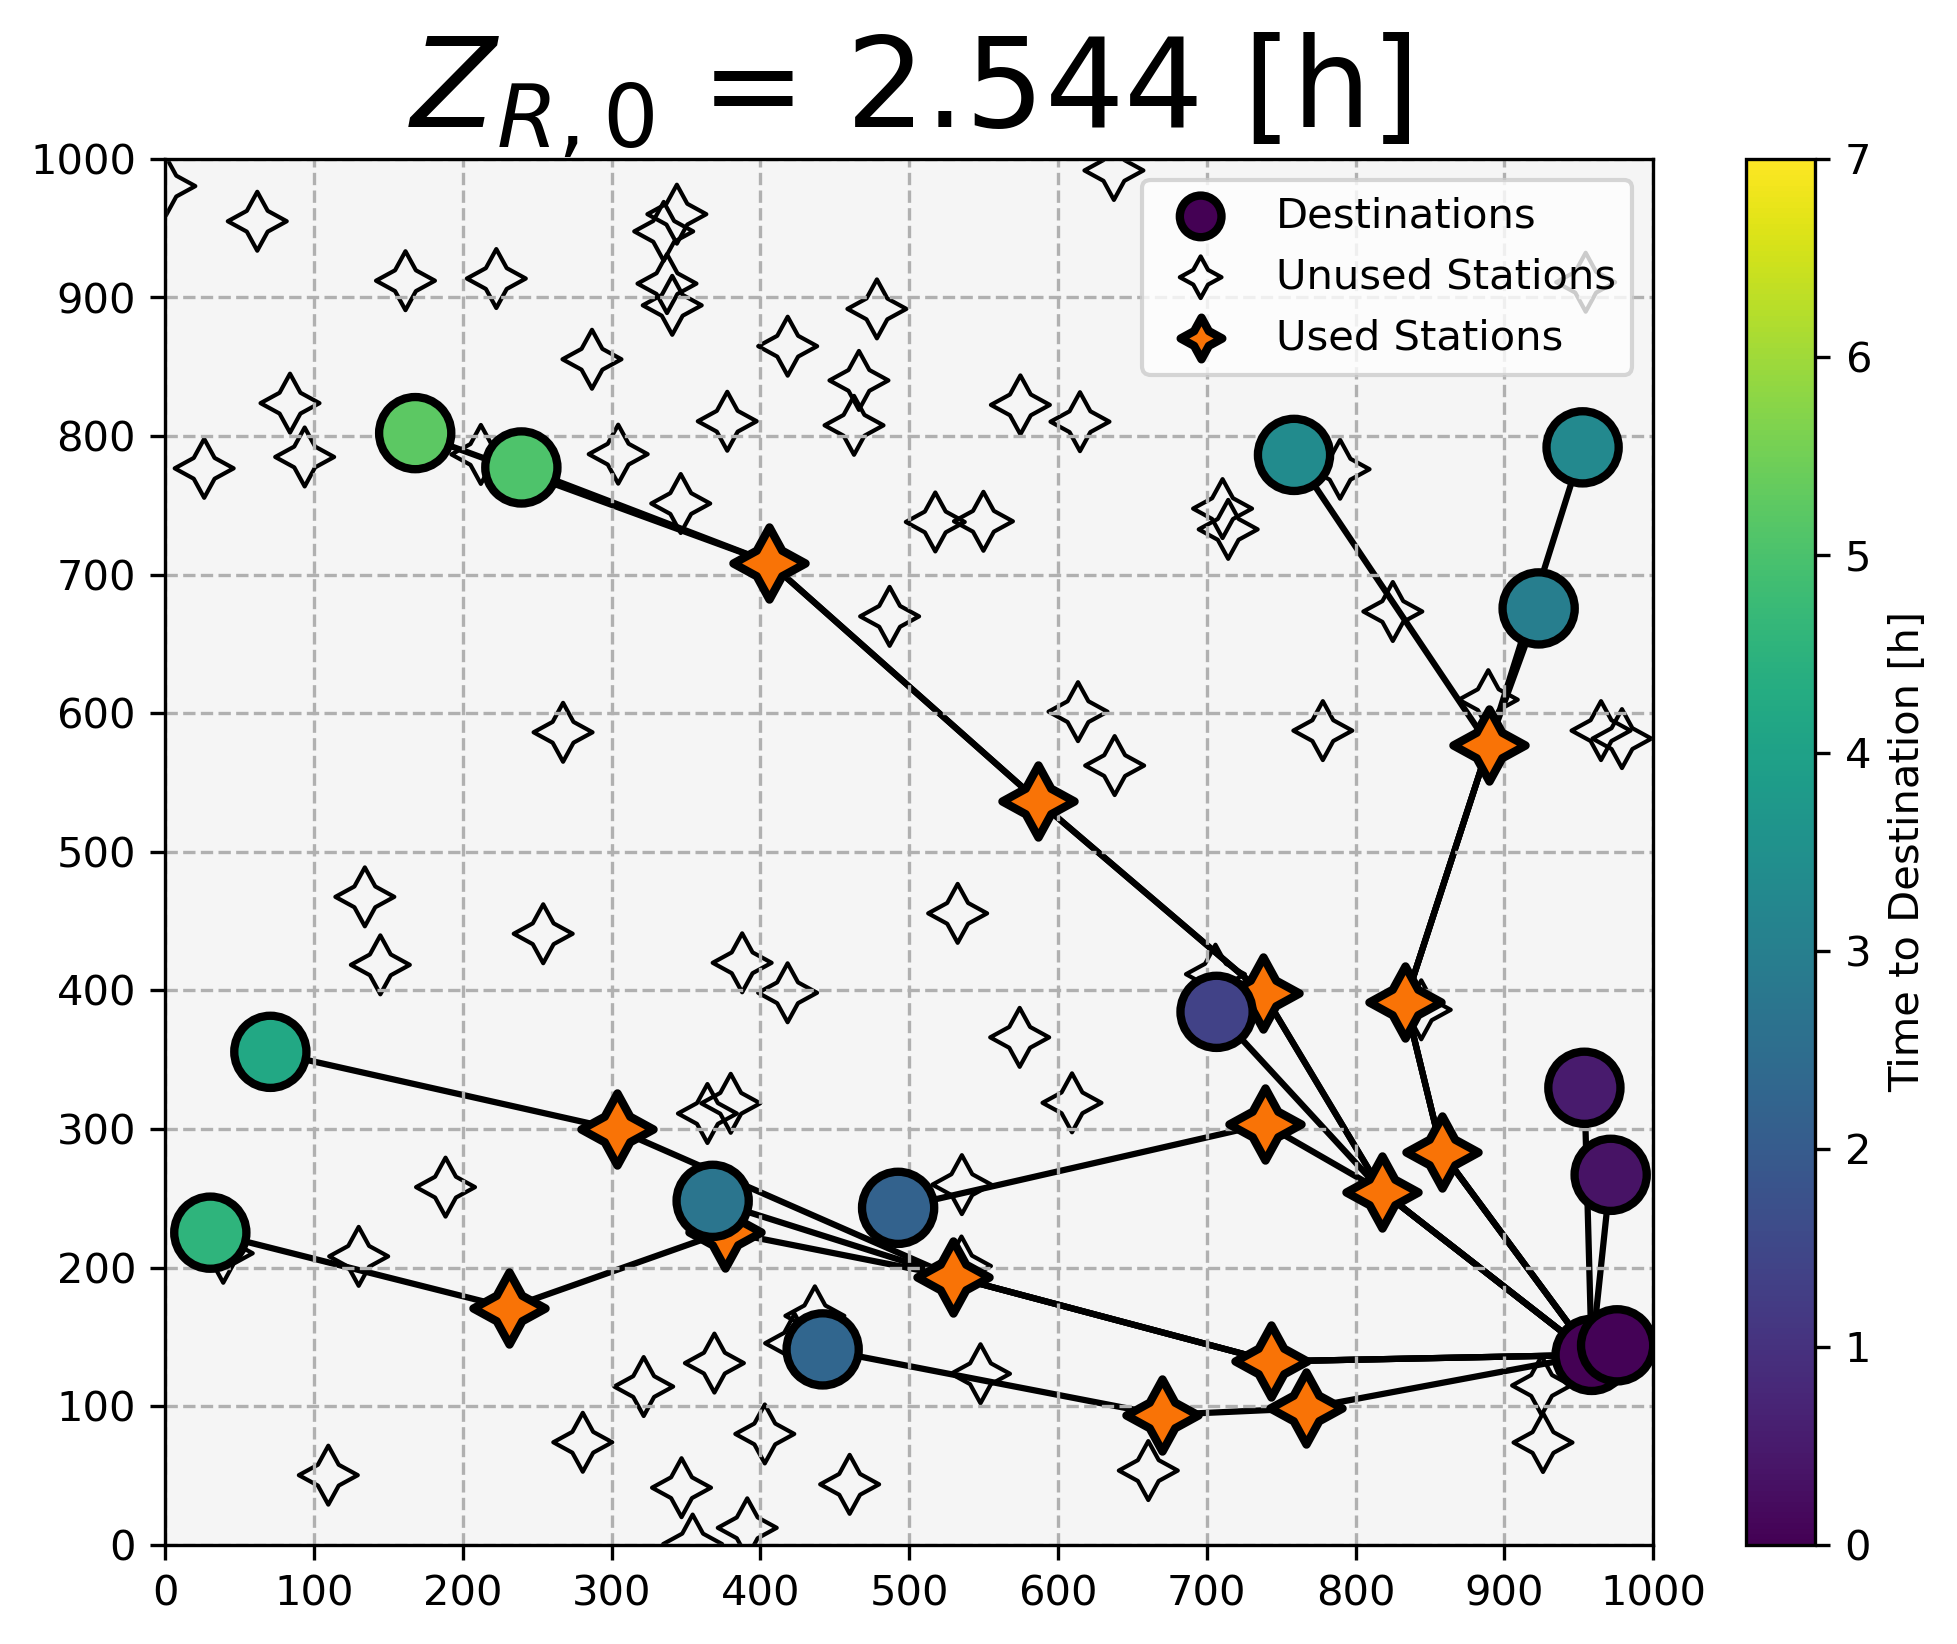
\includegraphics[width = \linewidth]{figs/random_example_high_reliability_aggressive_perceived.png}
		\caption{High reliability, aggressive}
	\end{subfigure}%
	\begin{subfigure}[t]{.5\linewidth}
		\centering\captionsetup{width = .8\linewidth}
		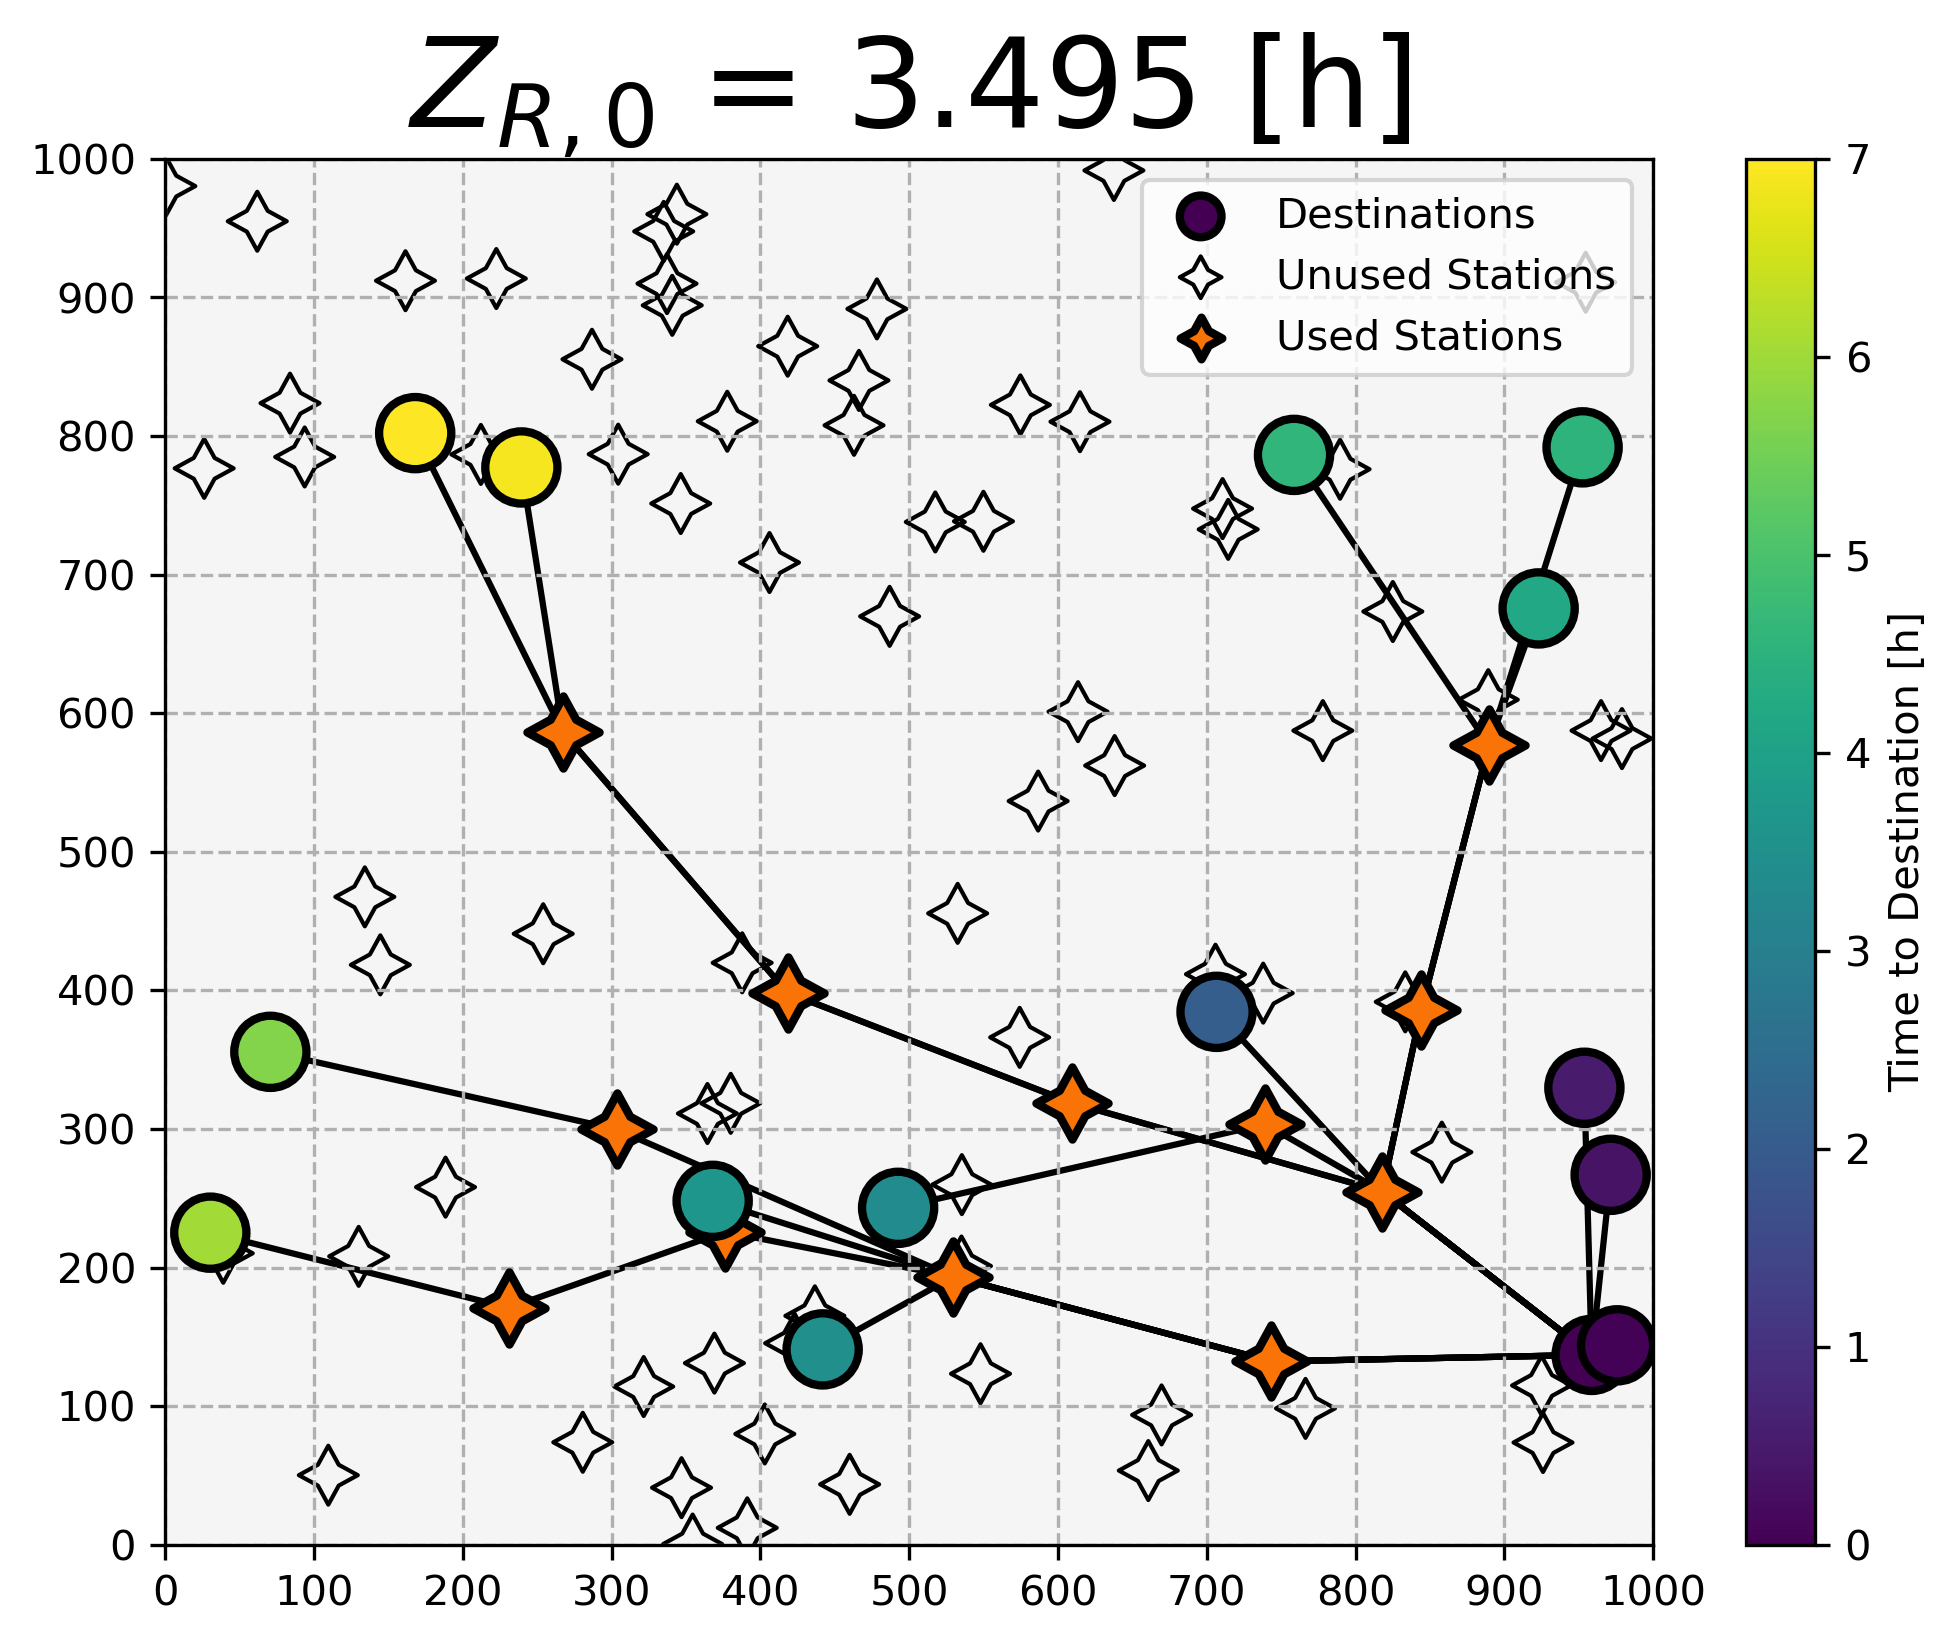
\includegraphics[width = \linewidth]{figs/random_example_high_reliability_cautious_perceived.png}
		\caption{High reliability, cautious}
	\end{subfigure}
	\begin{subfigure}[t]{.5\linewidth}
		\centering\captionsetup{width = .8\linewidth}
		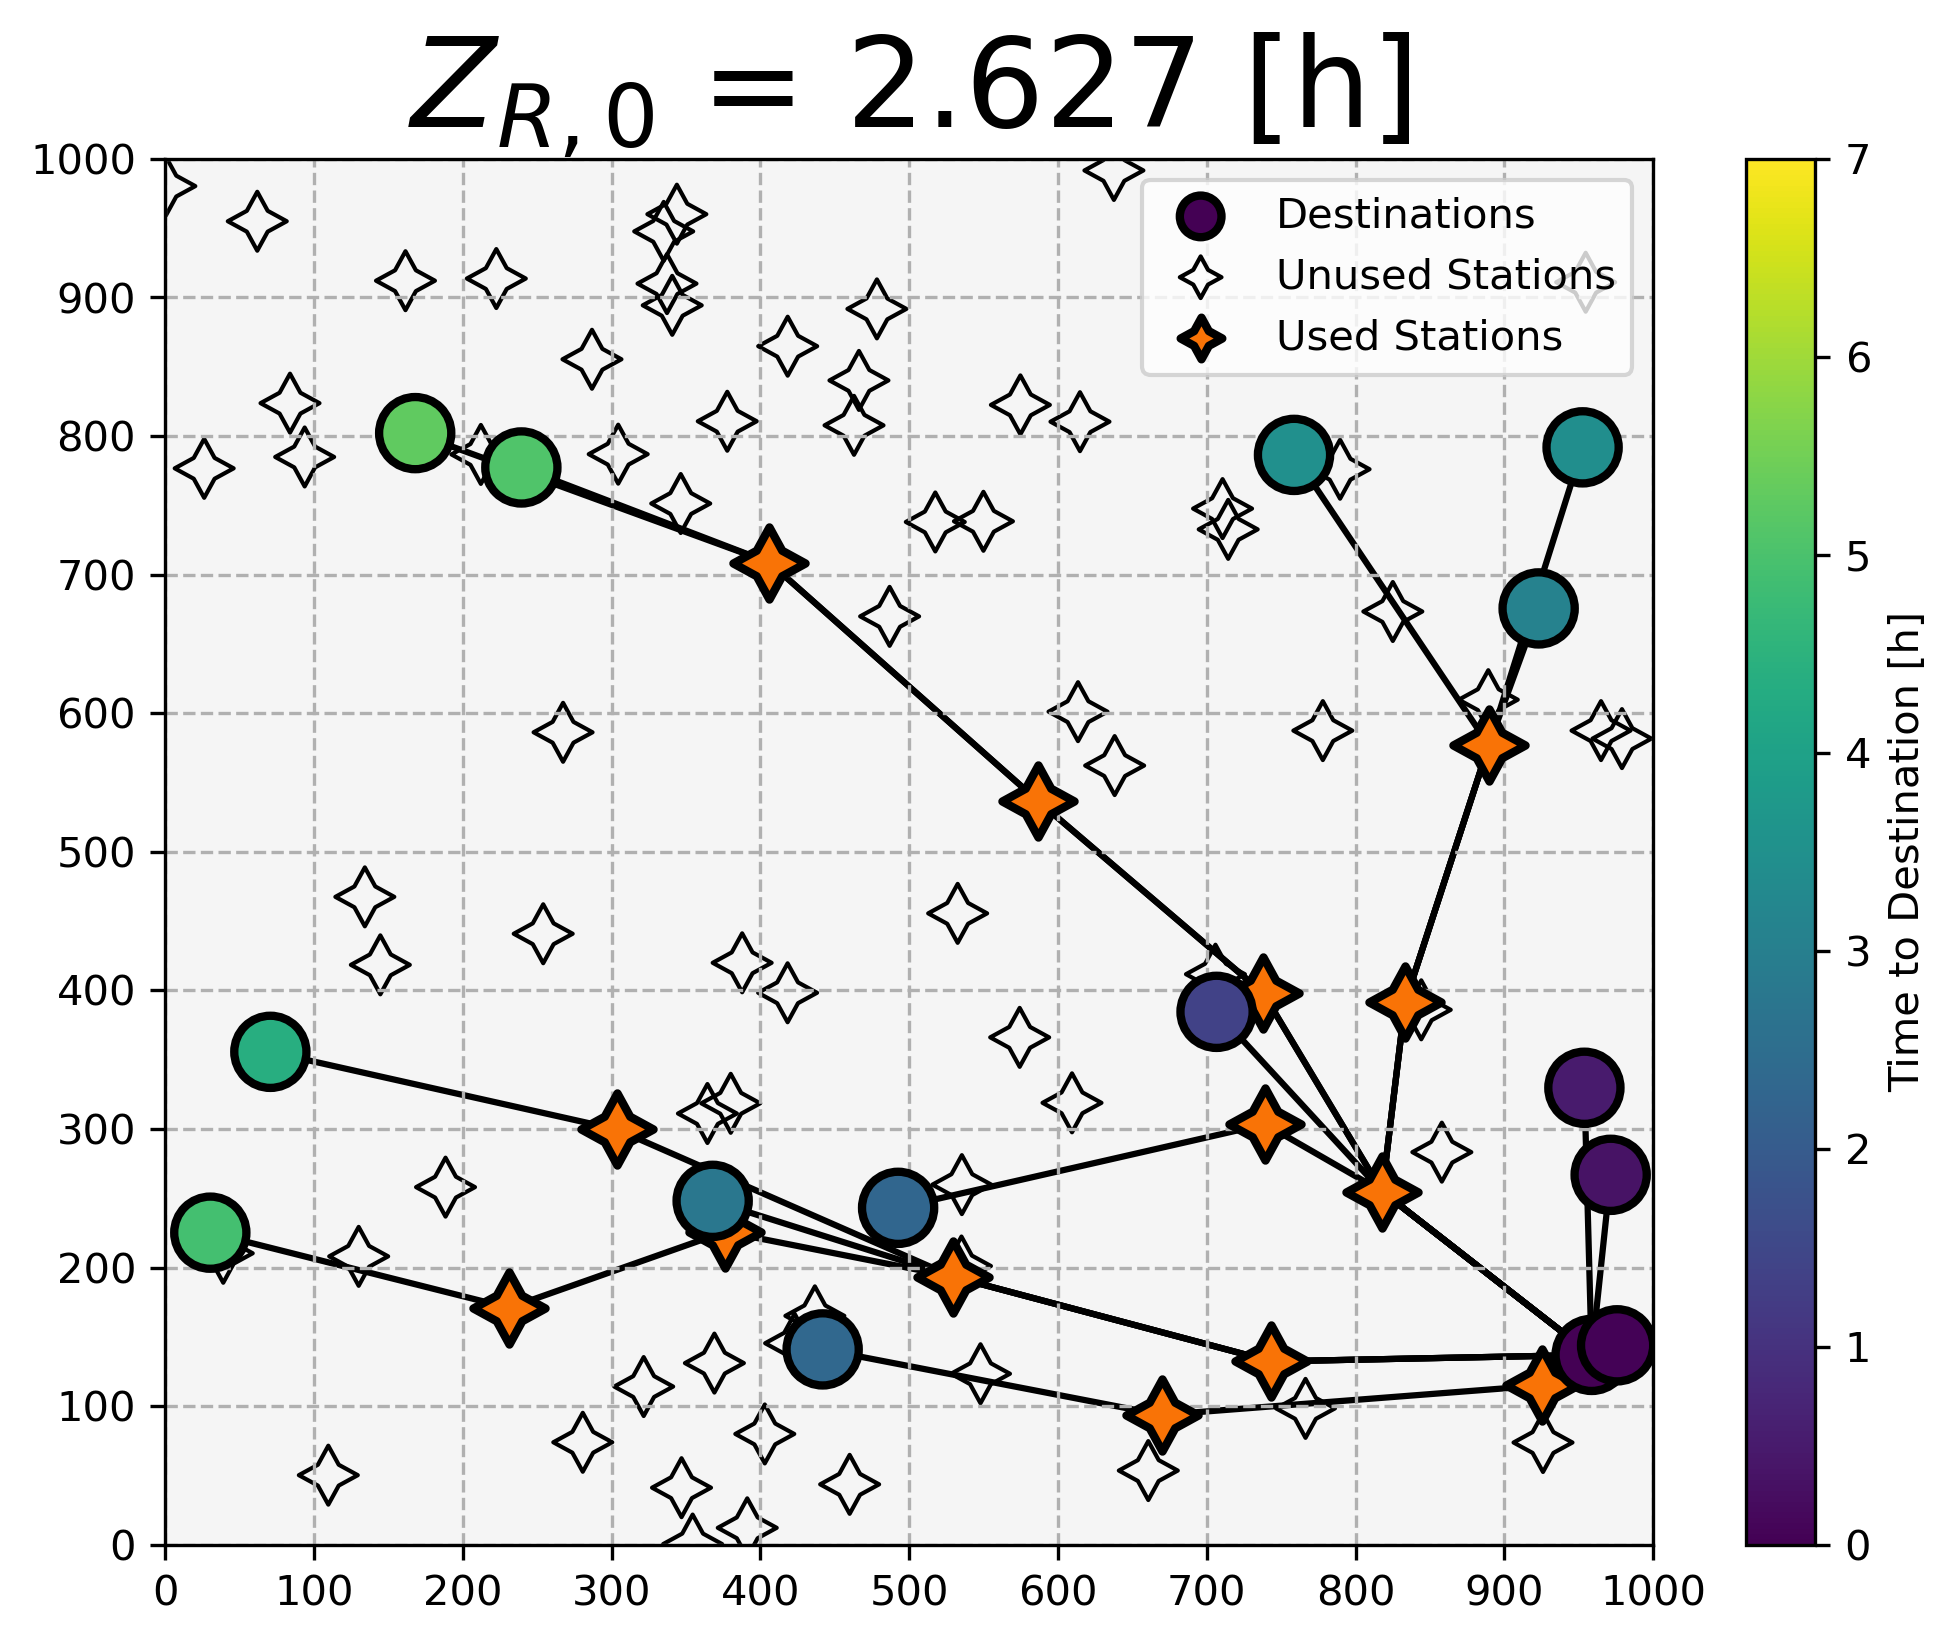
\includegraphics[width = \linewidth]{figs/random_example_low_reliability_aggressive_perceived.png}
		\caption{Low reliability, aggressive}
	\end{subfigure}%
	\begin{subfigure}[t]{.5\linewidth}
		\centering\captionsetup{width = .8\linewidth}
		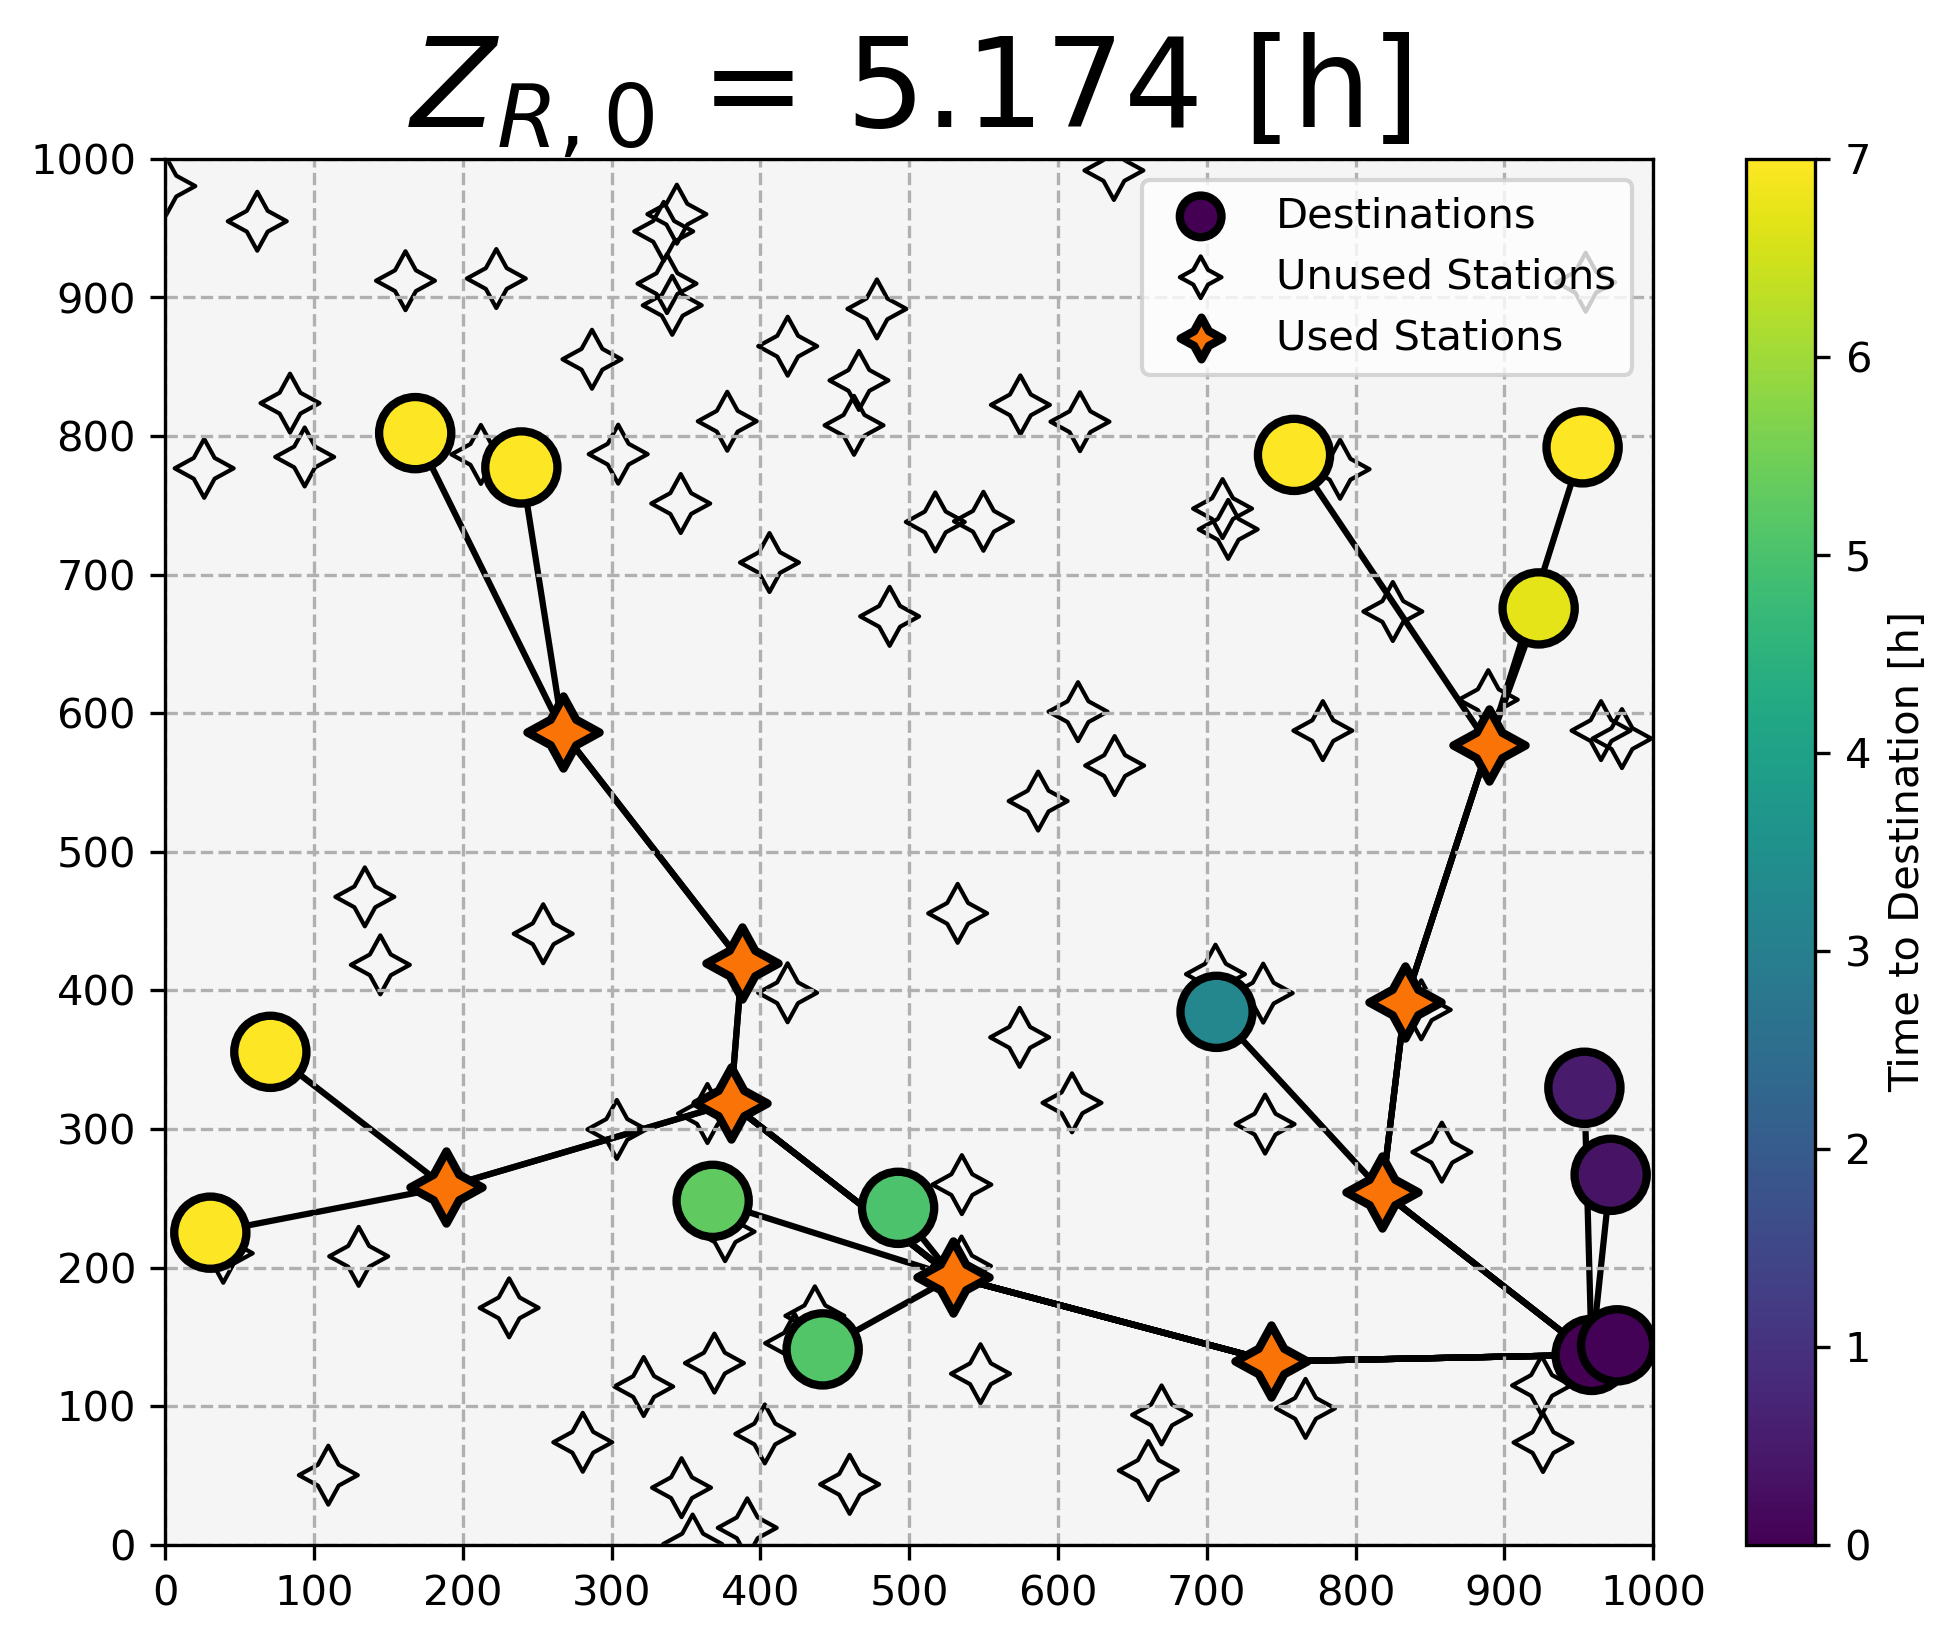
\includegraphics[width = \linewidth]{figs/random_example_low_reliability_cautious_perceived.png}
		\caption{Low reliability, cautious}
	\end{subfigure}
	\caption{Perceived Specific Regional Impedance by risk attitude and port reliability.}
	\label{fig:perceived_srta_random_perceived}
\end{figure}

The scenarios presented in Figure \ref{fig:perceived_srta_random_perceived} consider Specific Regional Impedance as perceived by the driver. The aggressive driver is only concerned with the best 10\% of outcomes where the cautious driver is only concerned with the worst 10\% of outcomes. The differences in perceived costs-to-travel are quite stark between the aggressive and cautious driver in both cases but this difference is larger when reliability is low. Drivers may operate off of perception but a regional transportation authority may be more concerned with mean outcomes. The neutral expectations ($p_0 = 0$, $p_1 = 1$) of the routes taken by the drivers are shown in Figure \ref{fig:perceived_srta_random_actual}.

\begin{figure}[H]
	\centering
	\begin{subfigure}[t]{.5\linewidth}
		\centering\captionsetup{width = .8\linewidth}
		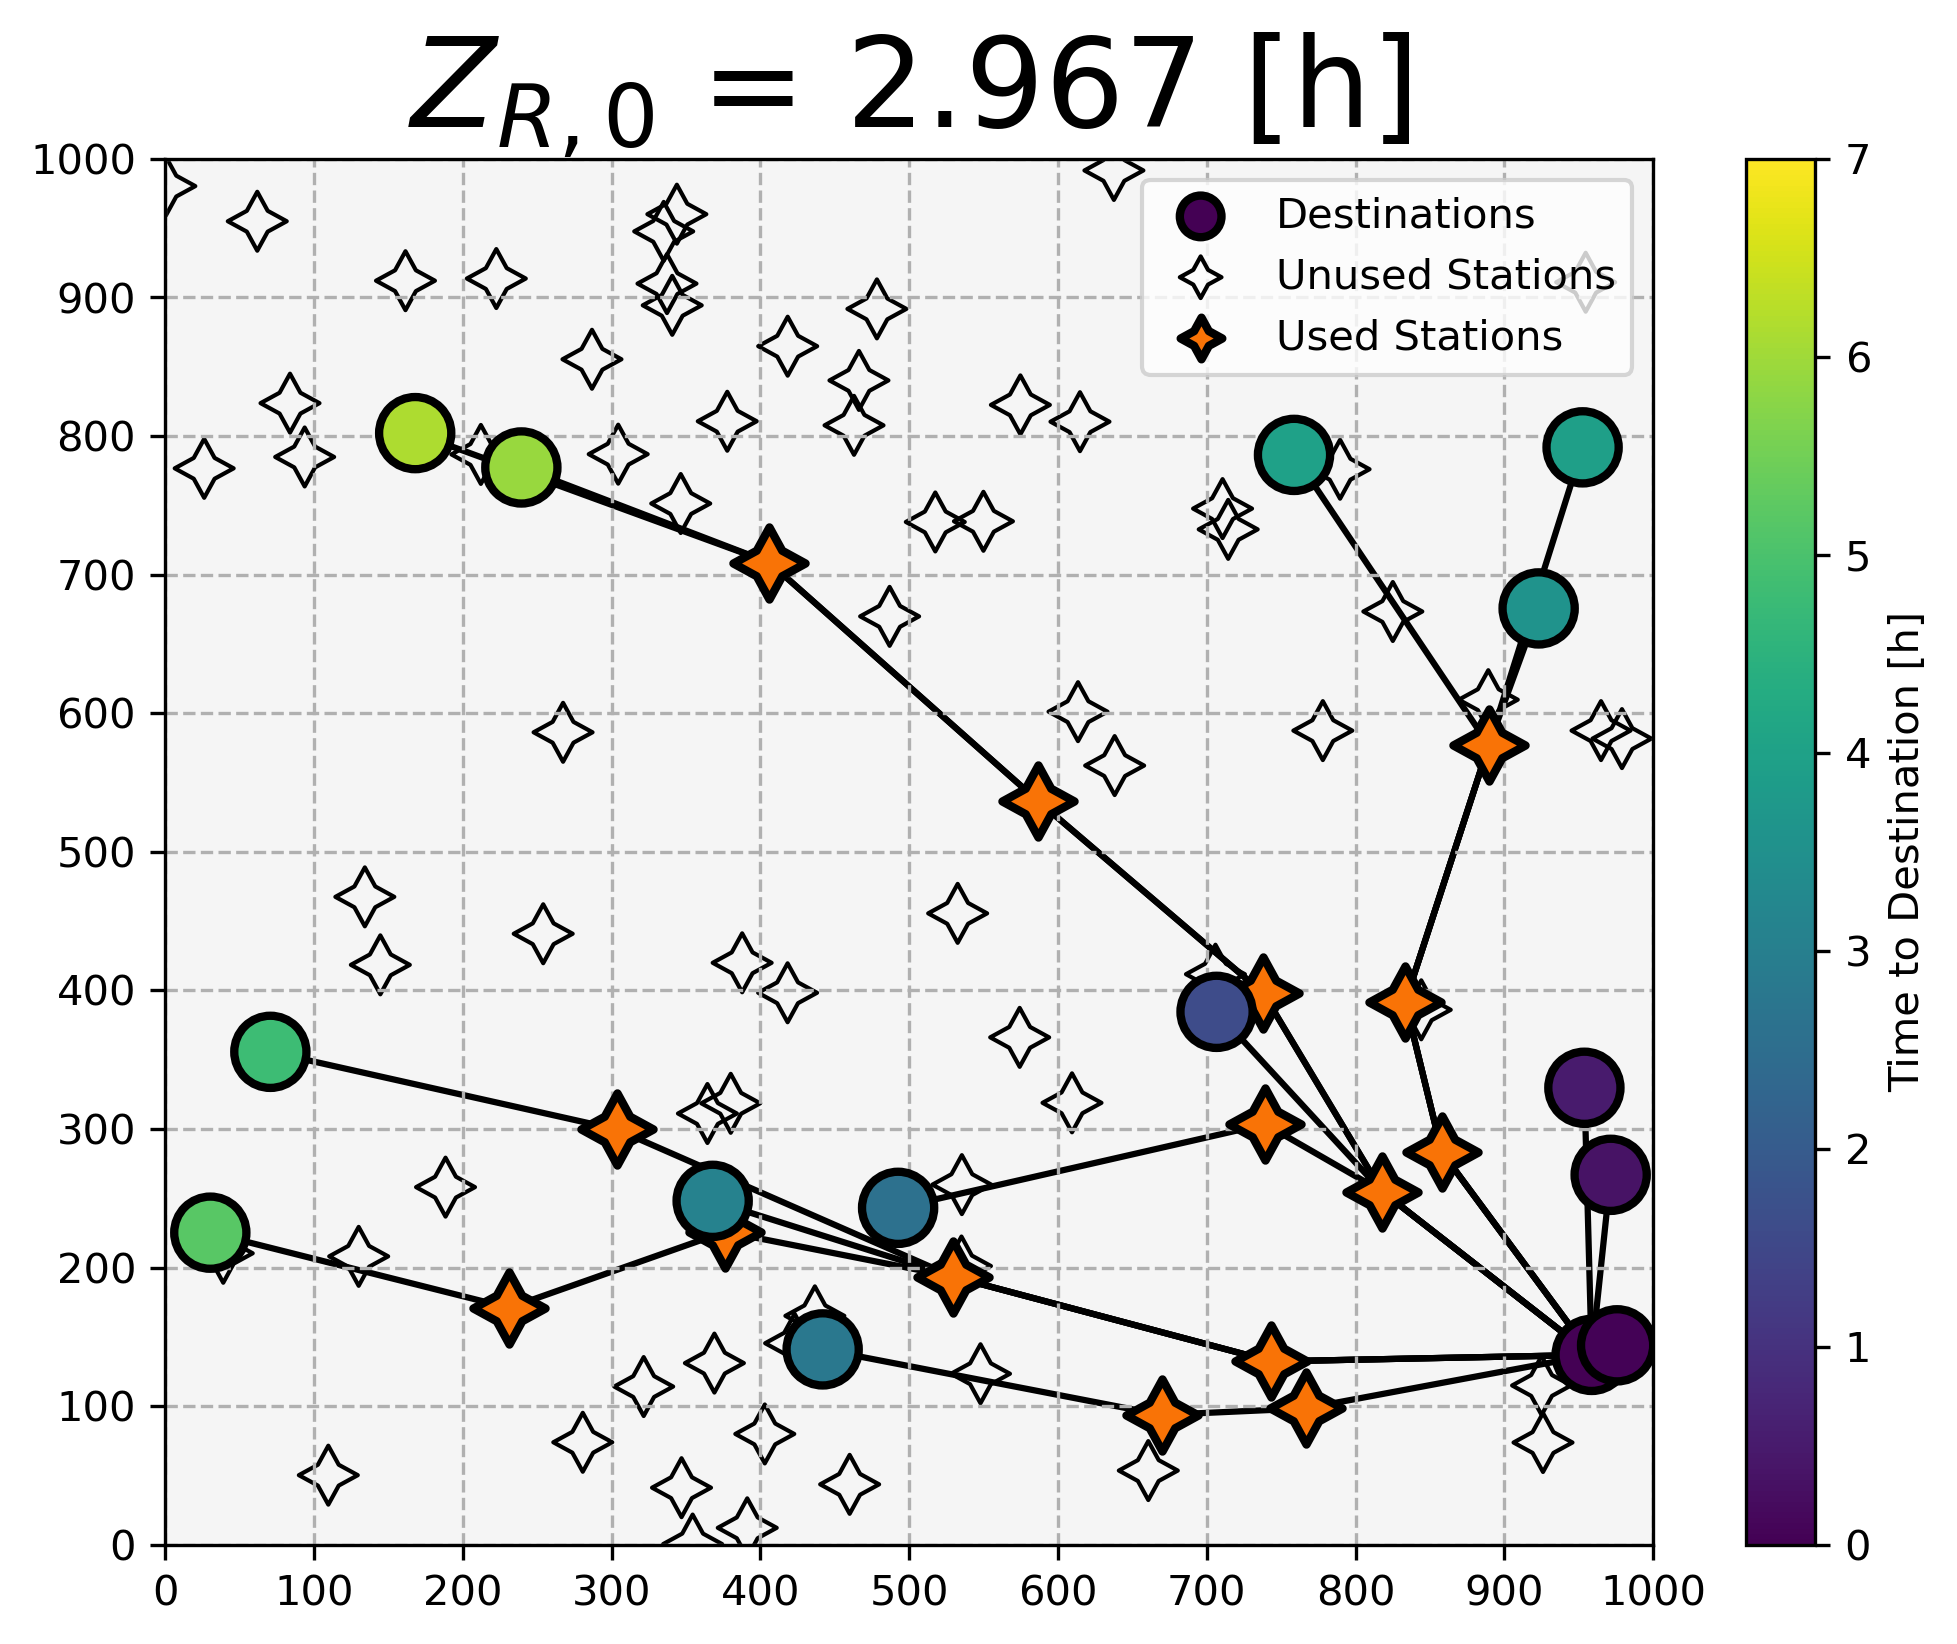
\includegraphics[width = \linewidth]{figs/random_example_high_reliability_aggressive_actual.png}
		\caption{High reliability, aggressive}
	\end{subfigure}%
	\begin{subfigure}[t]{.5\linewidth}
		\centering\captionsetup{width = .8\linewidth}
		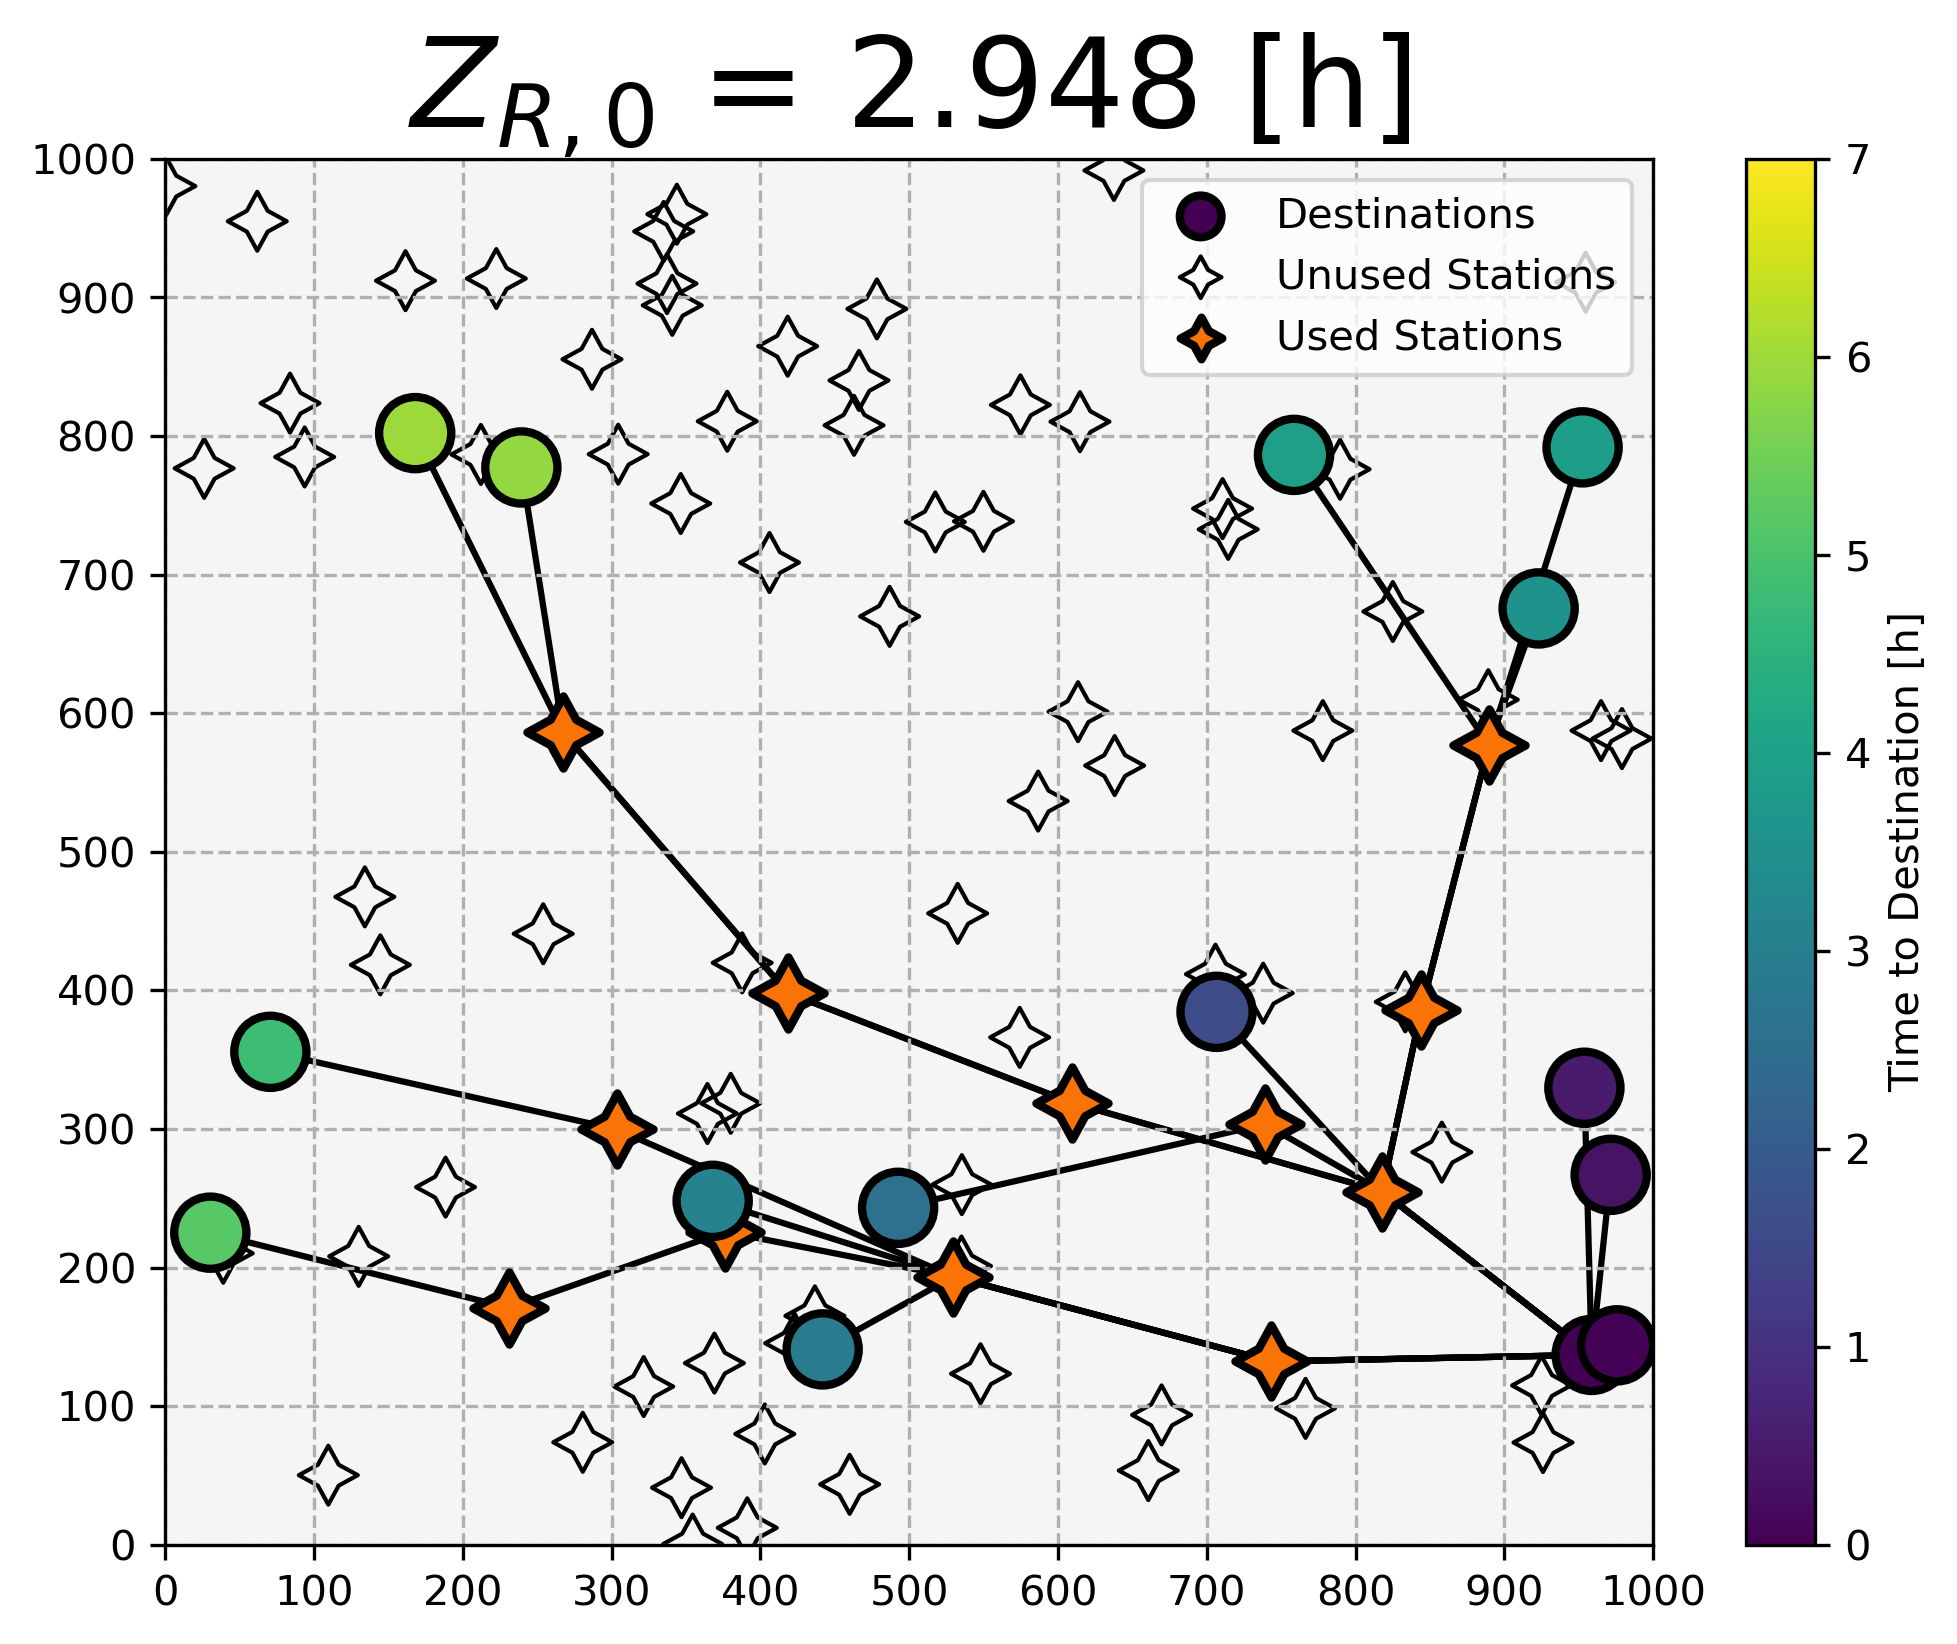
\includegraphics[width = \linewidth]{figs/random_example_high_reliability_cautious_actual.png}
		\caption{High reliability, cautious}
	\end{subfigure}
	\begin{subfigure}[t]{.5\linewidth}
		\centering\captionsetup{width = .8\linewidth}
		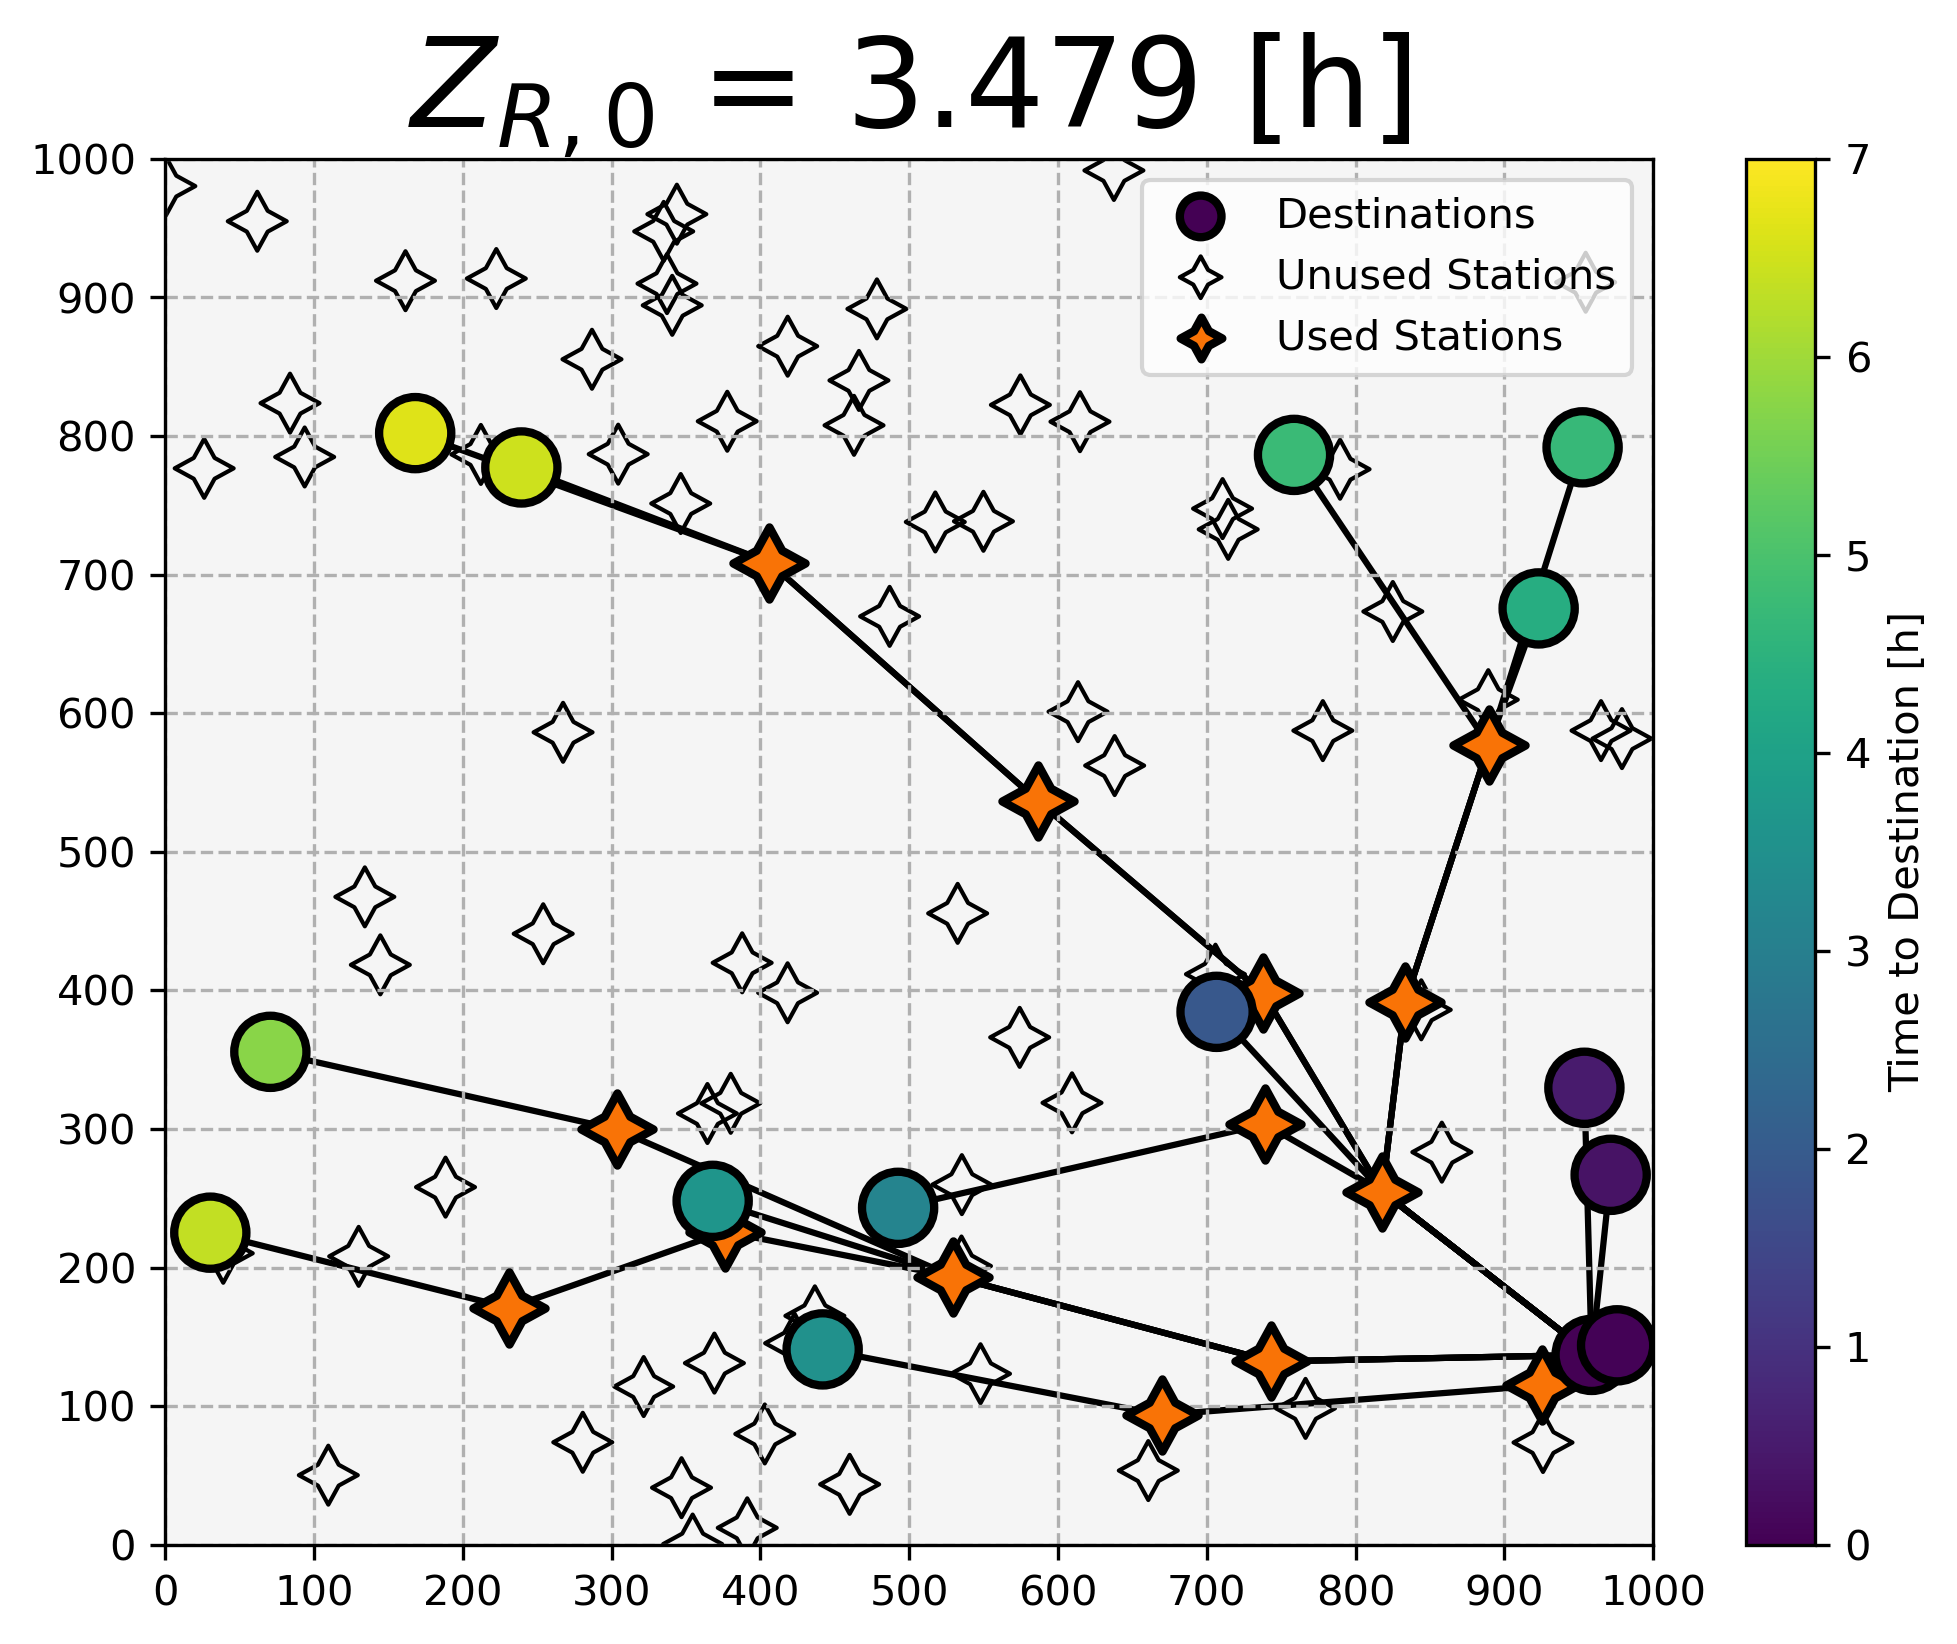
\includegraphics[width = \linewidth]{figs/random_example_low_reliability_aggressive_actual.png}
		\caption{Low reliability, aggressive}
	\end{subfigure}%
	\begin{subfigure}[t]{.5\linewidth}
		\centering\captionsetup{width = .8\linewidth}
		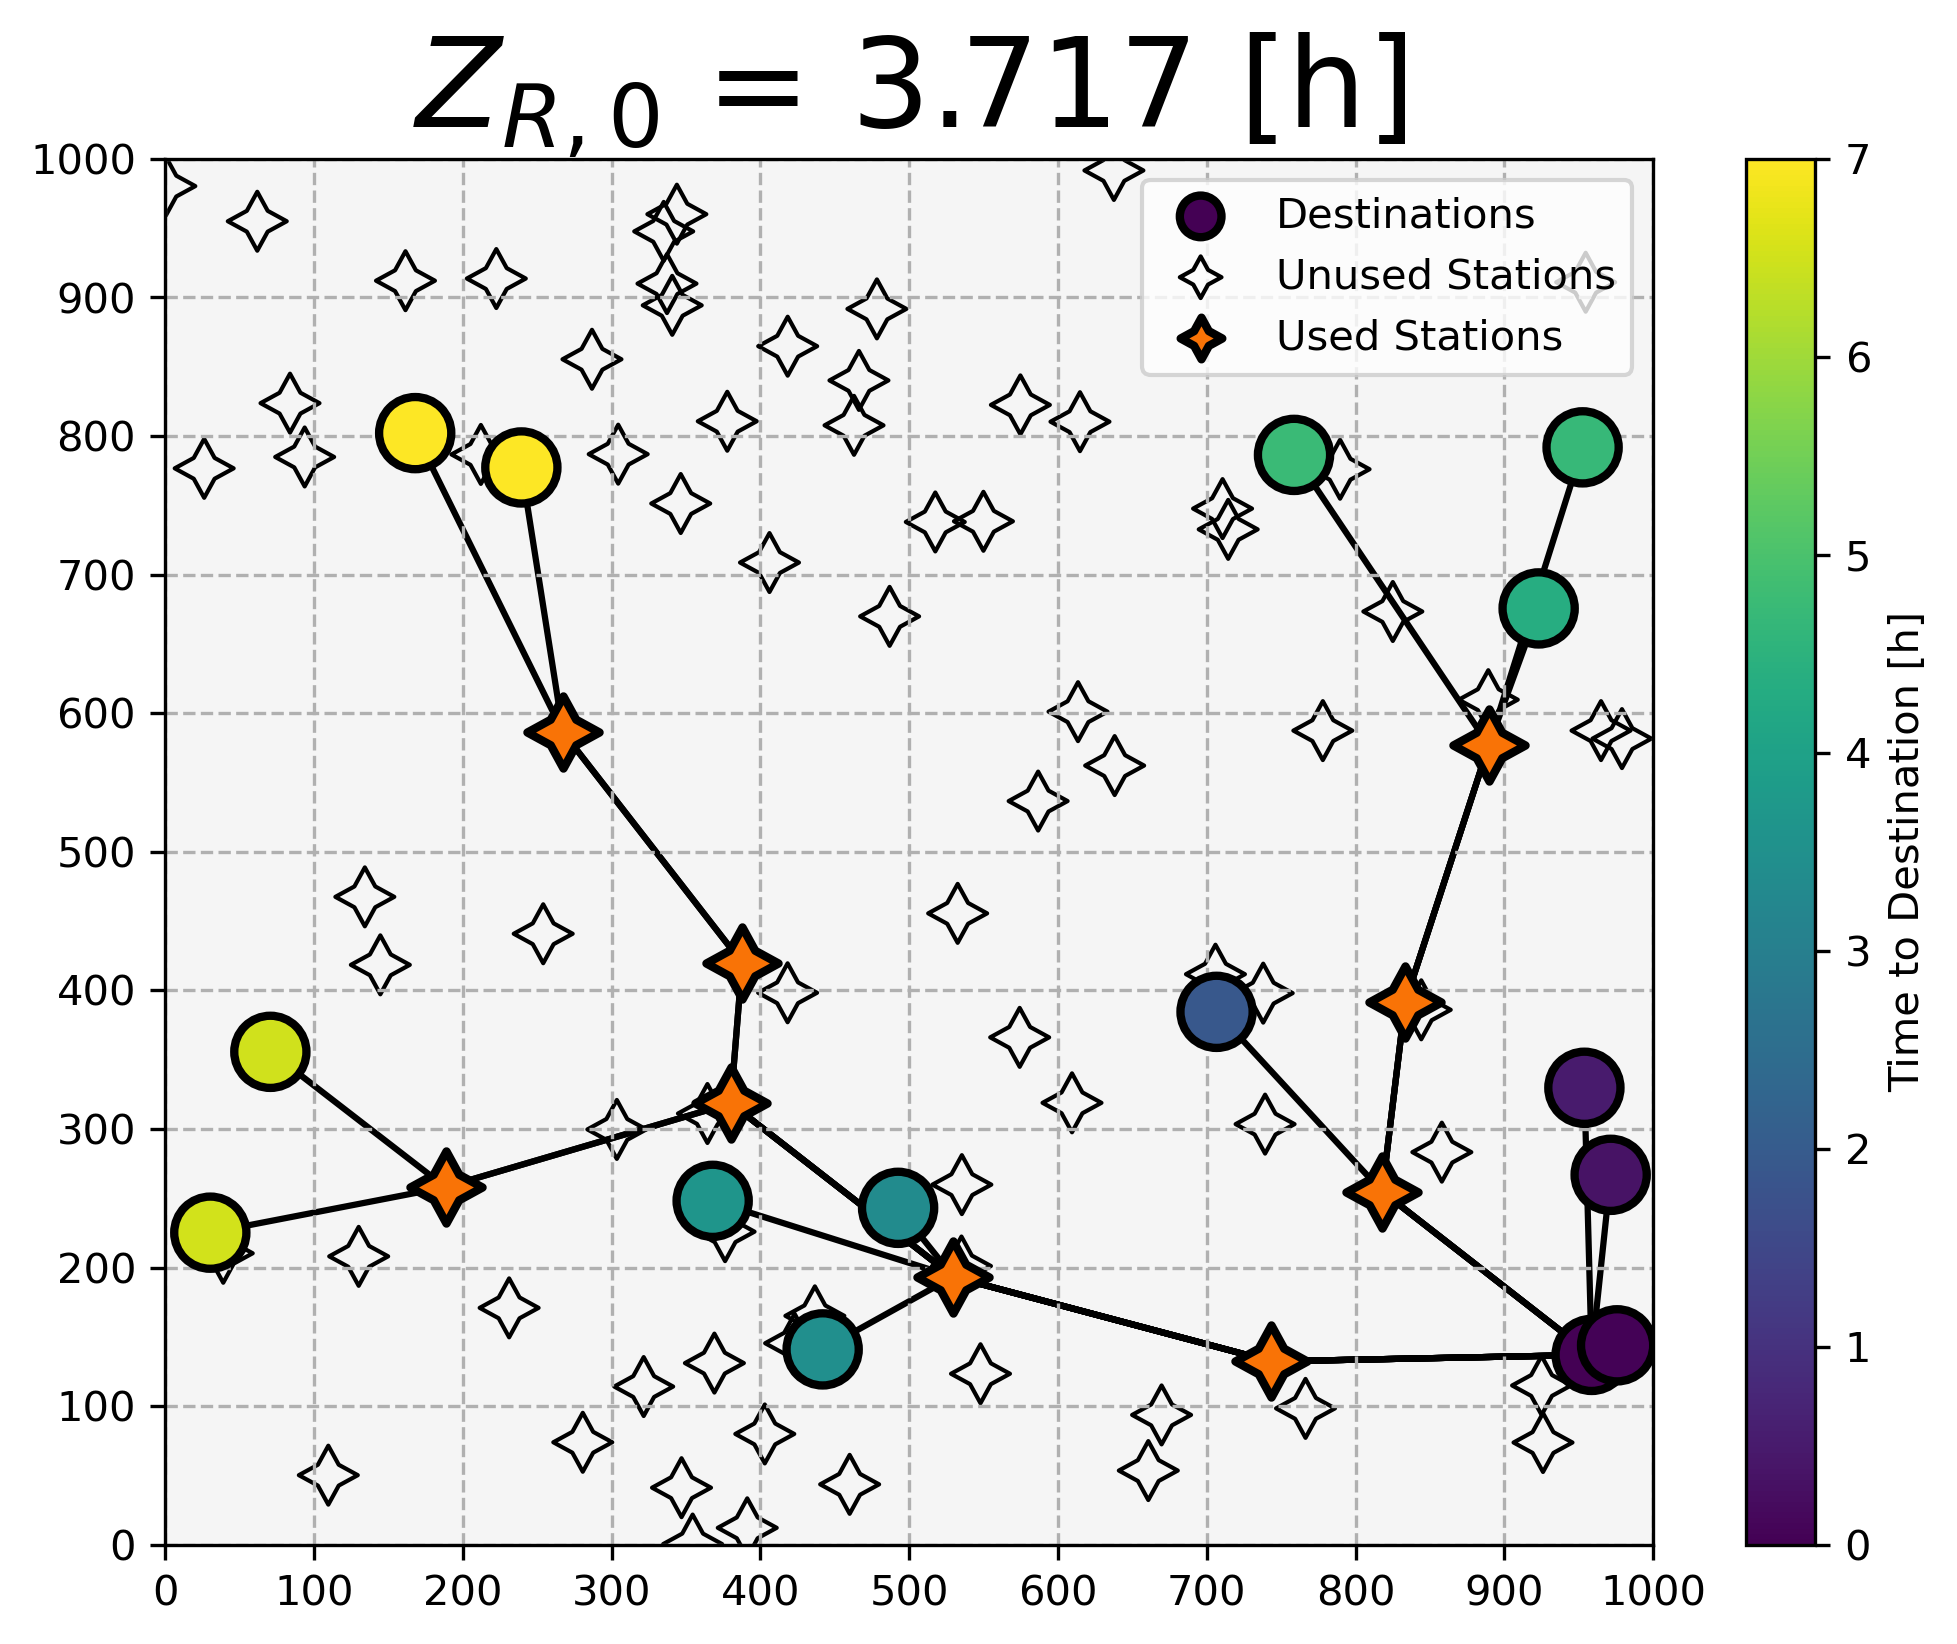
\includegraphics[width = \linewidth]{figs/random_example_low_reliability_cautious_actual.png}
		\caption{Low reliability, cautious}
	\end{subfigure}
	\caption{Neutral expectations of Specific Regional Impedance by risk attitude and port reliability.}
	\label{fig:perceived_srta_random_actual}
\end{figure}

The neutral expectations tell a different story. For the different levels of reliability, neutral expectations of impedance are similar for the routes selected by the aggressive and cautious drivers. The differences between biased and neutral perception are easy to understand. Both drivers selected routes based on a subset of the information and these routes are non-optimal when all information is considered. Drivers may adjust their priors over time but policy can only control the fundamentals. Thus, it is recommended to consider bias in route planning but neutral expectation in evaluation.

The composition of the routes taken by the drivers in the randomly generated example demonstrate an interesting dynamic as seen in Table \ref{tab:distances_redundancy}. As in-station redundancy is highly important in determining expected queuing times cautious drivers opt, increasingly for stations with higher in-station redundancy at the cost of taking less direct routes.

\begin{table}[H]
	\centering
	\caption{Average route distances and chargers per station utilized for example scenarios}
	\label{tab:distances_redundancy}
	\begin{tabular}{|C{\linewidth / 3}|C{\linewidth / 3}|C{\linewidth / 3}|}
		\hline Reliability & Risk-Attitude & Chargers per Station Utilized \\
		\hline High & Aggressive & 3.774 \\
		\hline High & Cautious & 4.258 \\
		\hline Low & Aggressive & 4.032 \\
		\hline Low & Cautious & 4.471 \\
		\hline
	\end{tabular}
\end{table}

\section*{California Case Study}

The randomly generated example is informative but does not reflect any actual \gls{sng}. In order to see effects on a more representative basis a case study is performed on the state of California using information on the states DC EV \gls{sng} with modes of common \glspl{bev} which enjoy different levels of access.

\subsection*{Background}

The state of California is geographically large and diverse in demography and land use. Per 2022 US census bureau annual estimates [SOURCE], California's population numbers over 39 million persons with around 32.5 million living in 482 Incorporated Places including cities and towns. These Places range from Los Angeles with a population of 3.8 million located near the coast to Amador City with a population of 201 located in the Sierra foothills. Connecting these disparate locations are a collection of major road transit corridors. Running roughly north-south are S-1/101, I-5/S-99, and U-395. Running roughly east-west are I-8, I-10, I-15, I-40, and I-80. Much of the traffic on the east-west corridors represents interactions with adjoining states. Incorporated Places in California are shown in Figure \ref{fig:california_incorporated_places}.

\begin{figure}[H]
	\centering
	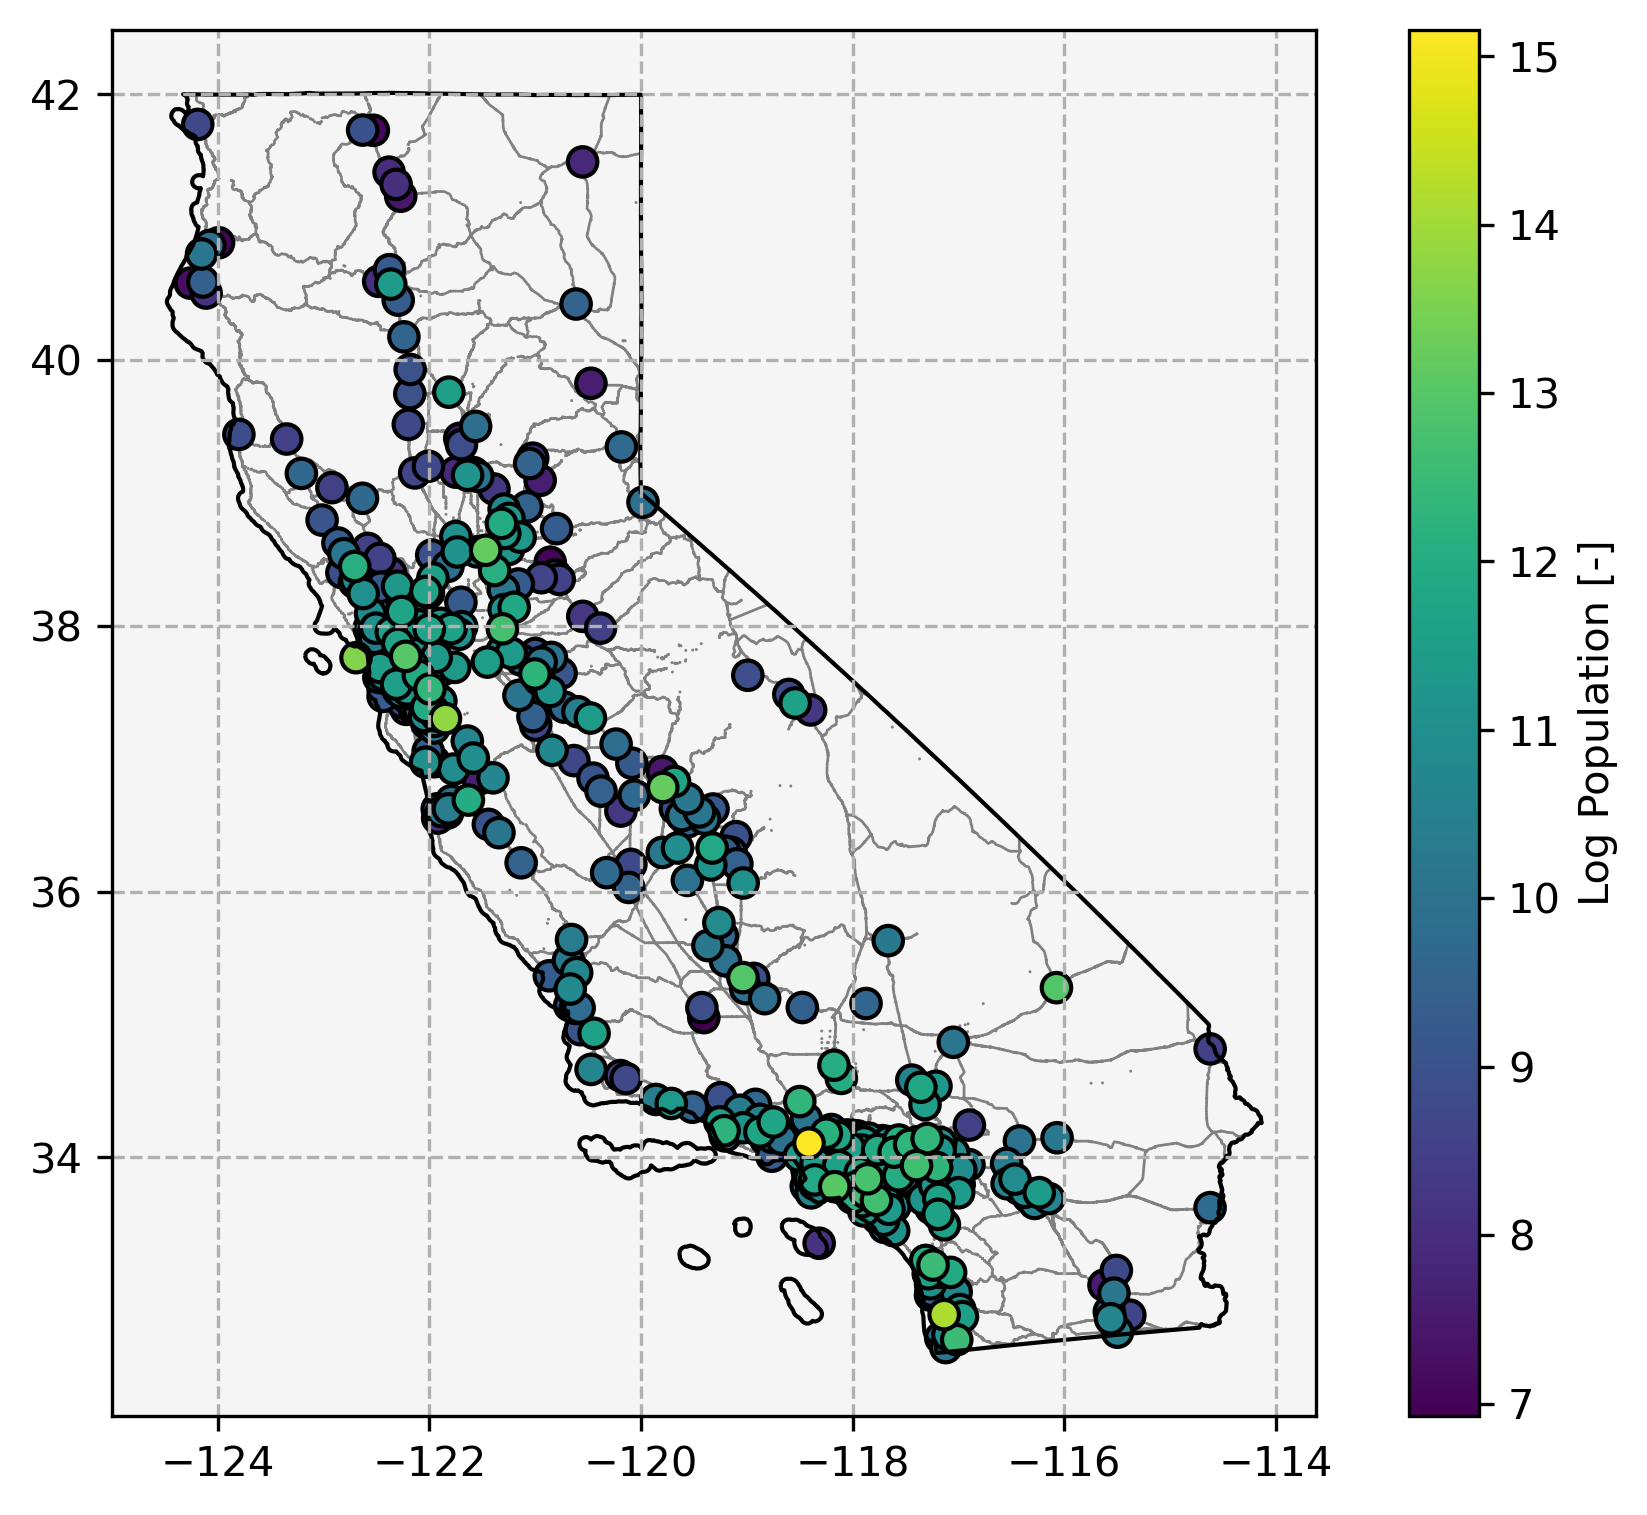
\includegraphics[width = \linewidth]{figs/california_incorporated_places.png}
	\caption{Natural logarithm of population for Incorporated Places in California}
	\label{fig:california_incorporated_places}
\end{figure}

Many of the most heavily populated Places are adjacent with each other or nearly so. The bulk of traffic between these will be local and routine. For the benefit of clarity and brevity these can be merged into super-Places. This is accomplished by the computation of maximally modular communities. First the distances for all pairs are computed. Second an inverse proximity is computed as

\begin{equation}
	\Gamma_{i,j} = \exp{\left(\frac{\Phi_d(i,j)}{\epsilon}\right)}
\end{equation}

where $\epsilon$ is a characteristic distance set at 10 km in this case. Solving for maximally modular communities, centroids of the 34 resulting communities are shown in Figure \ref{fig:california_incorporated_communities}.

\begin{figure}[H]
	\centering
	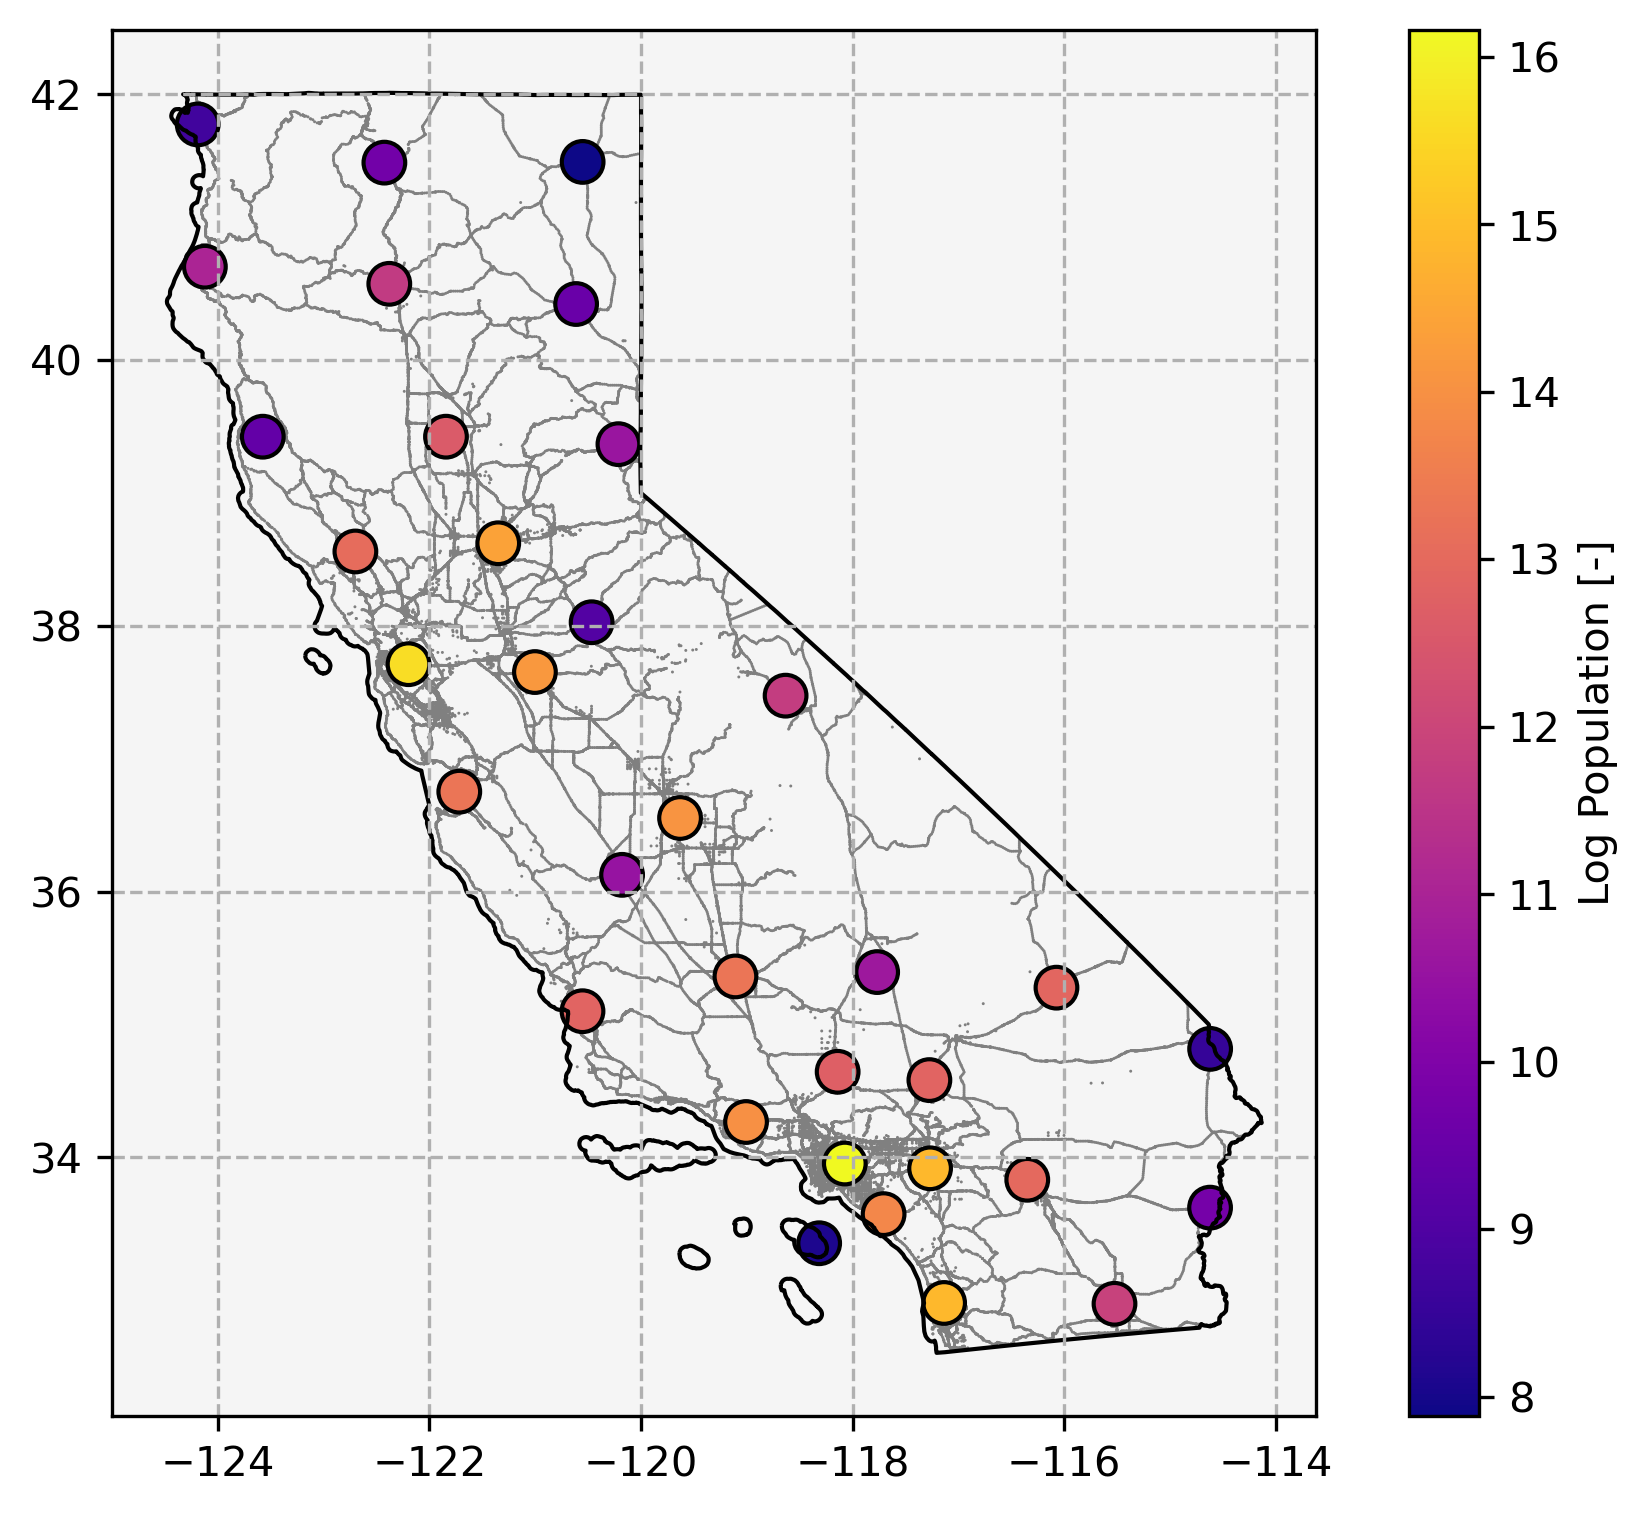
\includegraphics[width = \linewidth]{figs/california_incorporated_communities.png}
	\caption{Natural logarithm  of population for Incorporated Place Communities in California}
	\label{fig:california_incorporated_communities}
\end{figure}

Finally, for the purposes of analysis, points representing departure locations for Phoenix AZ, Las Vegas NV, Reno NV, and Portland/Eugene OR are added to the fringes of the map to represent the associated travel demand.

For long trips, \glspl{bev} will rely on DC charging stations. The locations of all DC charging stations in California are available from AFDC \cite{afdc_2023}. In may 2024 \gls{afdc} listed 2,149 active stations with at least 1 DC charger. This number is somewhat misleading as certain networks report each charger as an individual station even if within line-of-sight of one-another. After merging all stations of the same network which are within 100 meters direct distance of each other the number of stations becomes 1,689. California's DC charging stations include proprietary (vehicle \gls{oem} owned and operated) stations such as Tesla Superchargers and the Rivian Adventure network as well as non-proprietary stations such as those operated by ChargePoint, Electrify America, eVgo, and others. The selected locations and DC charging stations are mapped in Figure \ref{fig:california_stations}.

\end{multicols}

\begin{figure}[H]
\begin{subfigure}{\linewidth/3}
	\centering
	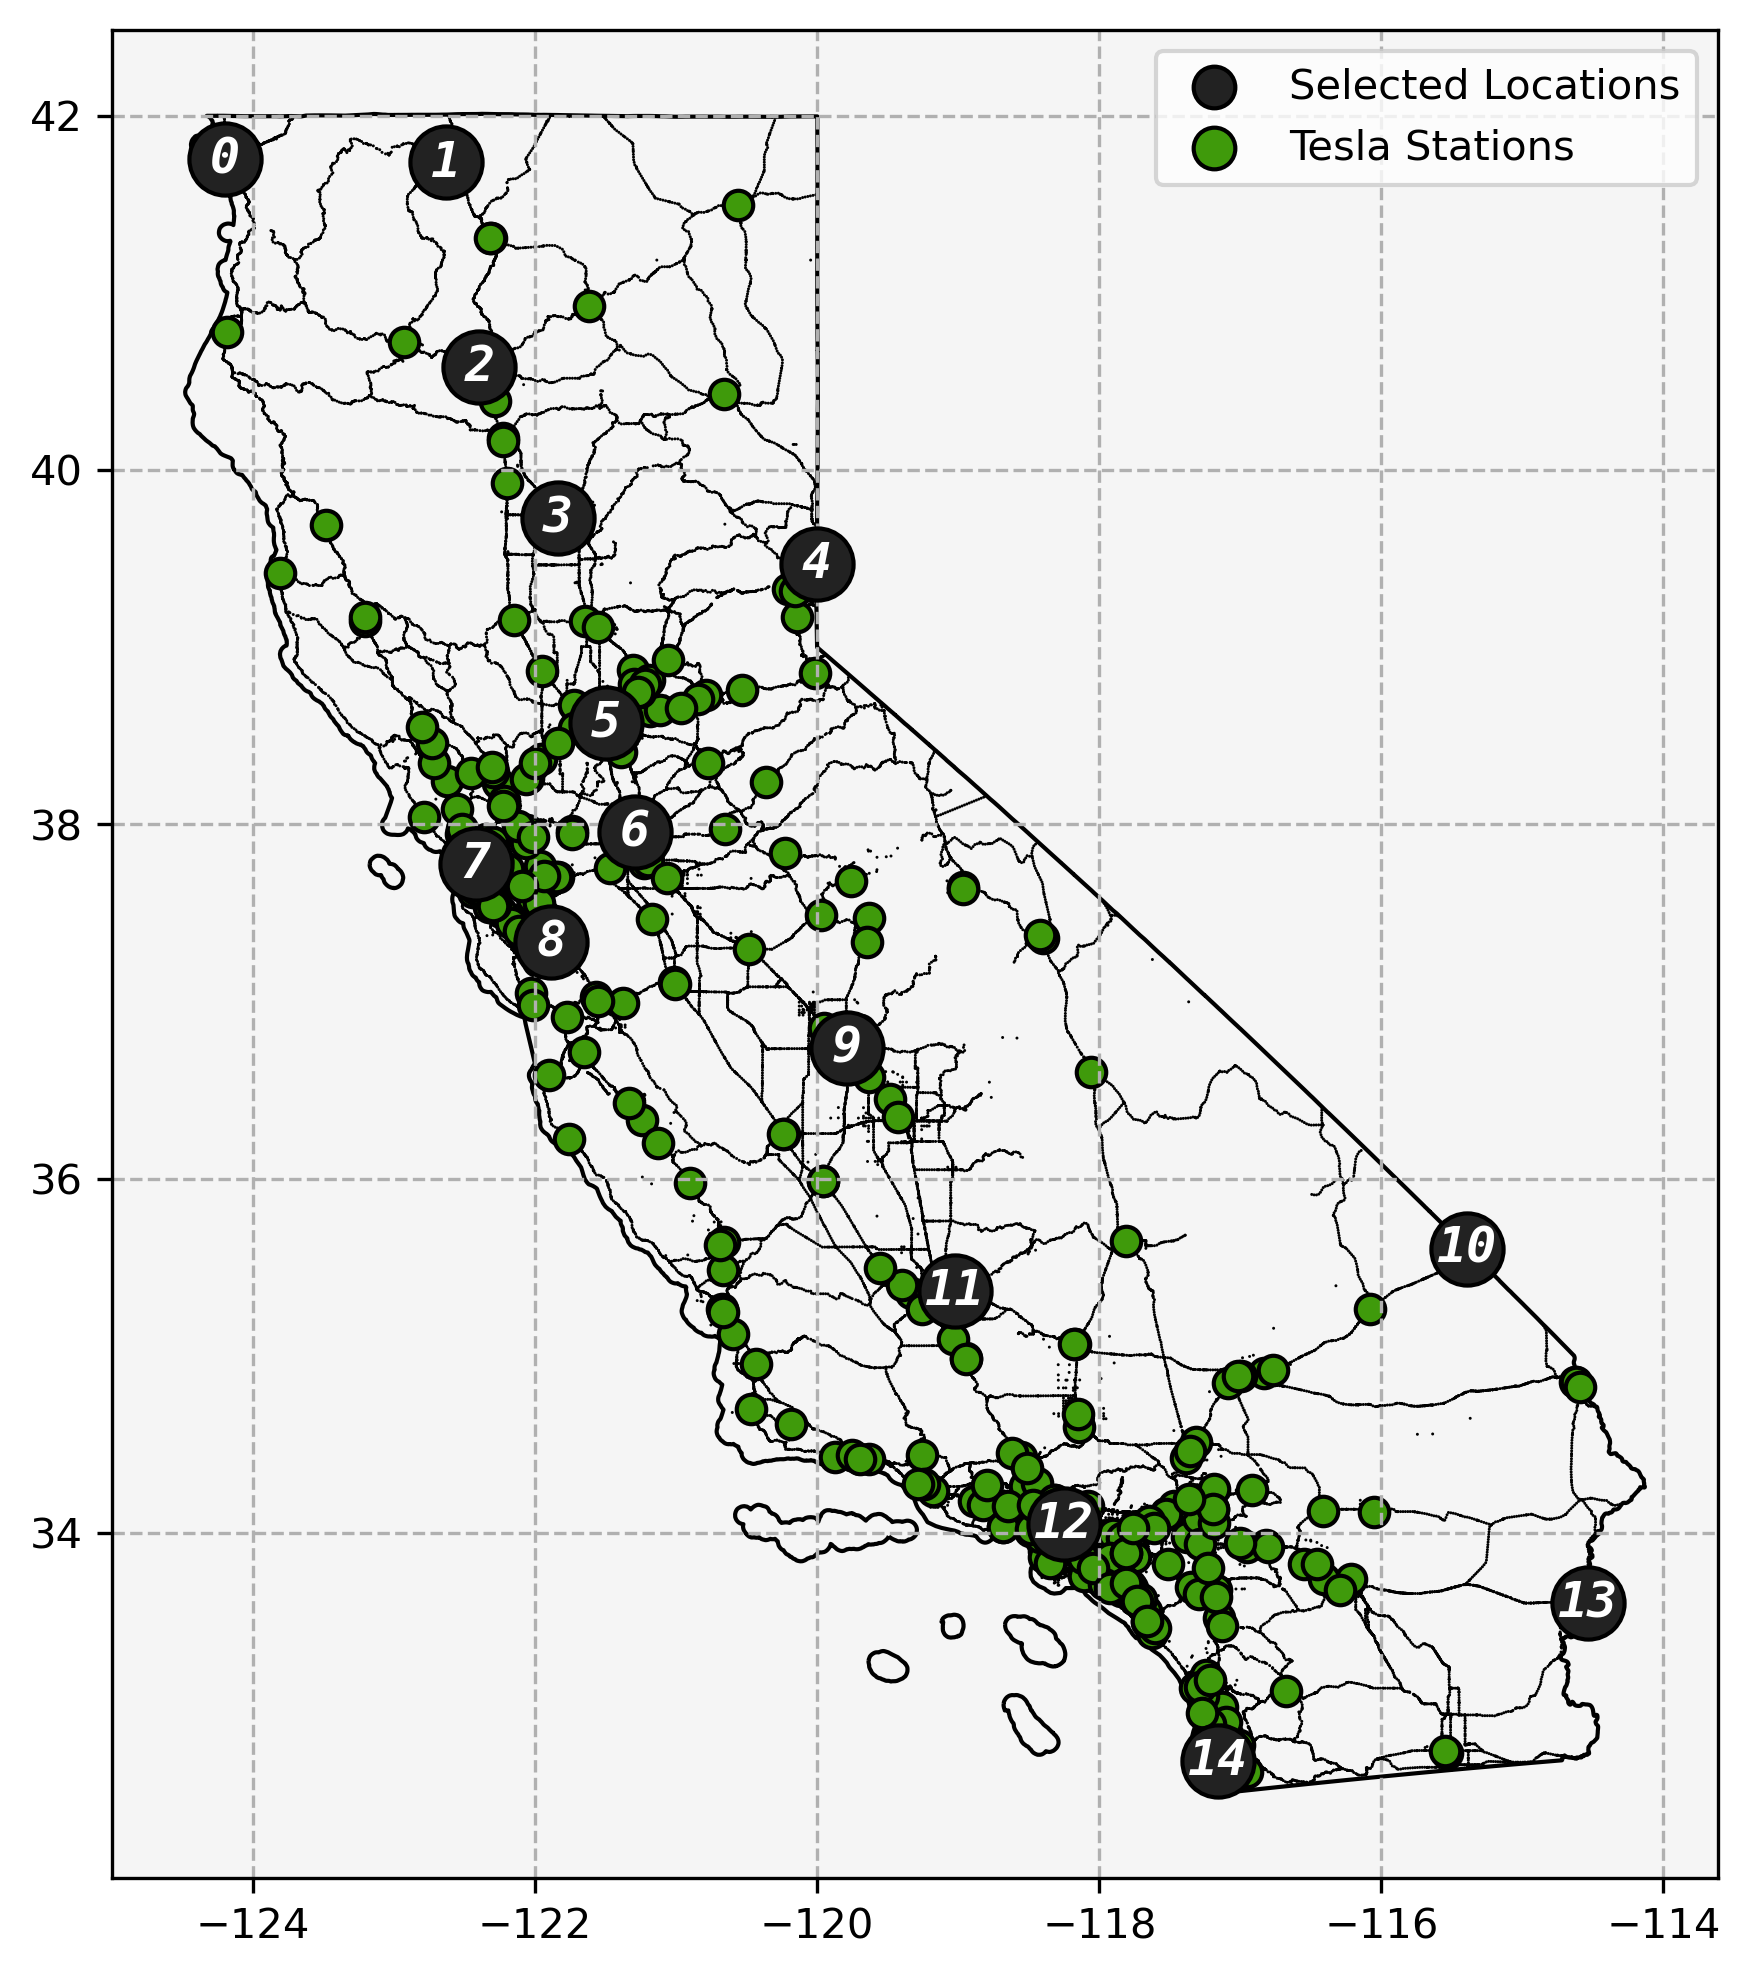
\includegraphics[width = \linewidth]{figs/California_SNG_T.png}
	\caption{Tesla Stations}
\end{subfigure}%
\begin{subfigure}{\linewidth/3}
	\centering
	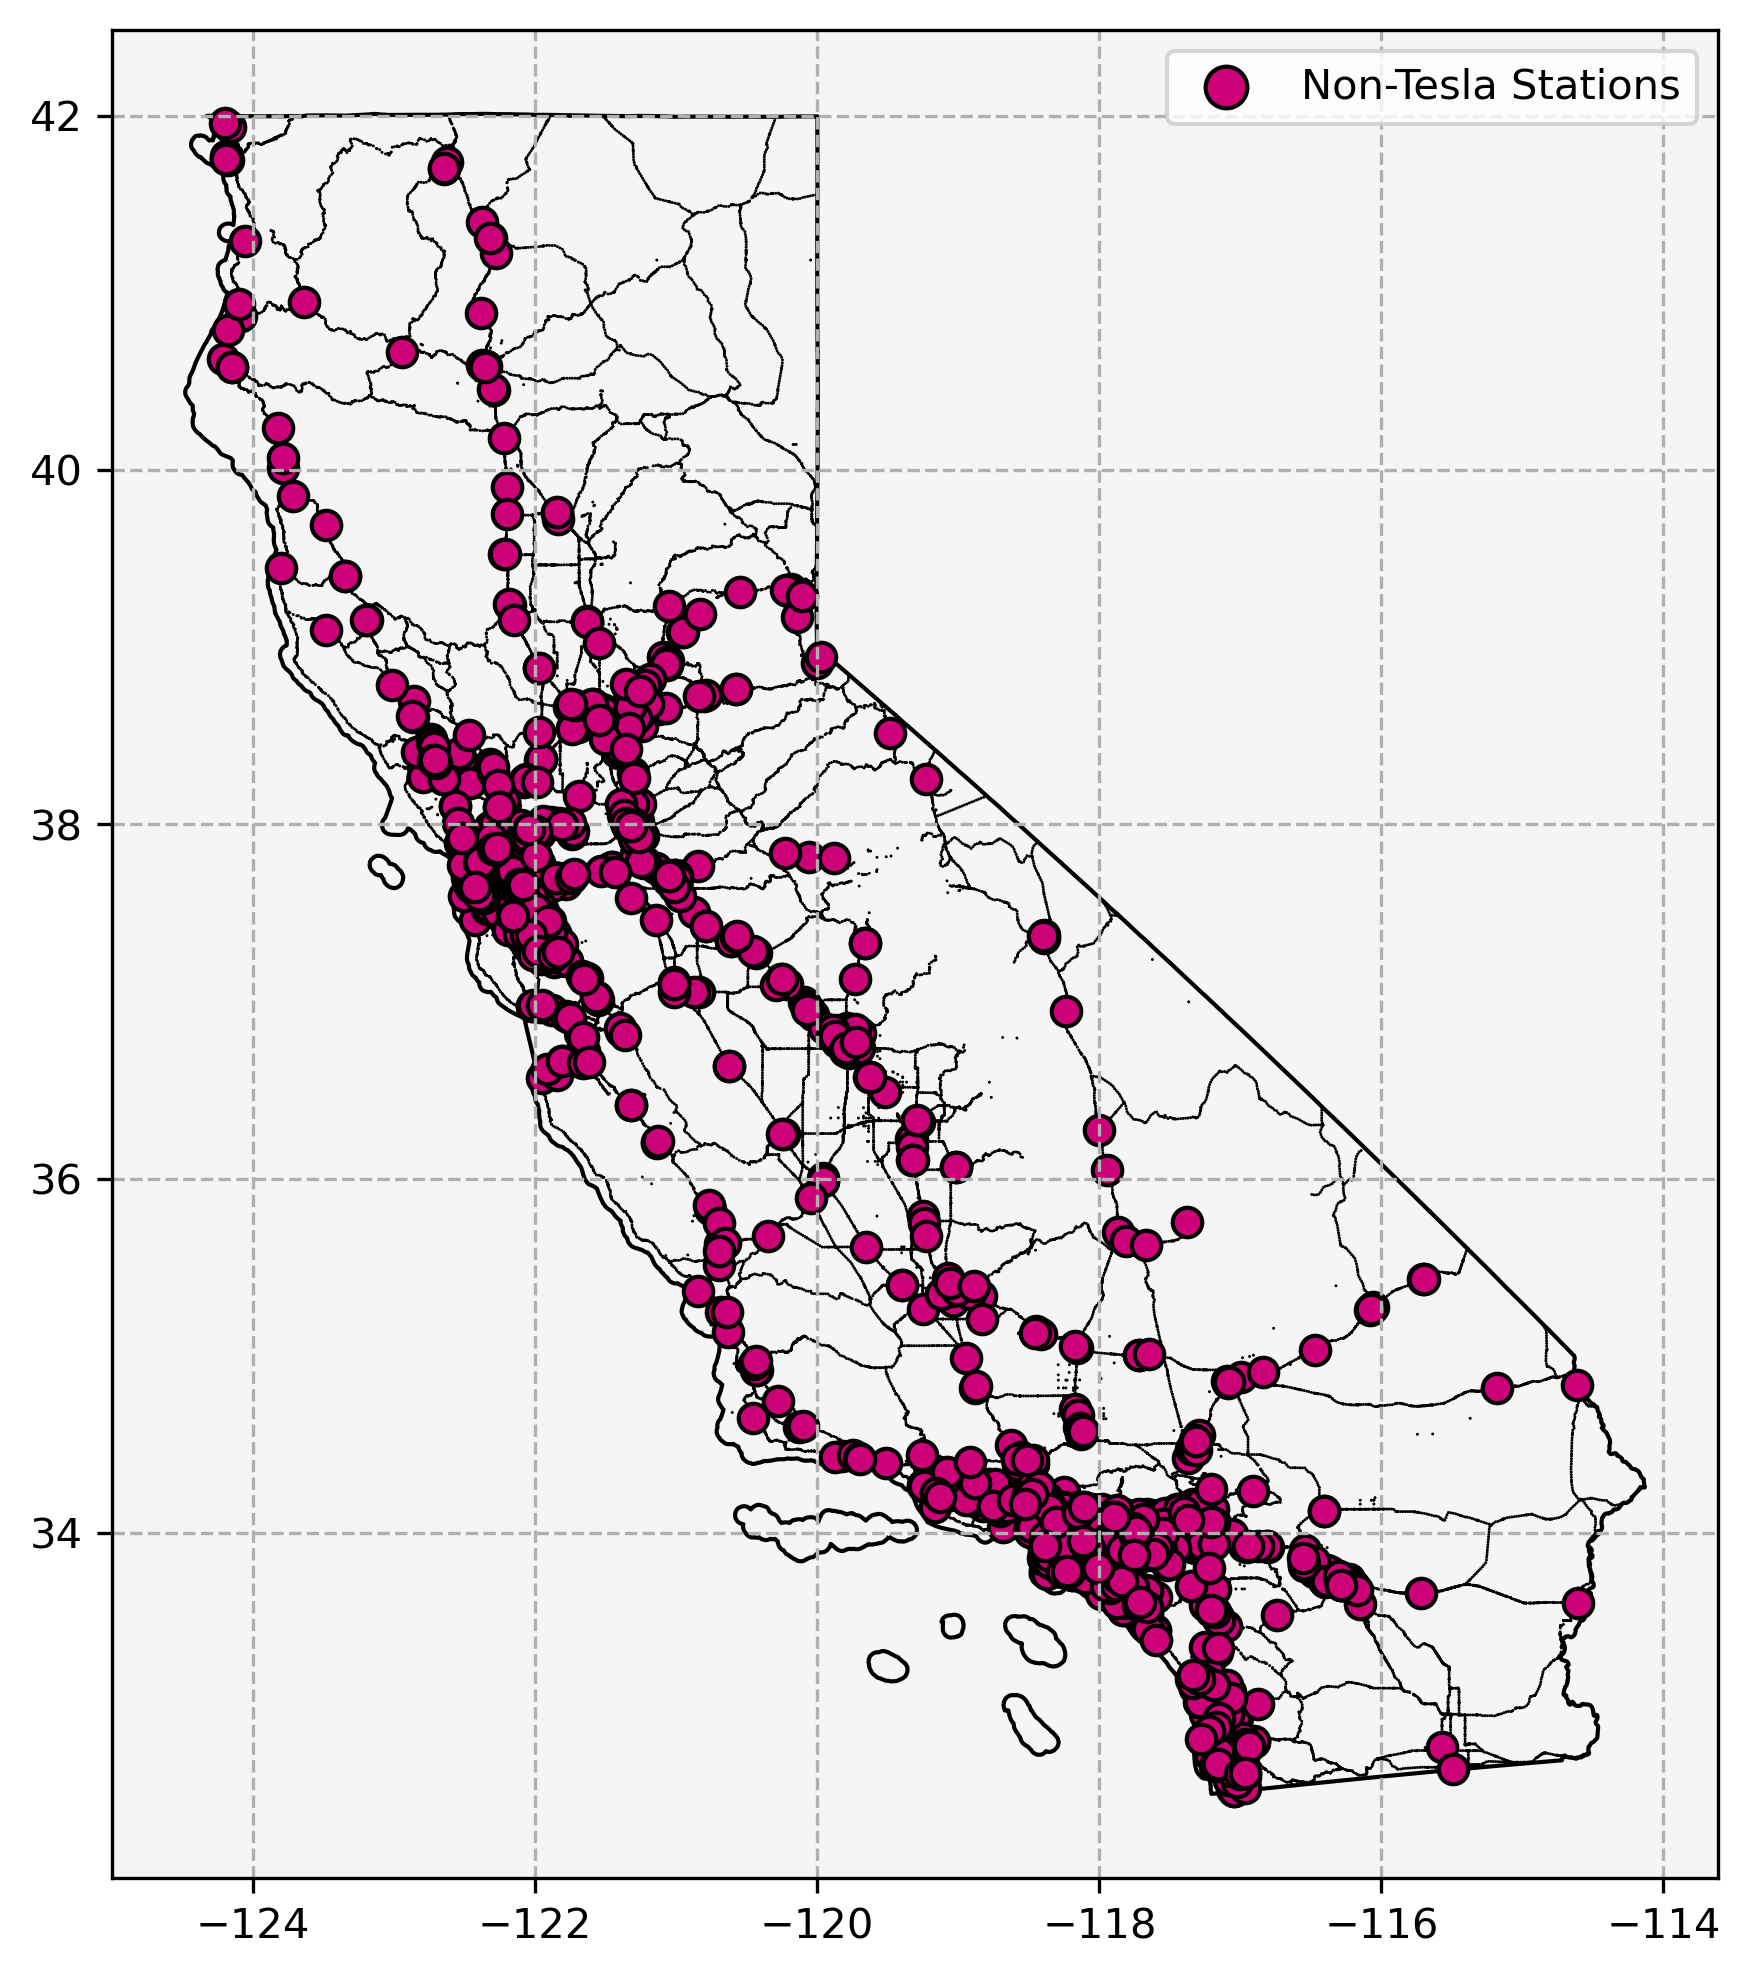
\includegraphics[width = \linewidth]{figs/California_SNG_NT.png}
	\caption{Non-Tesla Stations}
\end{subfigure}
\begin{subfigure}{\linewidth/3}
	\centering
	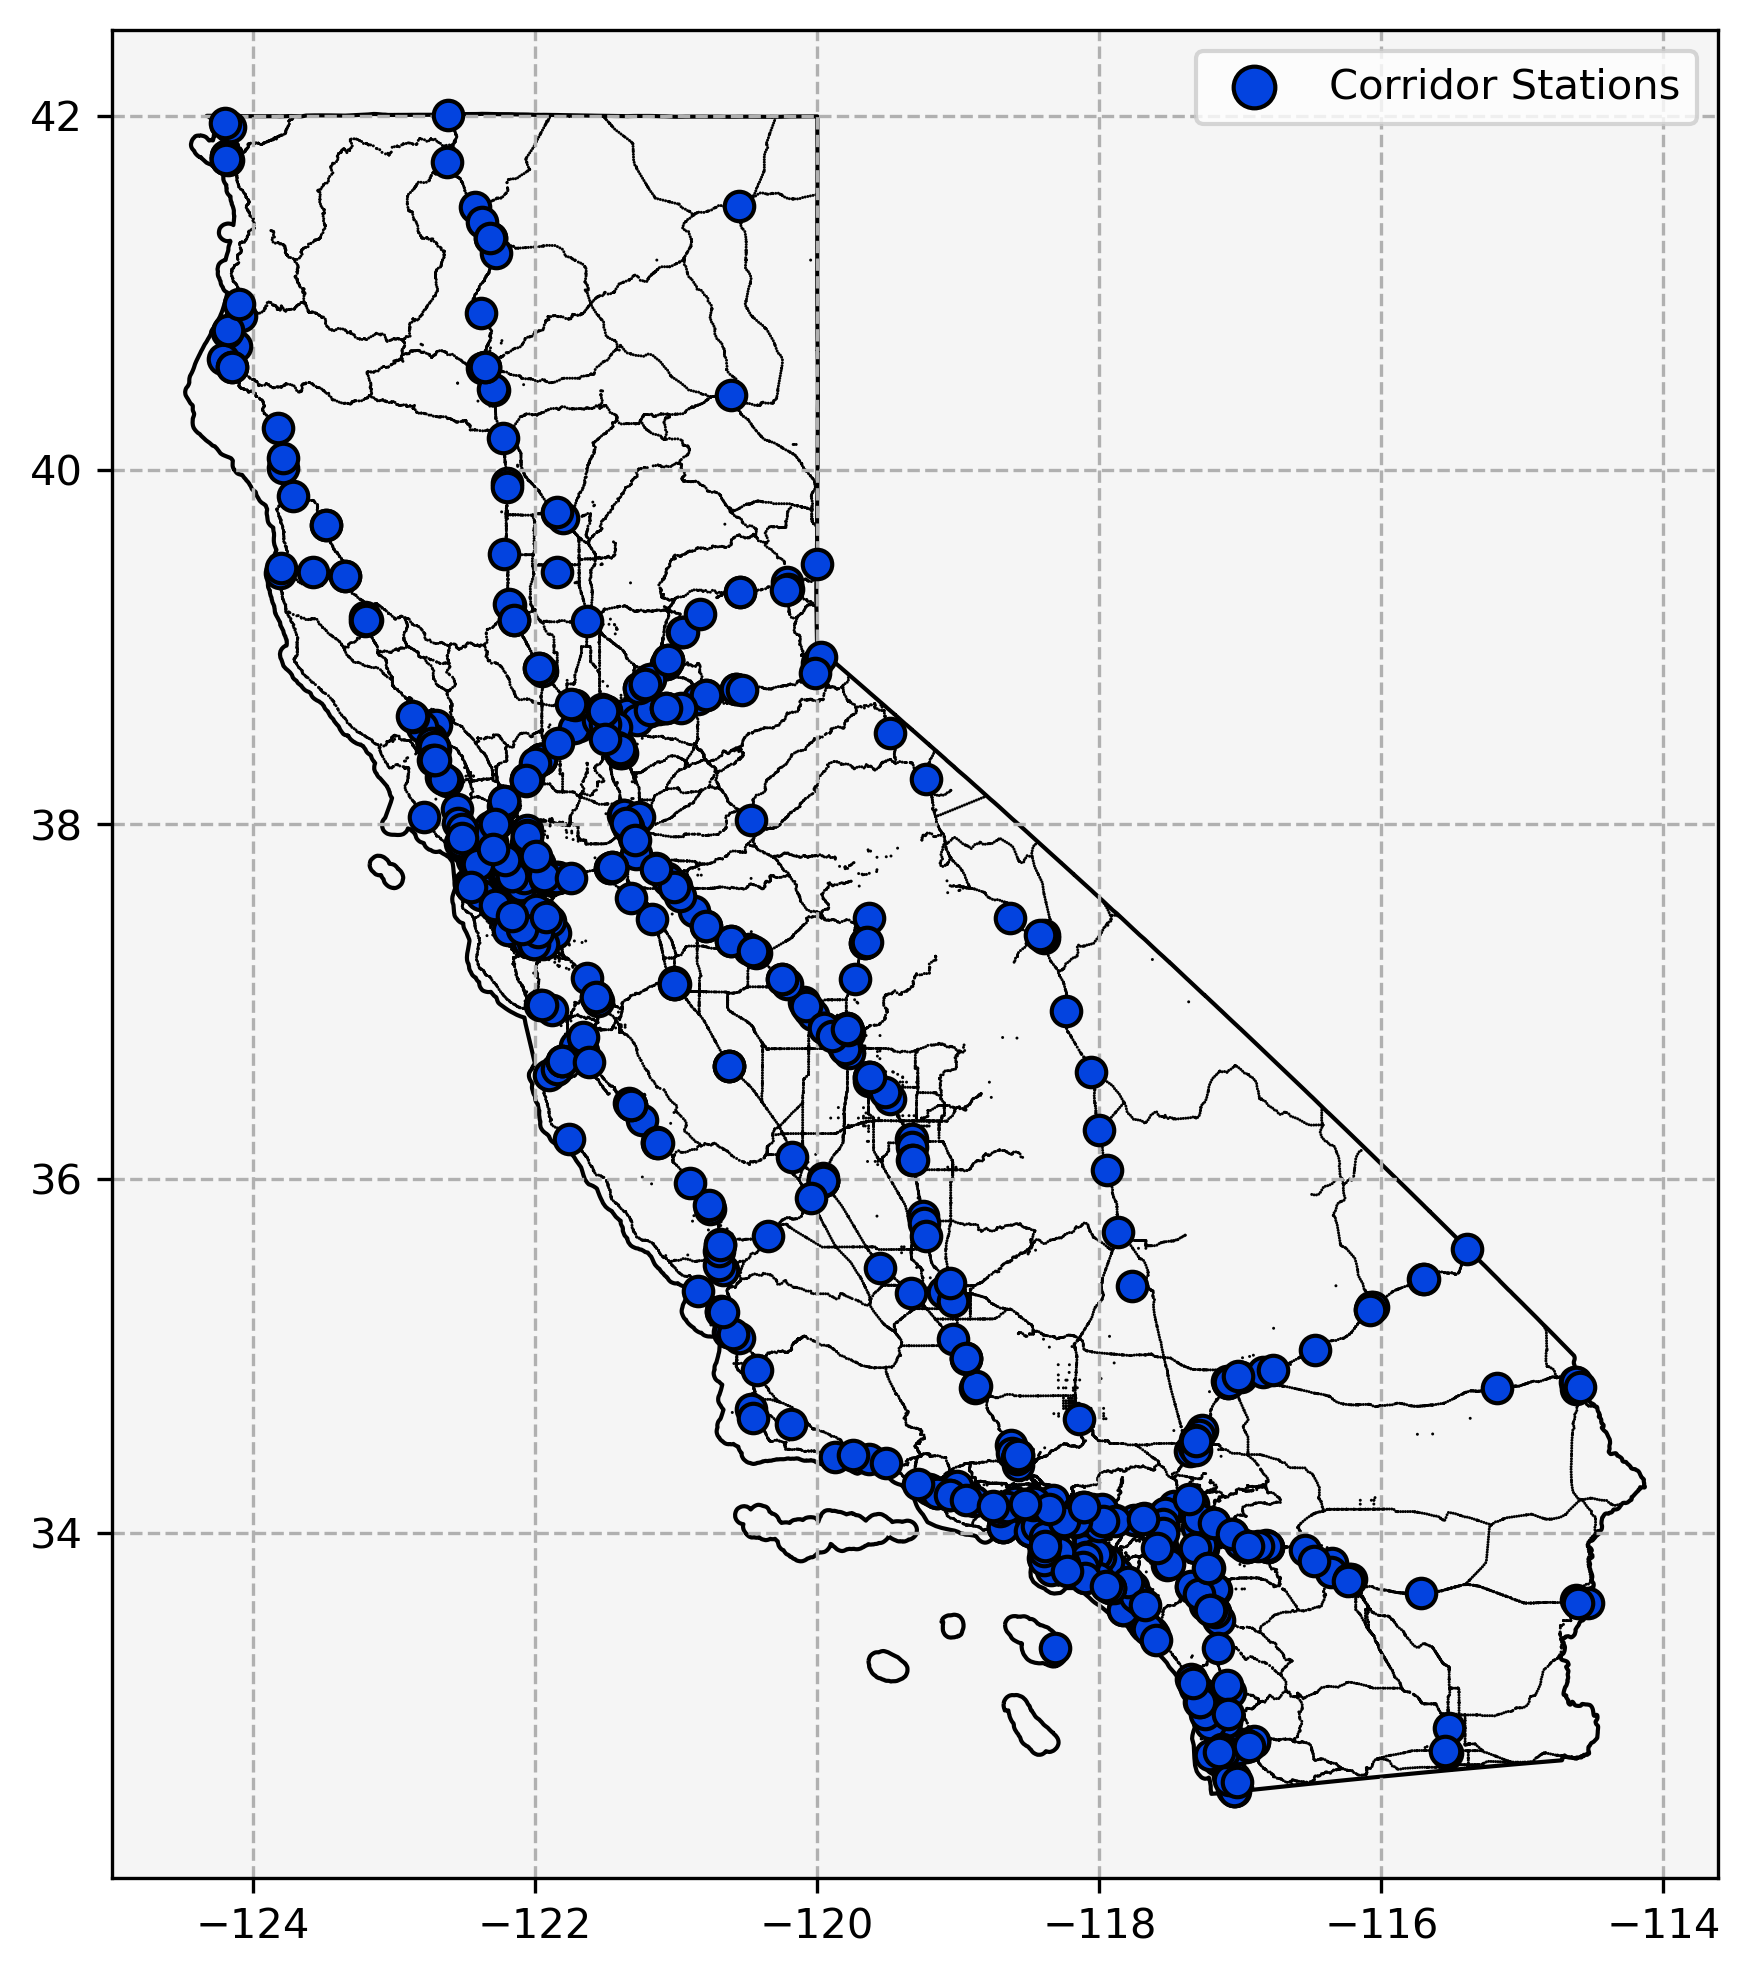
\includegraphics[width = \linewidth]{figs/California_SNG_Corridor.png}
	\caption{Corridor Stations}
\end{subfigure}
\caption{California DC charging stations from \gls{afdc} (May 2024)}
\label{fig:california_stations}
\end{figure}

\begin{multicols}{2}

There are 419 Tesla and 16 Rivian DC charging stations in the state as compared to 1,254 non-proprietary DC charging stations. In practice, many of these stations will be of little use for long distance travel being located far away from primary and secondary roads. Considering only those stations within 1 km of a highway as "corridor" chargers, there are a total of 500 corridor DC charging stations. Of the corridor stations, 156 are Tesla stations, 7 are Rivian stations, and 344 are non-Proprietary stations.

The non-Tesla networks overwhelmingly use CCS or combination CCS/ChaDeMo chargers which reflect the ports on the overwhelming number of non-Tesla \glspl{bev}. By contrast, Tesla chargers and vehicles use the NACS standard. The Tesla and non-Tesla systems are historically separate but increasingly interoperable with the aid of adapters. Tesla drivers use Tesla DC chargers almost exclusively \cite{Visaria_2022}. The Rivian Adventure network is technically interoperable with other J1772 vehicles but is set aside for the exclusive use of Rivian vehicles. The purpose of the Rivian Adventure network serves to allow for Rivian vehicles to charge in remote locations and is not intended to be relied upon exclusively.

The difference between the Tesla DC charging network and the non-Tesla networks extends from function to form. Built out as an investment to entice sales of Tesla vehicles and, until recently, exclusive to them, the Tesla network is technically superior with high maximum charging rates and more greater port usability rates \cite{Rempel_2023, Kozumplik_2022}. The Tesla network is mainly composed of high redundancy stations. Non-proprietary networks have, so far, been utilization and subsidy driven \cite{Gamage_2023} and are widely distributed with low redundancy stations. A stark contrast is seen when examining the ratios of chargers to stations. In California there are 403 Tesla DC charging stations with a total of 7,101 DC chargers for an average of 16.9 chargers per station. Among non-proprietary networks there are a total of 1,254 stations with 4,129 chargers for an average of 3.3 per station. Redundancies for Tesla and non-proprietary networks are shown in Figure \ref{fig:network_histograms}. 


\begin{figure}[H]
	\centering
	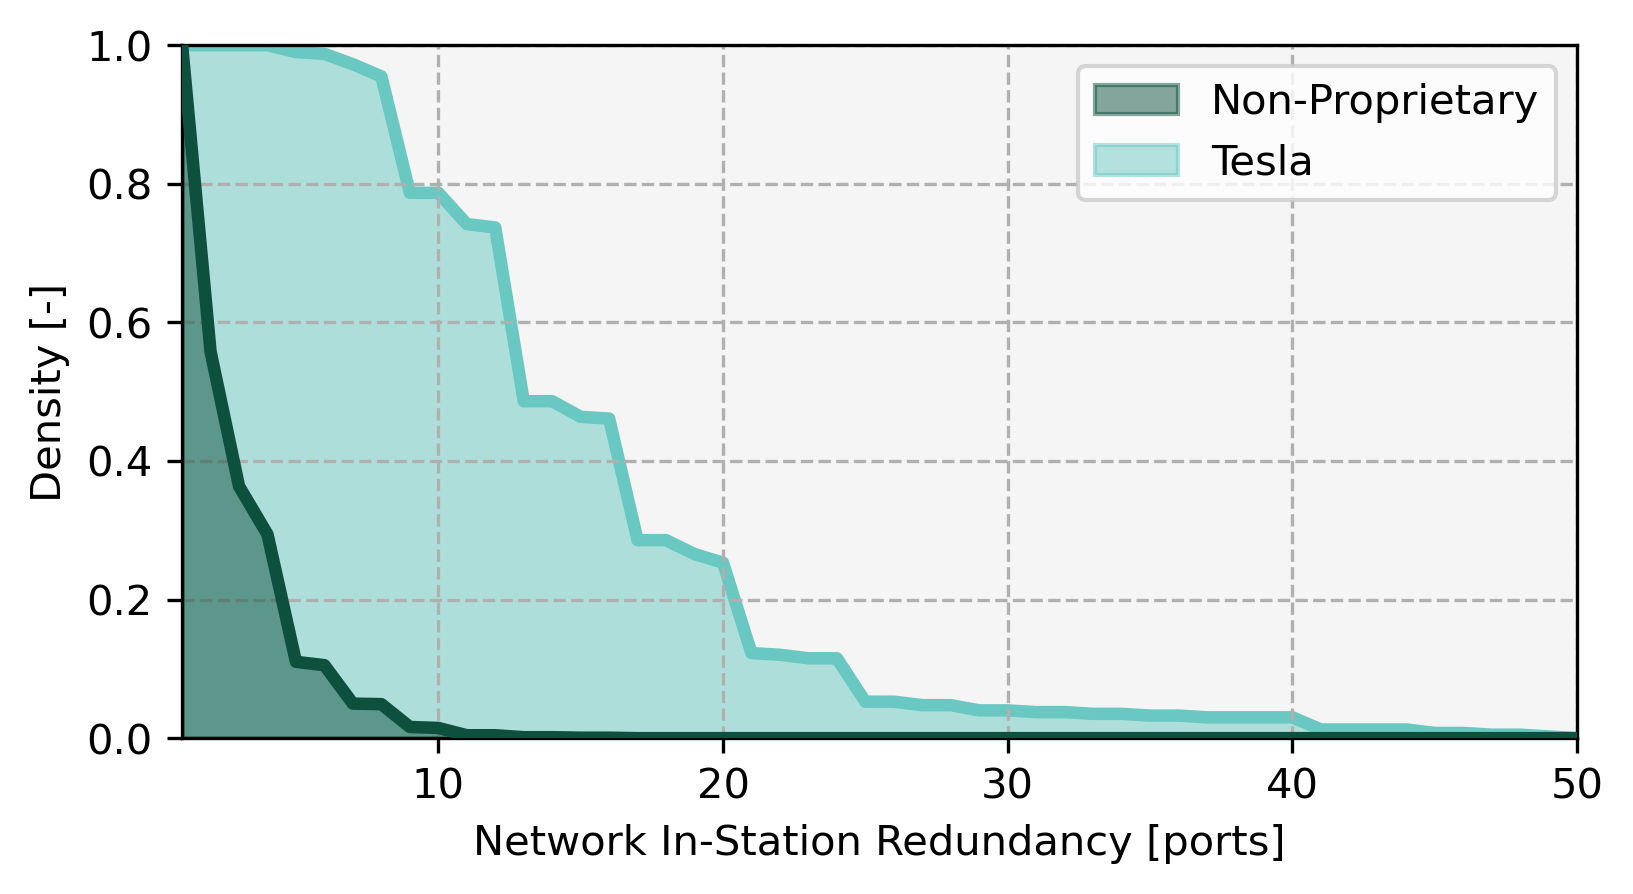
\includegraphics[width = \linewidth]{figs/California_RIS_Hist.png}
	\caption{Survival functions for in-station redundancy for Tesla and other DC charger networks in California}
	\label{fig:network_histograms}
\end{figure}

The Tesla DC charging network develops redundancy primarily in-station where the non-proprietary networks develop redundancy primarily between stations. Non-Tesla chargers are also more likely to be sighted in urban areas suggesting a desire to capture local as well as corridor travel demand. Tesla stations are more often sighted along travel corridors suggesting a focus on enabling long distance travel. In more remote parts of California the proprietary networks nearly match the non-proprietary networks in station numbers. In-station redundancies for DC charging networks in California can be found in Figures \ref{fig:ris_top_networks} and \ref{fig:ris_top_networks_corridor} in the Appendix. Summary statistics for DC charging networks in California can be found in Tables \ref{tab:summary_statistics_afdc} and \ref{tab:summary_statistics_afdc_corridor} in the appendix.

California \glspl{icev} utilize a third and completely separate network of supply stations. There are estimated to be over 8,000 gasoline stations in California \cite{CEC_2022} and these are widely and proportionally distributed. Because no public database for the locations of gasoline stations in the state exists, and due to their ubiquity it is assumed in this study that \gls{icev} driver optimal paths will not be effected by fueling station availability. For this reason, \glspl{icev} are, herein, assumed to take the "direct" path between cities where \glspl{bev} need to find optimal paths on their \glspl{sng}.

\subsection*{Experiment}

In order to understand the effects of vehicular, infrastructural, and behavioral parameters on road-trip accessibility an experiment was carried out on randomly generated combinations. As a baseline, three \glspl{icev} were also modeled. These \glspl{icev} represent different levels of efficiency present in the \gls{icev} fleet. \gls{ess} capacity numbers are pulled from manufacturer websites and energy consumption rates are computed from EPA highway fuel economy ratings \cite{DOE_EPA_2024}. Although substantially less efficient than equivalent \glspl{bev} the comparatively high specific energy of liquid petroleum allows for \glspl{icev} to have higher maximum ranges. \gls{icev} supply infrastructure is modeled to dispense fuel at the normal US rate of 7 gallons per minute which is an equivalent energy supply rate of 14.15 MW. When refueling, the Prius. Golf, and Pacifica, add highway range at rates of 631, 462, and 282 km per minute respectively. The \gls{icev} models and corresponding Regional Impedance values are shown in Table \ref{tab:icev_models}.

\begin{table}[H]
	\centering
	\caption{\gls{icev} models}
	\label{tab:icev_models}
	\begin{tabular}{|C{.45\linewidth}|C{.3\linewidth}|C{.25\linewidth}|}
		\hline Vehicle Model & Parameter & Value \\
		\cline{1-3} & \gls{ess} Capacity & 381 [kWh] \\
		\cline{2-3} & Energy Consumption & 1,346 [kJ/km] \\
		\cline{2-3} 2024 Toyota Prius & Full-Tank Range & 1,018 [km] \\
		\cline{2-3} & California Regional Impedance & 4.131 [hours] \\
		\cline{1-3} & \gls{ess} Capacity & 445 [kWh] \\
		\cline{2-3} & Energy Consumption & 1,839 [kJ/km] \\
		\cline{2-3} 2024 Volkswagen Golf & Full-Tank Range & 871 [km] \\
		\cline{2-3} & California Regional Impedance & 4.151 [hours] \\
		\cline{1-3} & \gls{ess} Capacity & 640 [kWh] \\
		\cline{2-3} & Energy Consumption & 3,015 [kJ/kM] \\
		\cline{2-3} 2024 Chrysler Pacifica & Full-Tank Range & 764 [km] \\
		\cline{2-3} & California Regional Impedance & 4.161 [hours] \\
		\hline
	\end{tabular}
\end{table}

Regional Impedance for \glspl{icev} was computed under the assumption of petroleum supply infrastructure ubiquity. As such, \glspl{icev} were given the "direct" path between locations with stop times added where additional range was needed. For each necessary stop, time was added for refueling to full as well as 10 minutes to divert from the road and handle the transaction prior to refueling. Additionally, drivers of the \glspl{icev} were assumed to keep a 10\% buffer of remaining range. The \glspl{icev} each had similar road-trip accessibility scores of roughly 5.5 hours. The longest arc considered in Crescent City (Location 0) to Phoenix - State Line (Location 13) which is roughly 1,530 km just exceeding double the usable range of the Pacifica. The Prius, Golf, and Pacifica required averages of 0.43, 0.31, and 0.19 supply stops per route respectively.

500 random scenarios were generated by uniform random sampling of the parameters listed in Table \ref{tab:experimental_parameters} and run on three \glspl{sng} as described in \ref{tab:experimental_sngs}. All randomly sampled \glspl{bev} in this study are assumed to have an energy consumption rate of 608 kJ/km this being the EPA energy consumption rate of a Tesla Model 3 in highway operation \cite{DOE_EPA_2024}. Highway operation is assumed herein due to the focus on long trips. Thus \gls{bev} full-charge ranges will be between 237 and 711 km. Vehicles are assumed to fast charge only up to 80\% \gls{soc} in order to remain in the constant current range. When charging, sampled \glspl{bev} add highway range at a rate between 4.9 and 19.7 km per minute. Risk attitude was modeled as in \eqref{eq:superquantile} with the range centered around the mean parameter $\overline{p}$ where $p_0 = \overline{p} - .1$ and $p_1 = \overline{p} + .1$. 

\begin{table}[H]
	\centering
	\caption{Parameters and ranges for experiment.}
	\label{tab:experimental_parameters}
	\begin{tabular}{|C{\linewidth/2}|C{\linewidth/2}|}
		\hline Parameter & Range \\
		\hline \gls{ess} Capacity & [40 kWh, 120 kWh] \\
		\hline \gls{ess} Max Charge Rate & [50 kW, 200 kW] \\
		\hline Driver Risk-Attitude Mean & [.1, .9] \\
		\hline \gls{evse} Reliability & [.5, 1] \\
		%		\hline Station Arrival Ratio Mean & [1, 3] \\
		\hline
	\end{tabular}
\end{table}

\begin{table}[H]
	\centering
	\caption{\glspl{sng} used in experiment.}
	\label{tab:experimental_sngs}
	\begin{tabular}{|C{\linewidth/3}|C{\linewidth*2/3}|}
		\hline Label & Networks Included \\
		\hline Combined & All stations \\
		\hline Tesla & Only Tesla stations \\
		\hline Non-Tesla & All non-Tesla stations \\
		\hline
	\end{tabular}
\end{table}

Outputs were processed to compute a population weighted Regional Impedance as in \eqref{eq:regional_impedance}. Impedance was selected as the metric of evaluation rather than accessibility as travel demand for each arc was the same for all cases. Linear regression was performed on the results of the random experiment. Using as output, the neutral expectation of road-trip accessibility for each of the 500 randomly sampled vehicles on each of the \glspl{sng}. Significant parameters from the regression are shown in Figure \ref{fig:significant_parameters}.

\begin{figure}[H]
	\centering
	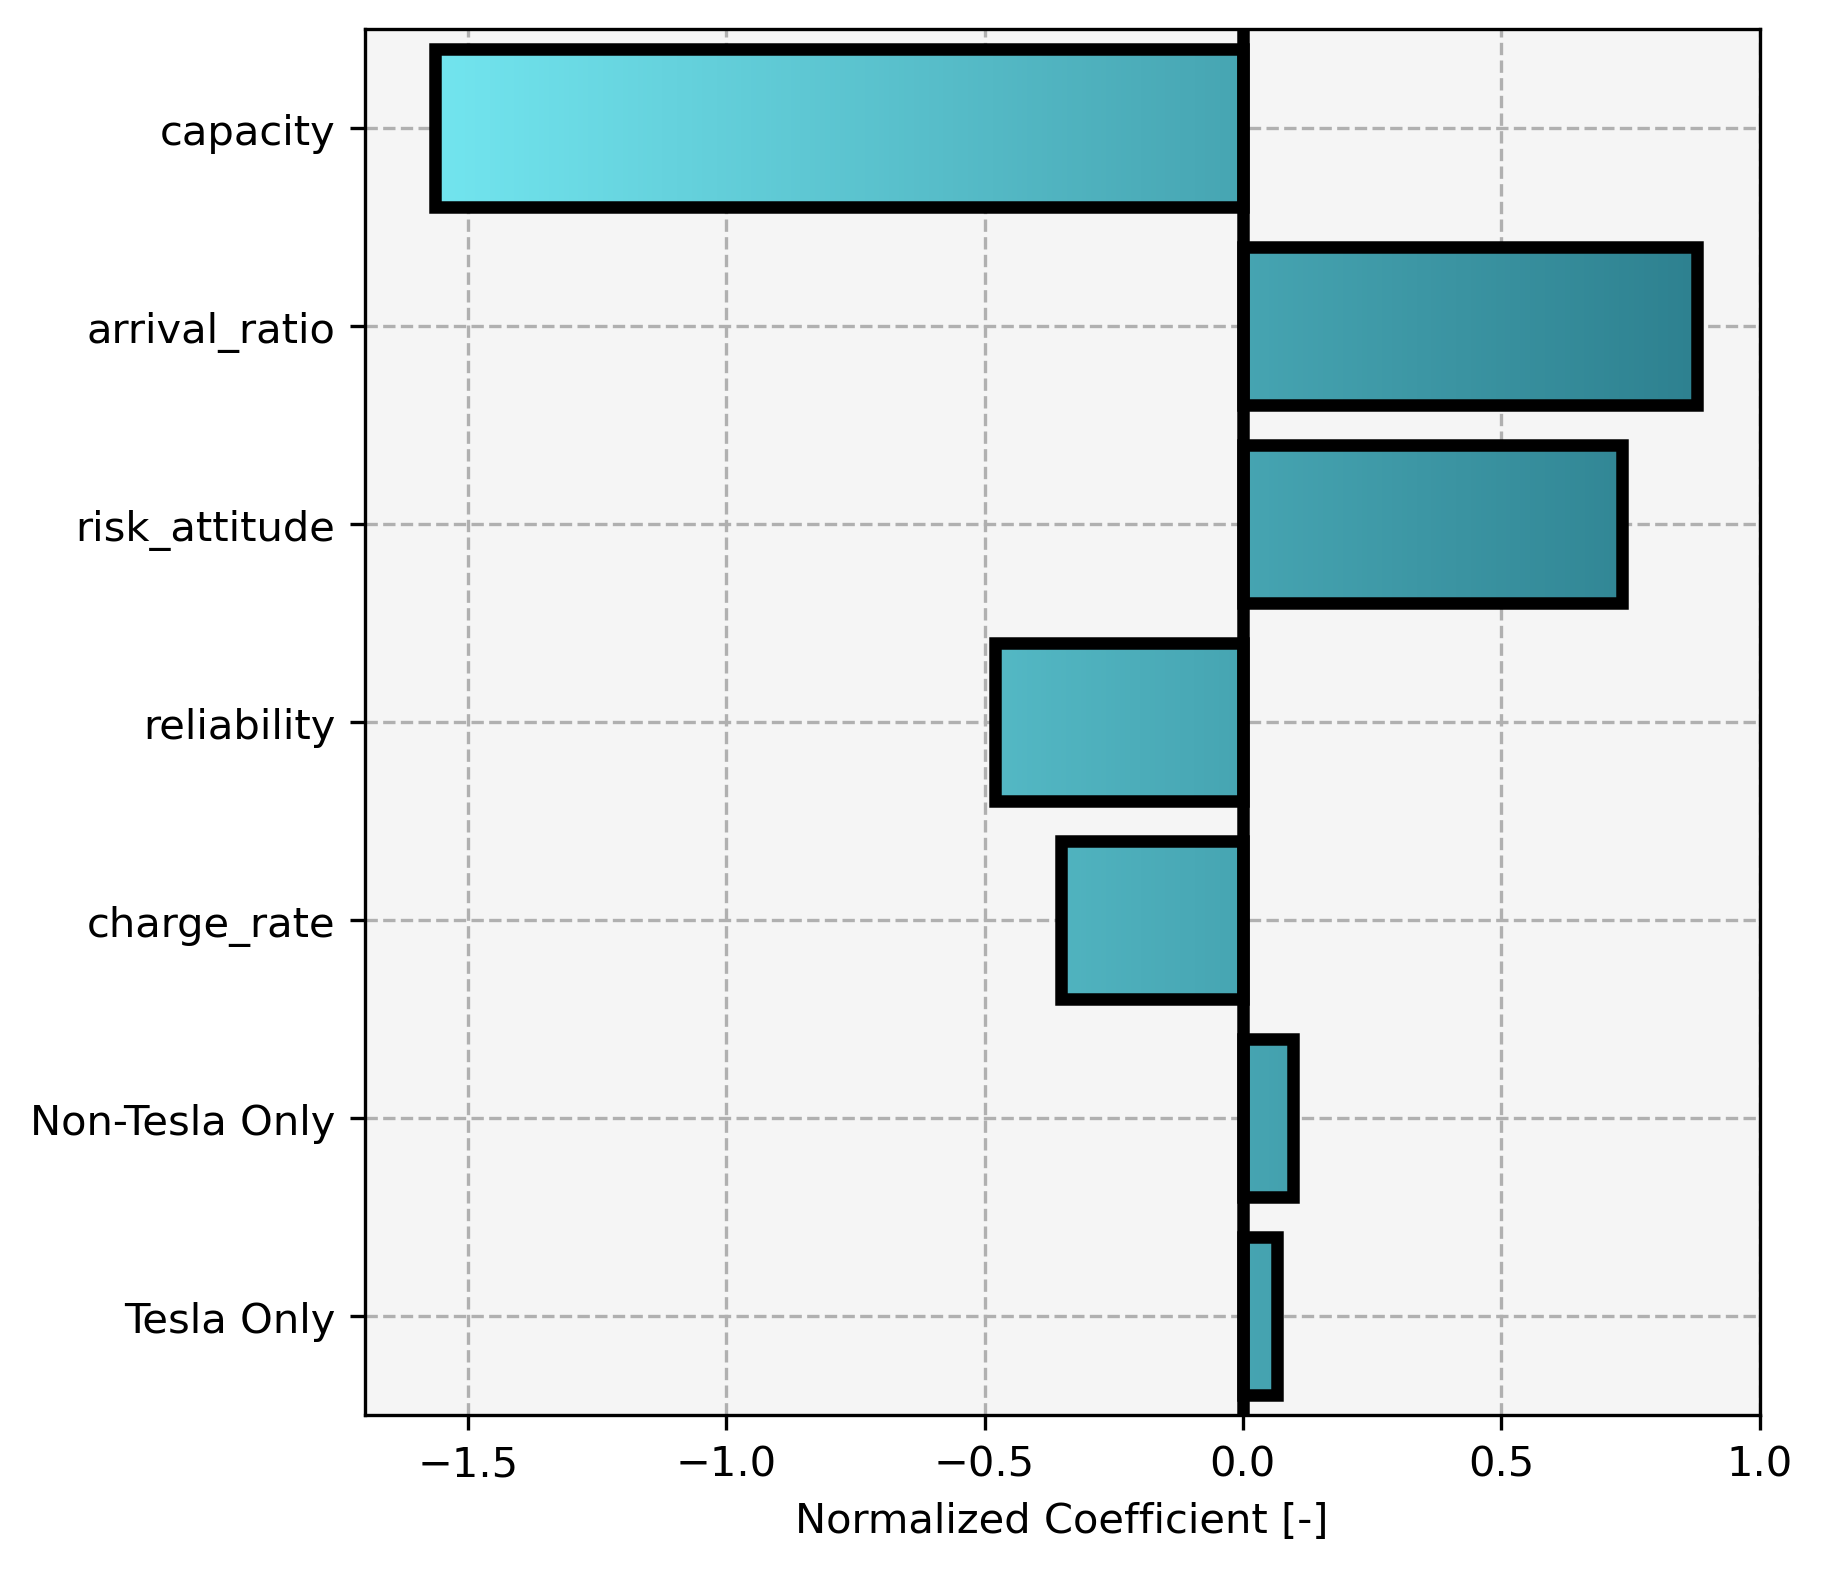
\includegraphics[width = \linewidth]{figs/significant_parameters.png}
	\caption{Coefficients for significant parameters from linear regression}
	\label{fig:significant_parameters}
\end{figure}

Regression details are provided in Tables \ref{tab:regression_anova} and \ref{tab:regression_coefficients} in the Appendix. The regression analysis shows that vehicular, infrastructural, and behavioral parameters have significant impacts on road-trip accessibility. The vehicular parameters of capacity and charge rate have the predictable effect of reducing expected travel times. Capacity being the more more important parameter is explicable as higher capacity vehicles offer the ability to stop less frequently. Saving an entire charging event can be very impactful in a region the size of California. Among the infrastructure parameters, higher reliability contributed to lower travel times where higher arrival ratios contributed to higher travel times. Both reliability and arrival ratio primarily effect queuing times as, even with 50\% equipment reliability, most stations have sufficient redundancy to guarantee at least one operational charger. The range of arrivals ratios considered goes from normal to swamped and long queues can be expected for high arrival ratios even at high redundancy stations. Risk attitude was also significant in determining outcomes as those drivers with more cautious risk attitudes will tend to maintain higher \gls{soc} and utilize more reliable and redundant routes. finally, access to the entire network is better than restriction to just part of it but being restricted to only Tesla stations should be slightly less damaging than access to only non-Tesla stations. Boxplots of expected travel times are shown in Figure \ref{fig:networks_boxplots}.

\begin{figure}[H]
	\centering
	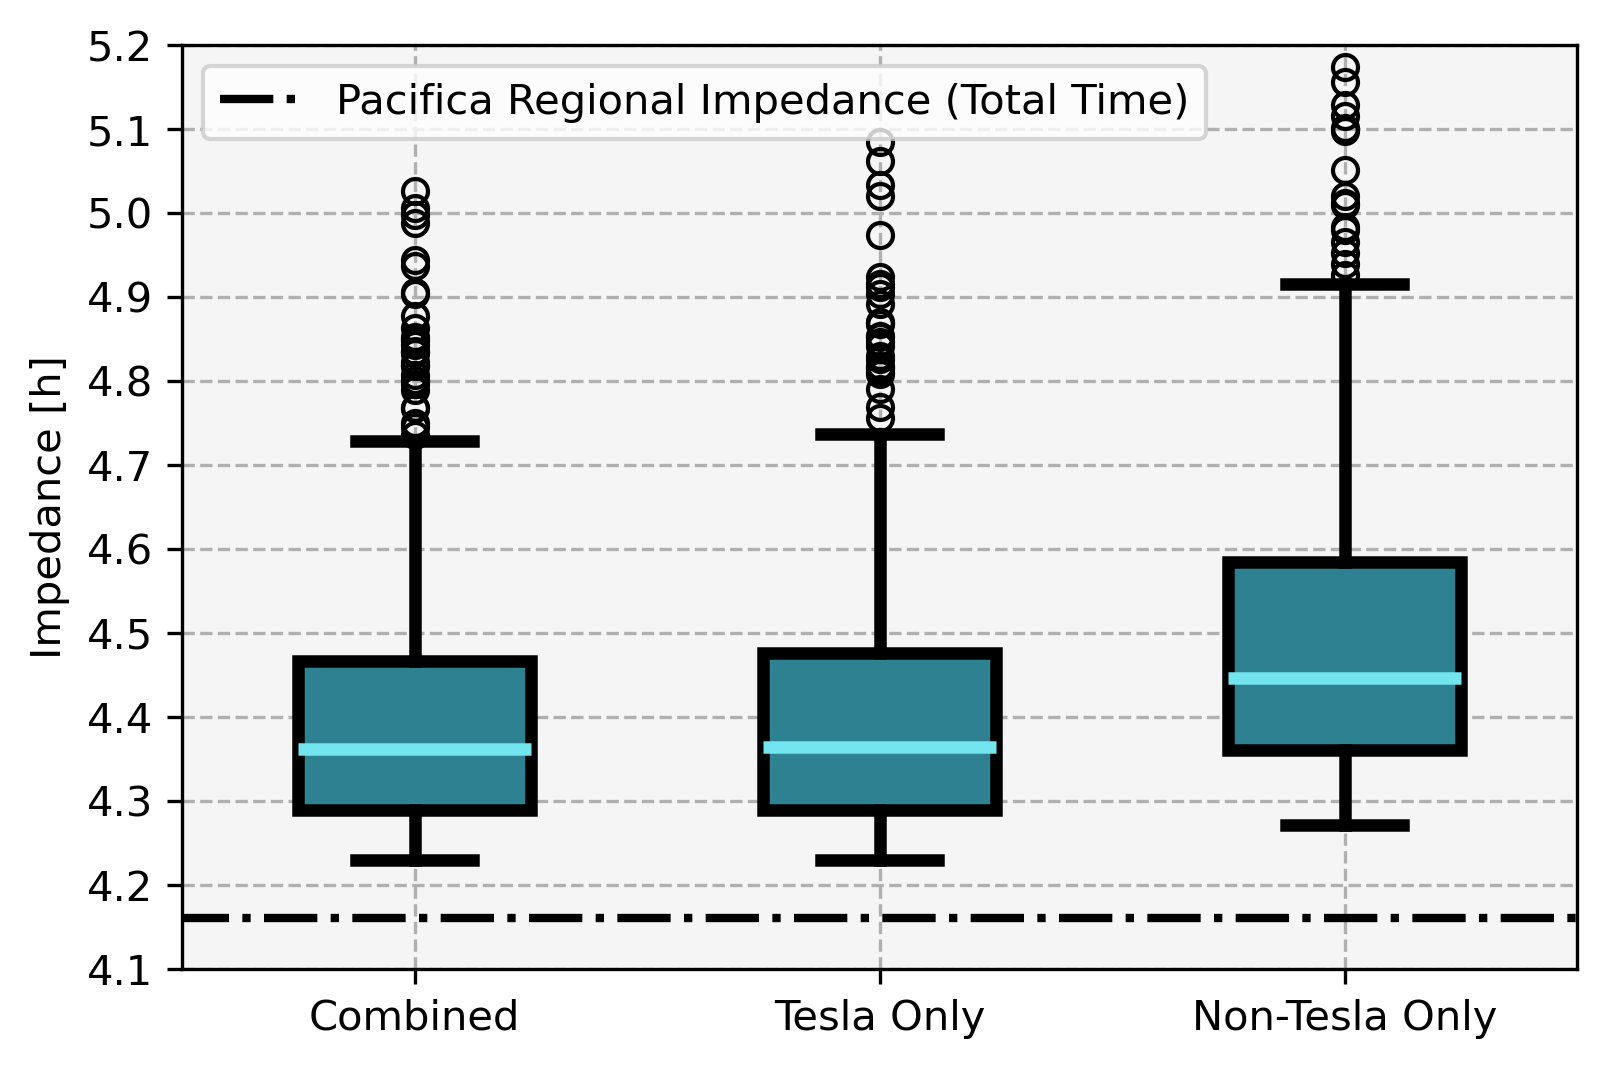
\includegraphics[width = \linewidth]{figs/Networks_Boxplots_Weighted_Impedance.png}
	\caption{Boxplots of experiment outputs by \gls{sng}}
	\label{fig:networks_boxplots}
\end{figure}

While the differences between the \glspl{bev} on the basis of \gls{sng} access are observed to be slight, the differences between the means of each and the worst of the \glspl{icev} is quite large. The difference is roughly 45 minutes much of which can be explained by the shorter ranges and longer supply times inherent to the \glspl{bev}. In the best of circumstances, \glspl{bev} can reach near parity with \glspl{icev}. However, \glspl{bev} impedance will, nearly always, be substantially higher than \gls{icev} impedance due to the necessity of charging events. Some will argue that this difference is unimportant as \gls{bev} drivers can charge their vehicles while stopping for meals or during other natural breaks. This logic has been used to show that \glspl{bev} may approach convenience parity with \glspl{icev} in reasonable circumstances \cite{Dixon_2020}. However, where such long breaks are optional for \gls{icev} drivers, they are mandatory for \gls{bev} drivers and must be taken at specific points throughout the trip to coincide with charging. This loss of optionality must be accounted an inconvenience even for drivers who accustomed to long breaks.

Most of the difference in impedance is due to charging and queuing times while only a small part is due to route alterations. Isolating the driving times by subtracting supply and setup times, the differences between \glspl{bev} and \glspl{icev} \glspl{sng} are substantially smaller than those in total trip time as shown in Figure \ref{fig:networks_boxplots_driving}. It should, however, be noted that there is a long tail on the driving time distributions due to the occasional need to take a significantly altered route to confidently reach a remote destination.

\begin{figure}[H]
	\centering
	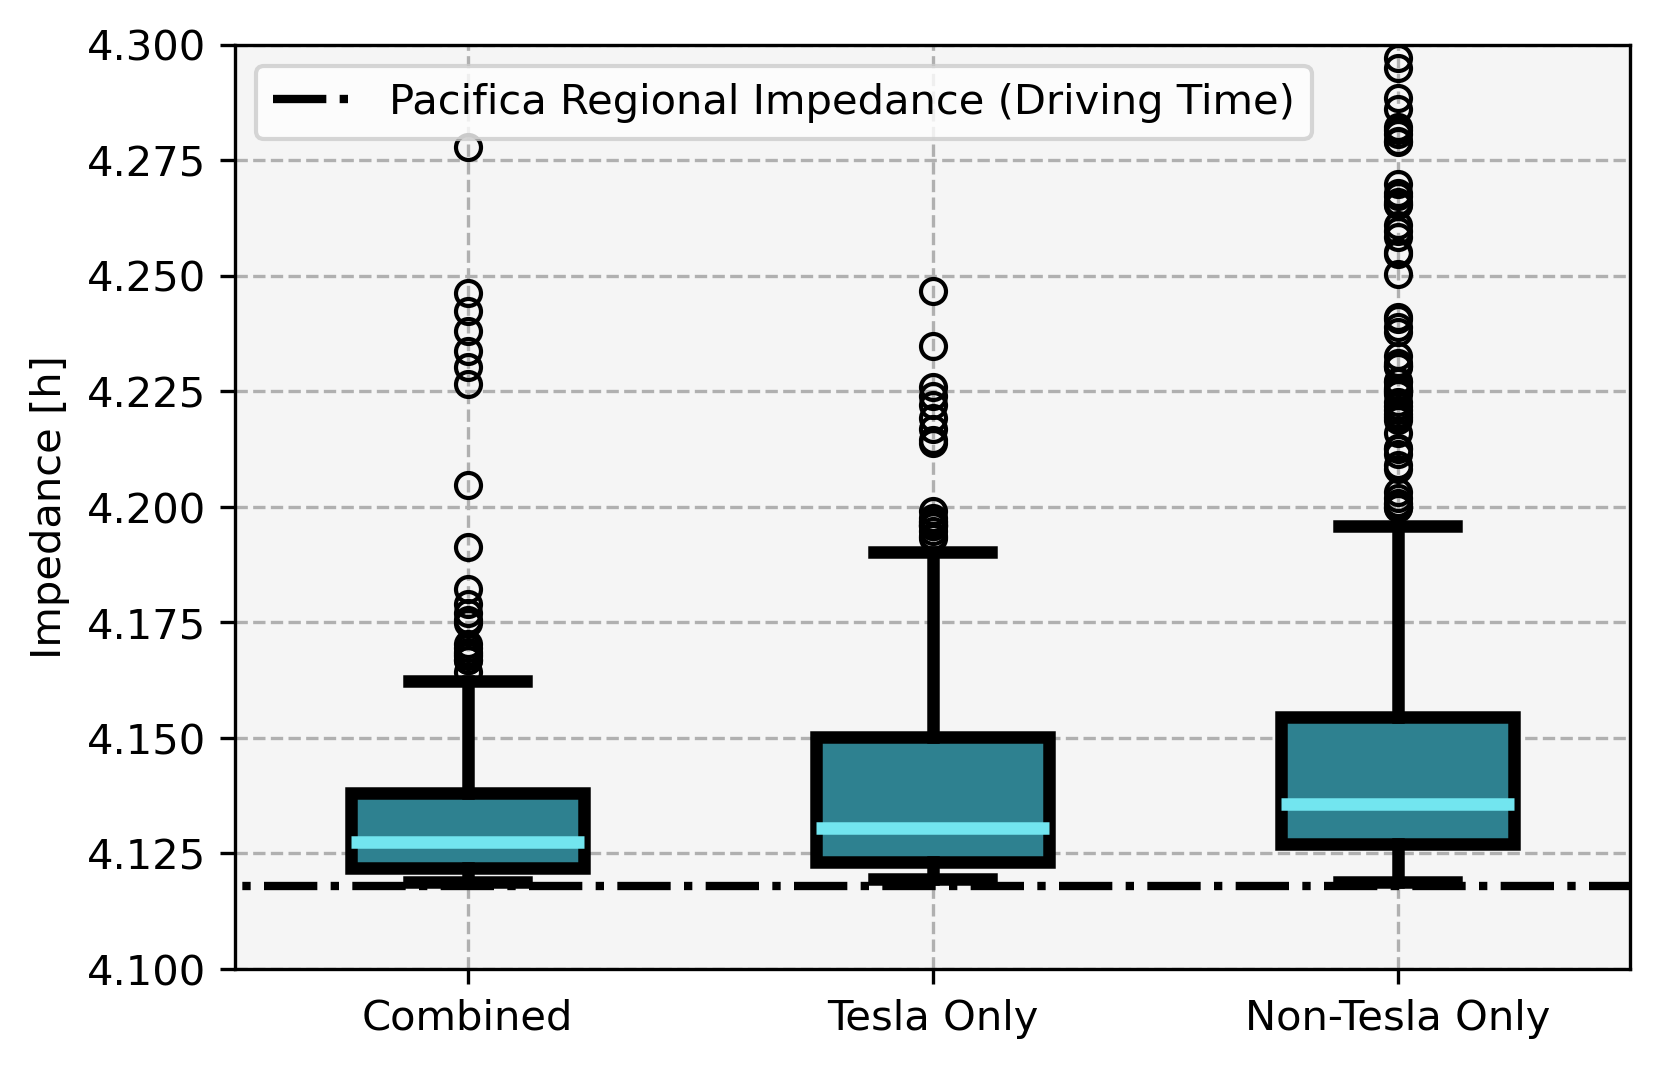
\includegraphics[width = \linewidth]{figs/Networks_Boxplots_Weighted_Impedance_Driving.png}
	\caption{Boxplots of experiment outputs by \gls{sng} (driving time only)}
	\label{fig:networks_boxplots_driving}
\end{figure}

Different parts of the state will have different experiences. Residents of large population centers which are proximate to other large population centers will expect to have lower travel needs than those in more remote areas. In general, the impedance disparities associated with different vehicular, infrastructural, and behavioral characteristics will also scale with impedance. As California is a large state with a diversity of land use and road infrastructure volume, there is a pronounced difference in Specific Regional Impedance as shown in Figure \ref{fig:networks_boxplots_locations}.

\end{multicols}

\begin{figure}[H]
\centering
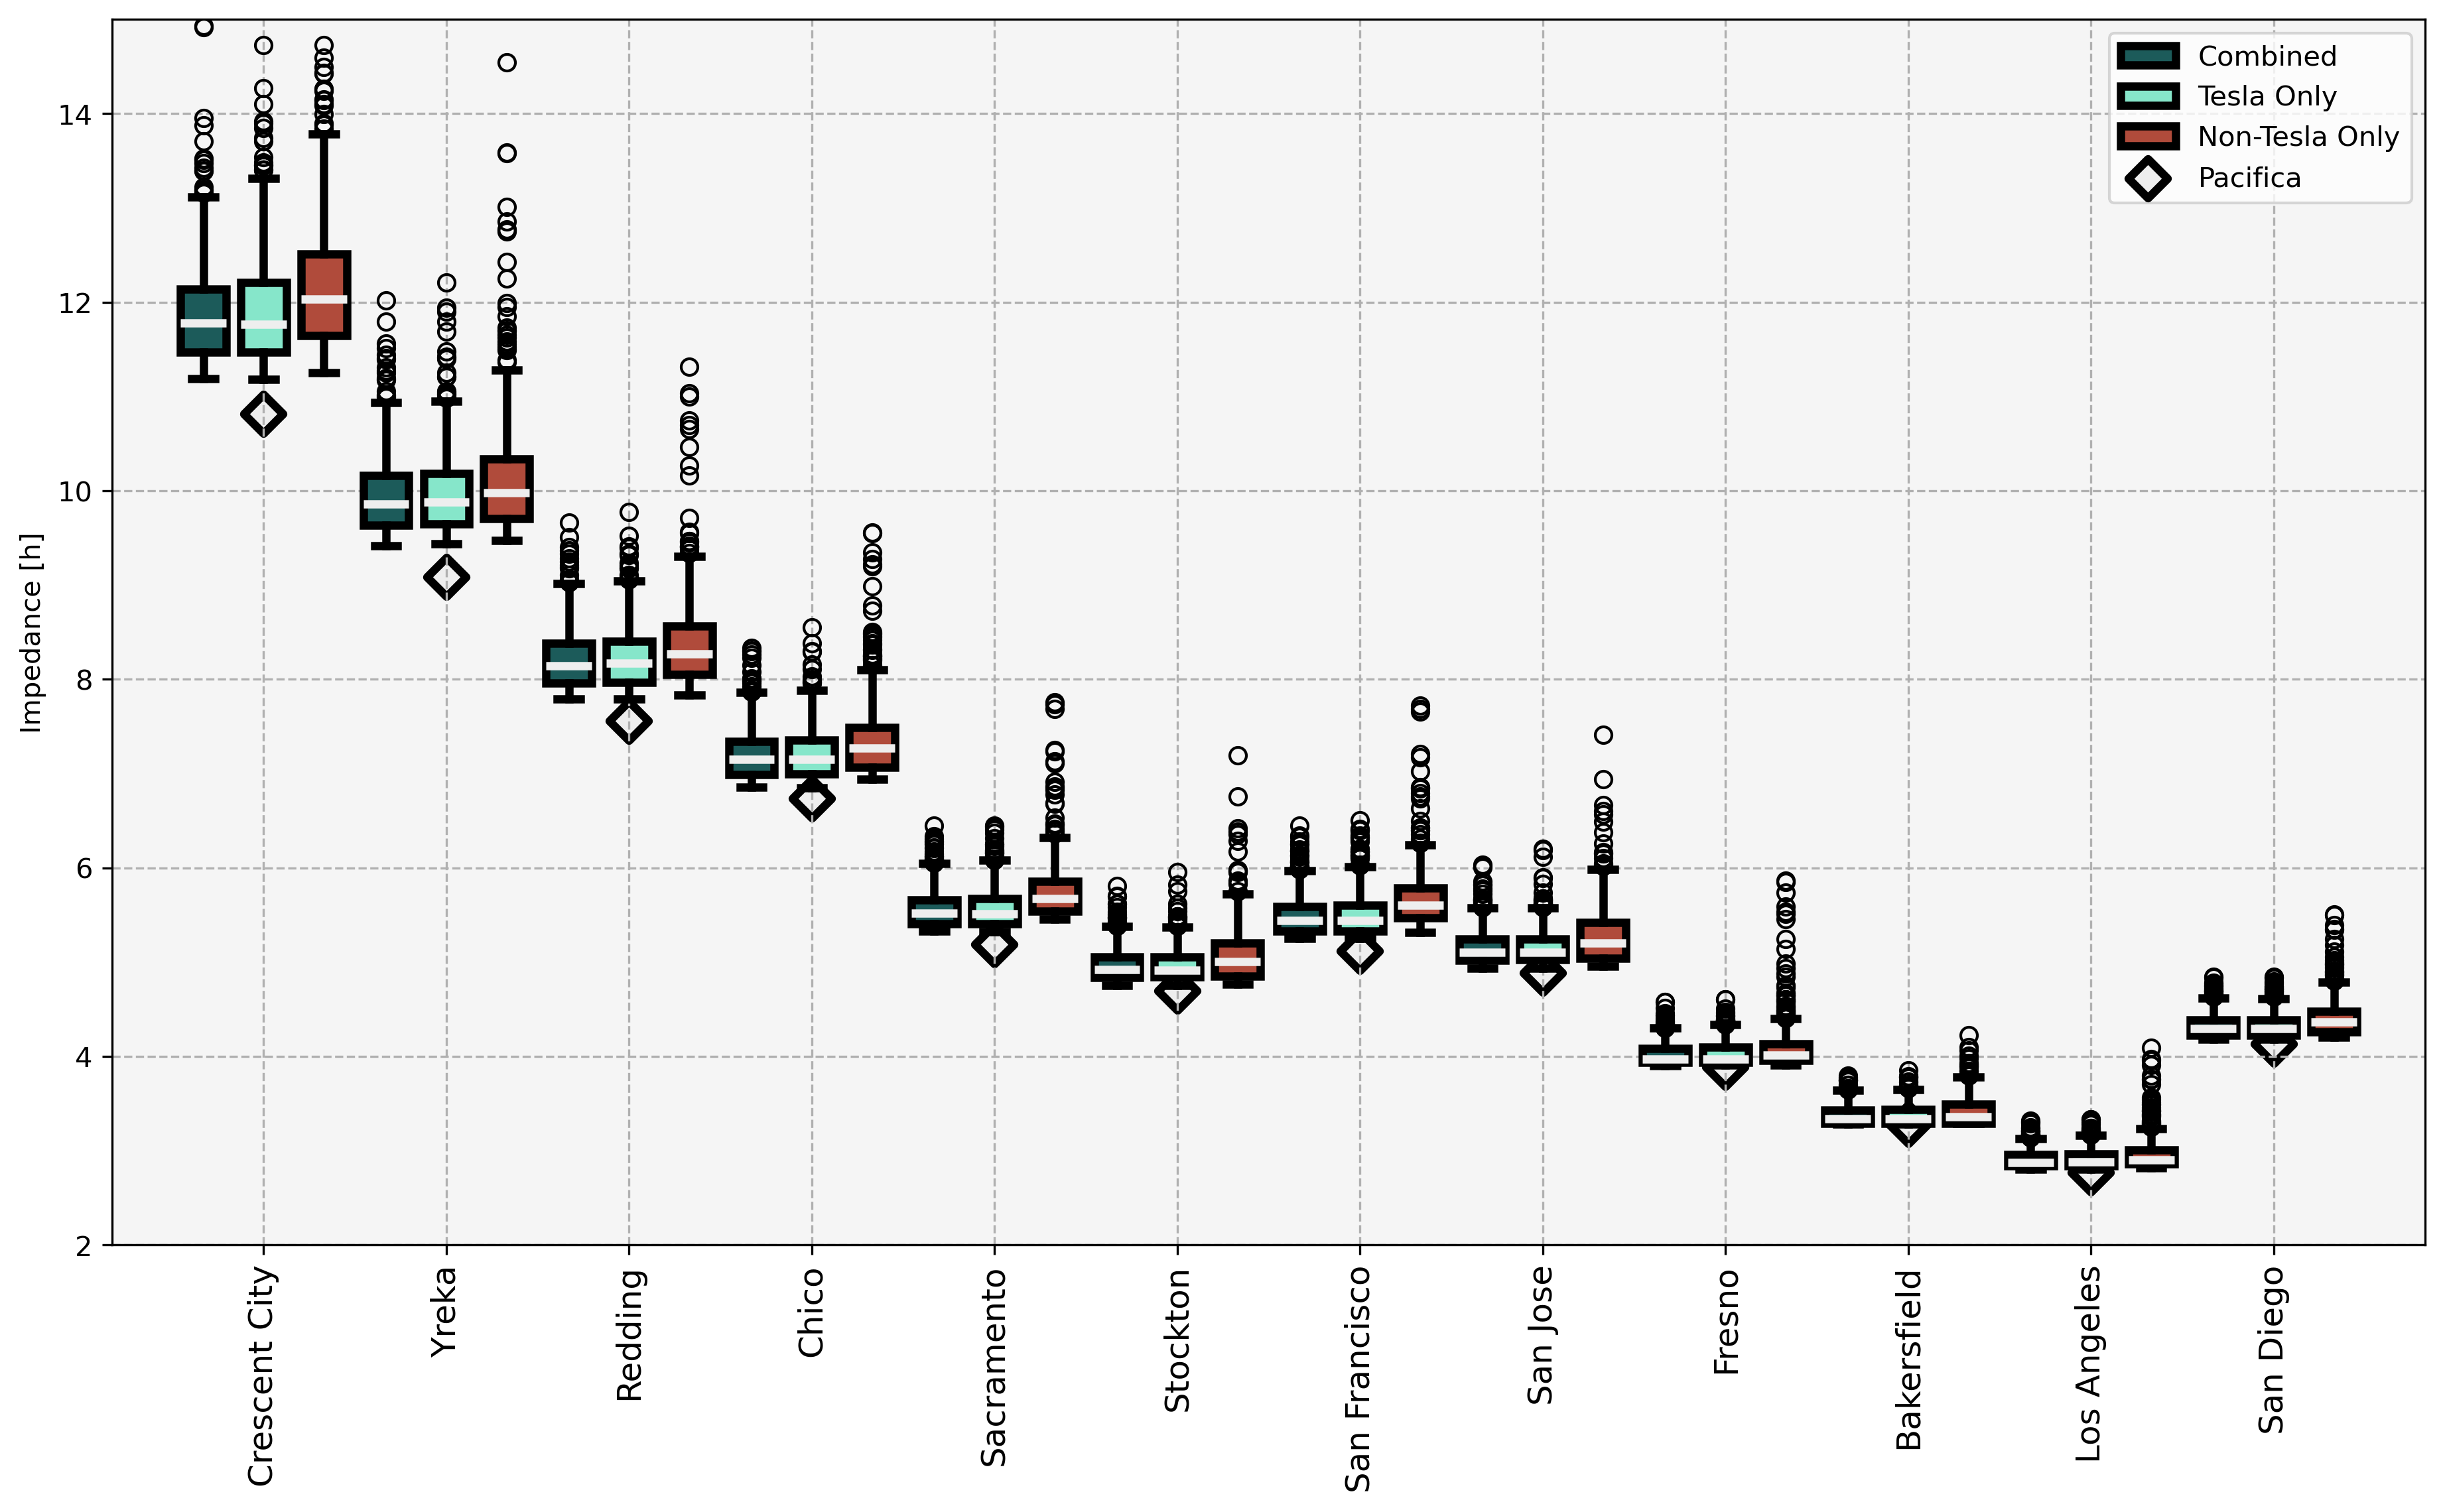
\includegraphics[width = \linewidth]{figs/Networks_Boxplots_Weighted_Specific_Impedance_2.png}
\caption{Boxplots of experiment outputs on combined \gls{sng} for each origin in California}
\label{fig:networks_boxplots_locations}
\end{figure}

\begin{multicols}{2}
	
\section*{Discussion}

The optimal routes generated in this study only selected corridor chargers. Some insight into the utility provided by each network can be gained by looking into utilization rates for networks and stations when using the combined \gls{sng}. Ratio of stations utilized at least once to total corridor stations in the combined \gls{sng} for each network is shown in Figure \ref{fig:utilization_rates}. Log of utilization (number of times utilized in random experiment) for corridor stations in the combined \gls{sng} is displayed in Figure \ref{fig:utilized_stations}.

\begin{figure}[H]
	\centering
	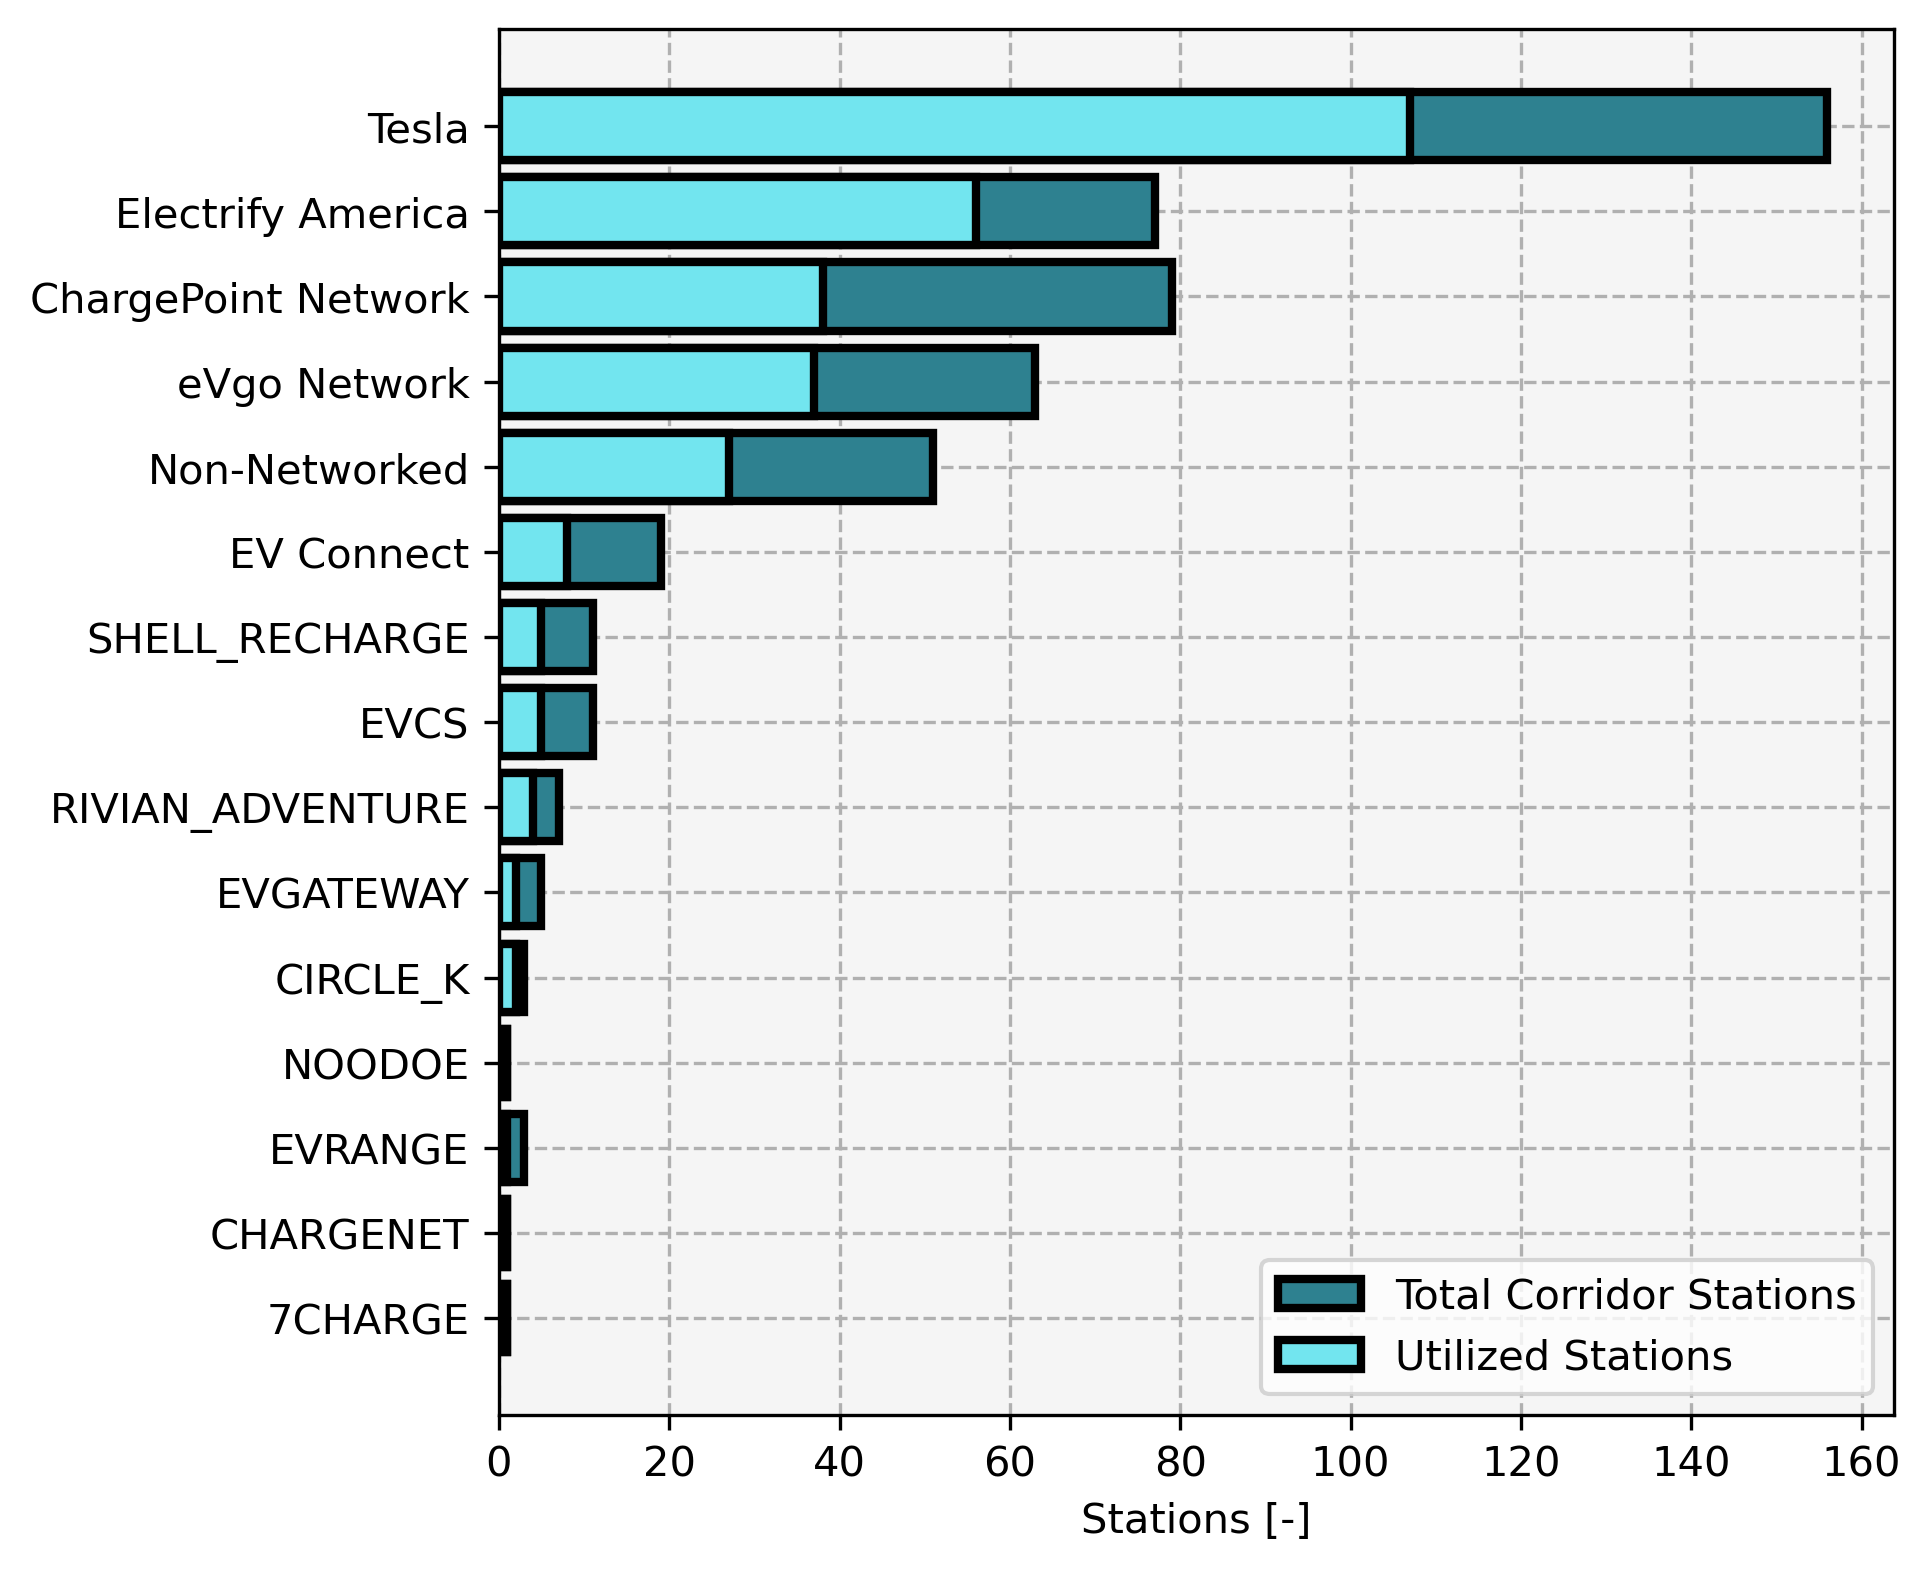
\includegraphics[width = \linewidth]{figs/corridor_station_utilization.png}
	\caption{Corridor DC charging network utilization rates}
	\label{fig:utilization_rates}
\end{figure}

\begin{figure}[H]
	\centering
	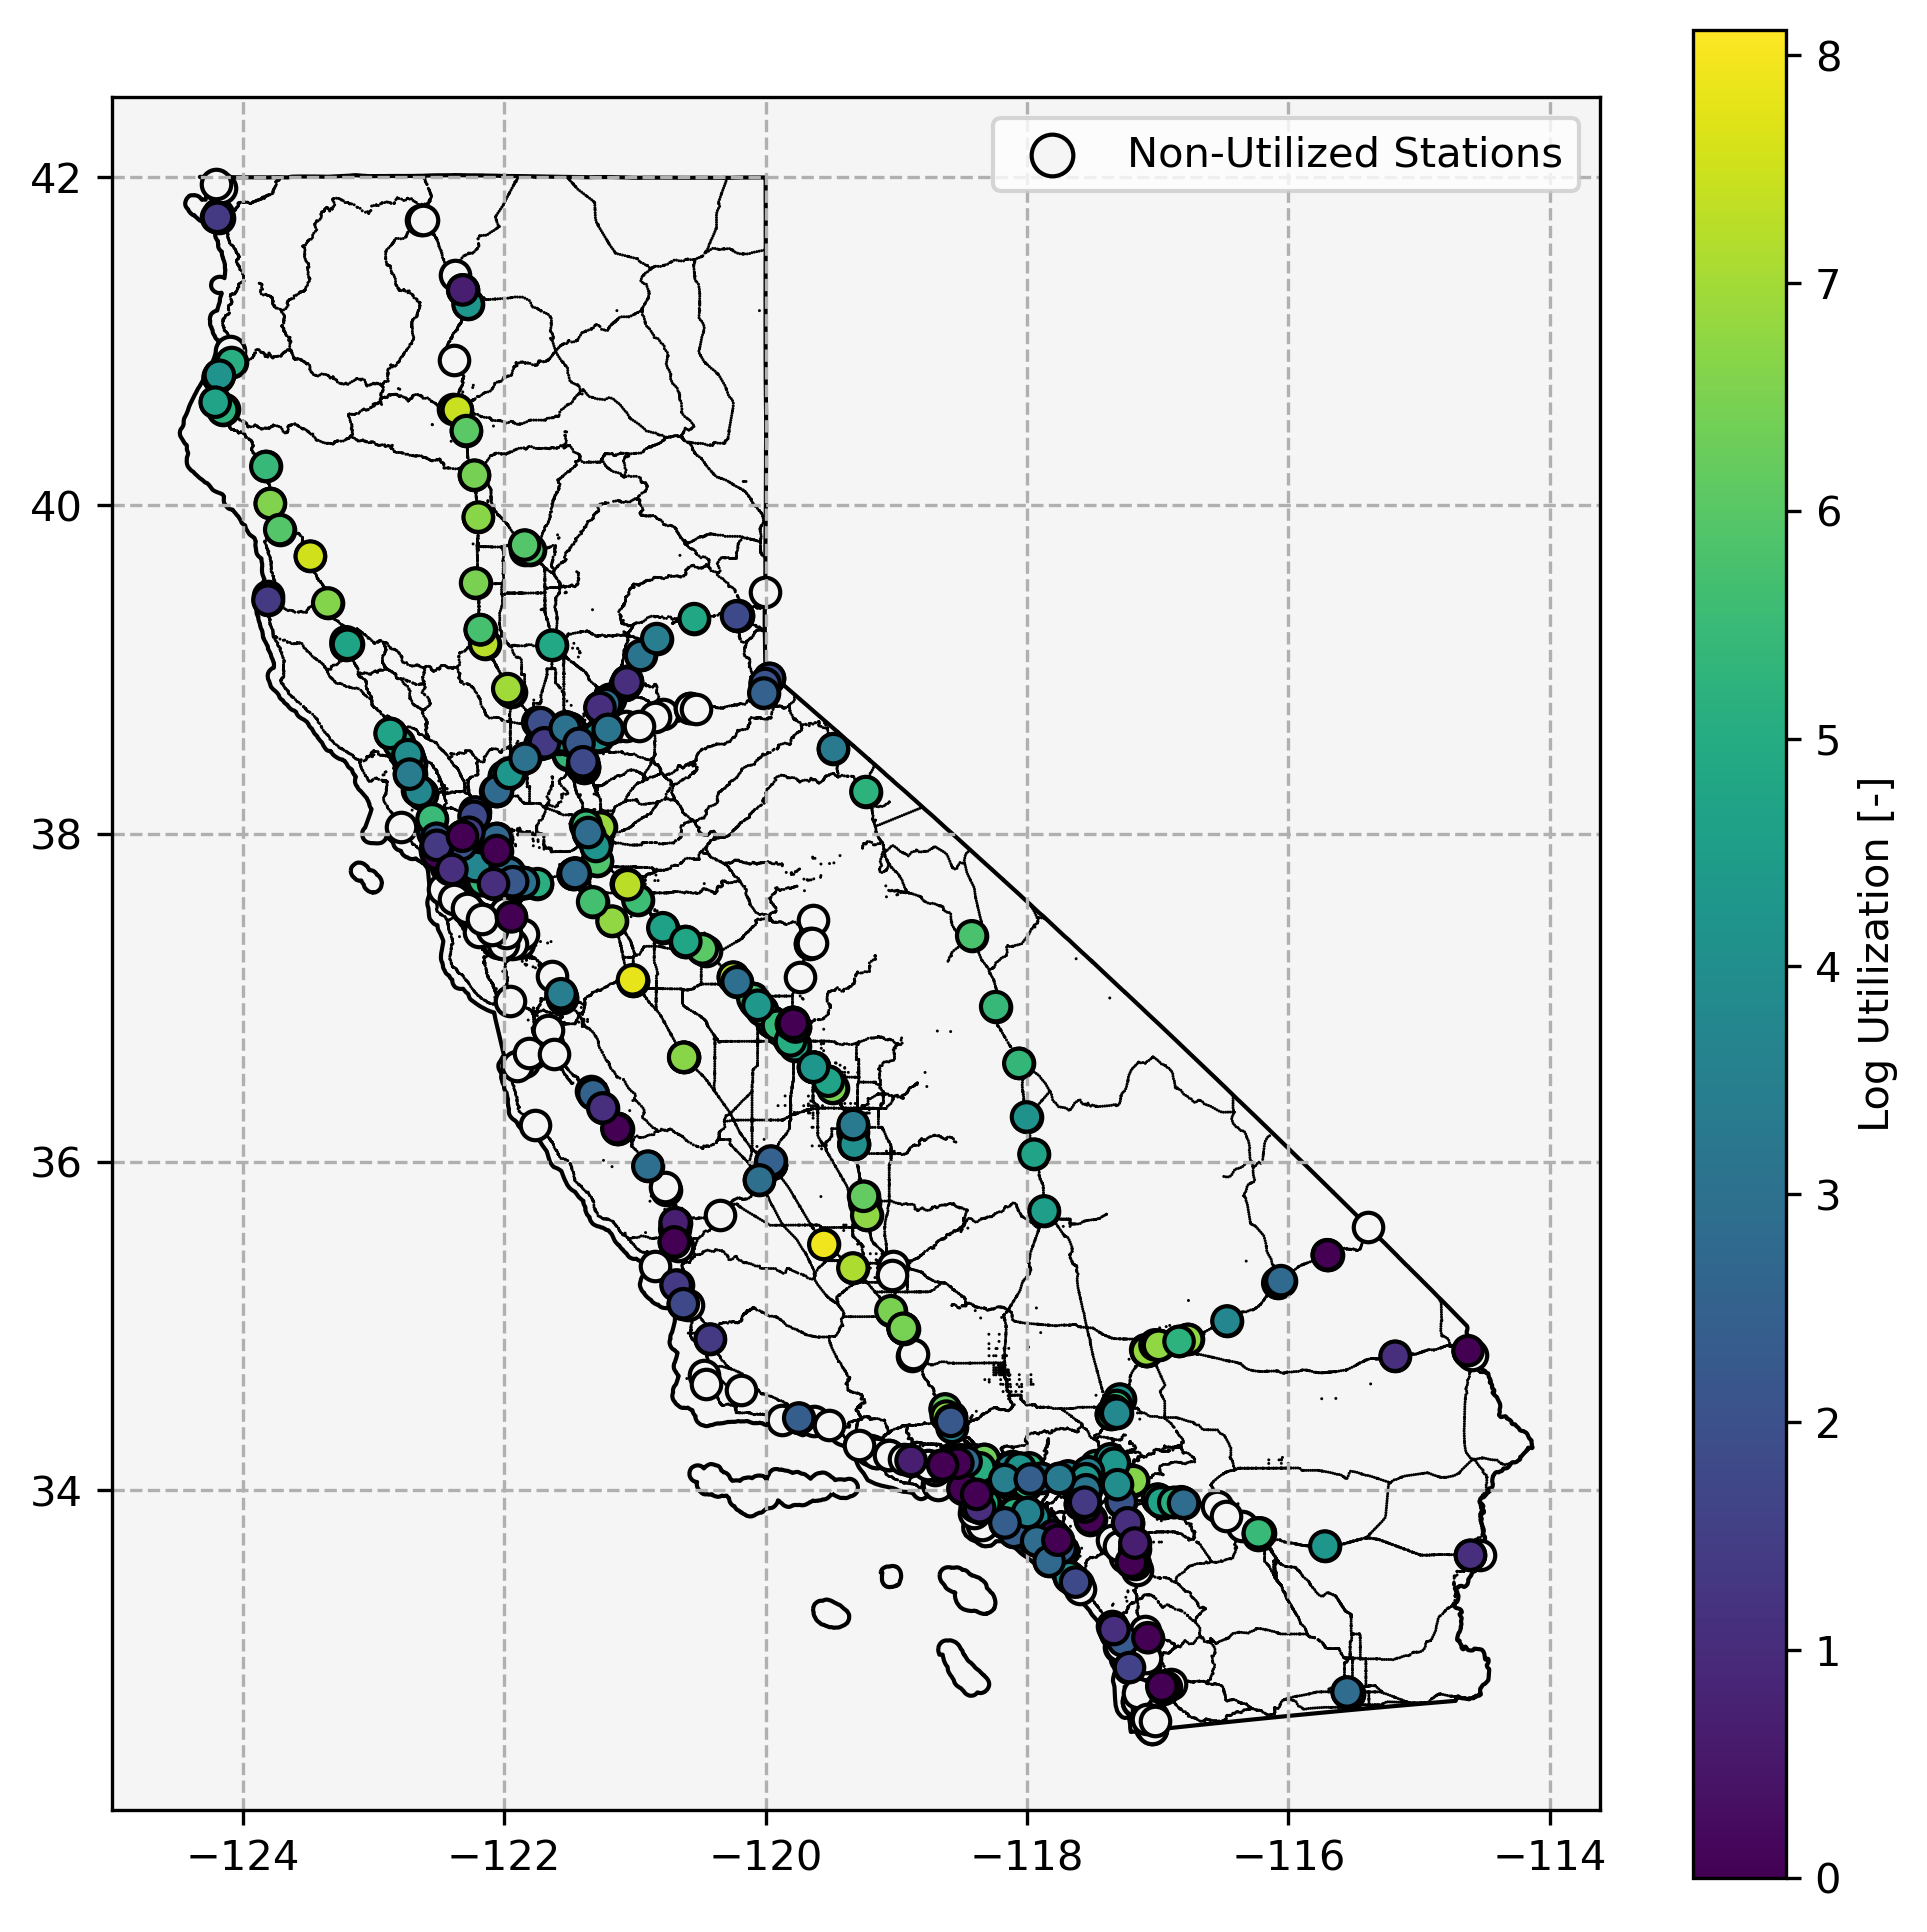
\includegraphics[width = \linewidth]{figs/California_SNG_Utilization.png}
	\caption{Corridor DC charging station log utilization}
	\label{fig:utilized_stations}
\end{figure}

It follows intuition that those chargers most useful for drivers are those located between cities on busy transportation corridors and this is backed up in this study. It also follows intuition that those chargers most likely to see use are those with higher redundancy in-station and lower redundancy in-corridor. In this sense Tesla stations are well positioned to absorb traffic should they become fully open to the general light duty \gls{ev} fleet. When one single entity has control over the locations of all stations in a network, that entity can concentrate chargers to maximize in-station redundancy and minimize between-station redundancy. That entity can, then strategically locate the highly concentrated stations. The result should be a network which experiences high utilization at each station and can benefit from economies of scale. When each network is developed by an independent actor these actors must build out their networks under the fear that a competitor could build a competing station near any of their stations at any time. The risk of building a large station only to lose business to a nearby competitor combined with the opportunity cost of not using limited capital to do the same inevitably results in a more inefficient combined network. However, many of the issues inherent with the distributed structure could be mitigated if the uncertainty and latency issues inherent to such a network could be mitigated. These issues can, possibly, be mitigated by an integrated status reporting and reservation system.


Often, the case for \glspl{bev} is made on an economic basis as \gls{bev} may have lower levelized costs of driving. This study focuses on travel times and routing did not optimize for cost. Partly, this is because at present there is no publicly available data on energy costs at a granular station-level for either gasoline or DC fast charging stations. Nevertheless, some sense of the relative economics of long-trip travel can be attained by examining energy costs per km. Energy costs vary substantially by region in the US with California being the most expensive. Energy costs around the time of writing are shown in Table \ref{tab:energy_costs}.

\begin{table}[H]
	\centering
	\caption{Residential electricity and petroleum average prices USD}
	\label{tab:energy_costs}
	\begin{tabular}{|C{.31\linewidth}|C{.23\linewidth}|C{.23\linewidth}|C{.23\linewidth}|}
		\hline Source & US & California & Percentage Increase \\
		\hline Petroleum [gallon] & 3.609 & 5.138 & 42.37 \\
		\hline Residential Electricity [kWh] & 0.1668 & 0.3247 & 94.66 \\
		\hline Transportation Electricity [kWh] & 0.1520 & 0.1191 & 27.62 \\
		\hline DC Fast Charging (Estimated) [kWh] & 0.35 - 0.50 & 0.35 - 0.60 & 0 - 20 \\
		\hline
	\end{tabular}
\end{table}

Petroleum prices are from AAA \cite{AAA_2024} and electricity prices are from EIA \cite{EIA_2024}. DC fast charging pricing schemes display much heterogeneity and may not be as easily accounted as metered electricity prices. An Ad-Hoc Text Mining study performed on over 90,000 recorded PlugShare events from 2019 and 2021 found the mode of DC fast charging prices to be in the range of 0.3 and 0.4 USD per kWh \cite{Trinko_2021}. Prices did not significantly correlate with local energy prices. In the same time period California residential electricity increased from 0.1995 USD per kWh to 0.2282 USD per kWh and transportation electricity increased from 0.0891 to 0.1179 USD per kWh. By comparison with 2024 electricity prices, one would expect prices in the range of 0.35 and 0.60 USD per kWh for DC fast charging in California and 0.35 to 0.5 in the US, ranges backed by informal reporting \cite{CalTrans_2024, Sowder_2024}. Thus, expected energy costs per highway km traveled can be computed and are shown in Table \ref{tab:expected_energy_costs_per_km}.

\begin{table}[H]
	\centering
	\caption{Expected energy costs per highway km traveled in US cents.}
	\label{tab:expected_energy_costs_per_km}
	\begin{tabular}{|C{\linewidth / 4}|C{\linewidth / 4}|C{\linewidth / 4}|C{\linewidth / 4}|}
		\hline Vehicle & Source & US Price & CA Price \\
		\hline Prius & Petroleum & 4.00 & 5.70 \\
		\hline Golf & Petroleum & 5.47 & 7.78 \\
		\hline Pacifica & Petroleum & 8.97 & 12.77 \\
		\hline \gls{bev} & Residential Electricity & 2.82 & 5.48 \\
		\hline \gls{bev} & DC Fast Charging & 5.91 - 8.44 & 5.91 - 10.13 \\
		\hline
	\end{tabular}
\end{table}

In the US, DC fast charging a \gls{bev} presents no appreciable economic benefit over fueling an efficient \gls{icev}. In much of the US, home-charging a \gls{bev} provides cost savings for daily travel and the initial part of a long trip. This is not the case in California where residential electricity is, on average, nearly twice as expensive as in the US as a whole.

If \glspl{bev} are a worse option than efficient \glspl{icev} for long trips on a time basis and no better on an energy cost basis this will make them less appealing to customers who value the ability to make long road trips. That customers seem to so highly value these uncommon events is a continuing source of frustration for \gls{bev} advocates. Negative perceptions of \gls{bev} long trip utility on consumer stated preference were found to be quite important in the late 2010s \cite{Skippon_2016, Hardman_2016, Franke_2017, Schmalfuss_2017}. In the intervening time period \gls{bev} ranges and maximum charge rates have markedly increased. Nevertheless, negative perceptions related to long trip utility persist for purchasers \cite{Bhat_2022, Paradies_2023, Corradi_2023, Philip_2023} and \gls{bev} range is a significant factor in determining usage share of \glspl{bev} in multi-vehicle household fleets \cite{Chakraborty_2022}. In the same time period, a massive build-out of DC charging infrastructure has taken place yet is not evident that the increased presence of DC charging infrastructure changes perceptions \cite{Hoogland_2023}.

As shown in Figure \ref{fig:utility_factors}, a \gls{bev} with 300 km of range can accomplish 80\% of US daily itineraries on a single charge. Fundamentally, the reality is that home or work charging leads to operational costs that often cheaper and rarely more expensive than petroleum. Similarly, home and work charging can lead to convenience benefits for \glspl{bev} as compared to \glspl{icev} \cite{Rabinowitz_2023} as \glspl{icev} require trips and trip deviations to reach supply stations. In theory, the trade-off of lower cost routine travel for higher cost long-distance travel is one which works in favor of \glspl{bev}. This is the logic which underpins the "charging pyramid" model which places long dwell charging events at its base and corridor DC fast charging events at the top. This model is also, to some degree, self-reinforcing. Because \gls{bev} drivers prefer AC charging, DC charging infrastructure has limited revenue potential leading to lower network capacity. Lower network capacity, in turn, leads to the perception that the network is inadequate and should be avoided.

The charging pyramid implies a different way of thinking about the role of car travel as a subset an individual's travel needs. Personal travel is inherently multi-modal and, for many \gls{od} arcs and many individuals, the cost differential between different modes is within the threshold of disambiguation. The strengths and weaknesses of \glspl{bev} as compared to \glspl{icev} may shift more short trips away from local transit and towards cars while shifting more long trips away from cars to air travel and inter-city transit. \glspl{bev} will only be one part of future mobility, unable to meet transportation needs or environmental goals on their own. Investments in \gls{bev} corridor infrastructure should be considered alongside investments into other low carbon inter-city transit modes.

\section*{Conclusions}

\lipsum[67] 

\newpage

\printbibliography

\newpage
\appendix

\section*{Appendix}

\subsection*{DC Charger Network Details}

Network characteristics for DC charging networks in California are shown in Figure \ref{fig:ris_top_networks} and in Table \ref{tab:summary_statistics_afdc}. Data pulled from \gls{afdc} in May 2024.

\begin{figure}[H]
	\centering
	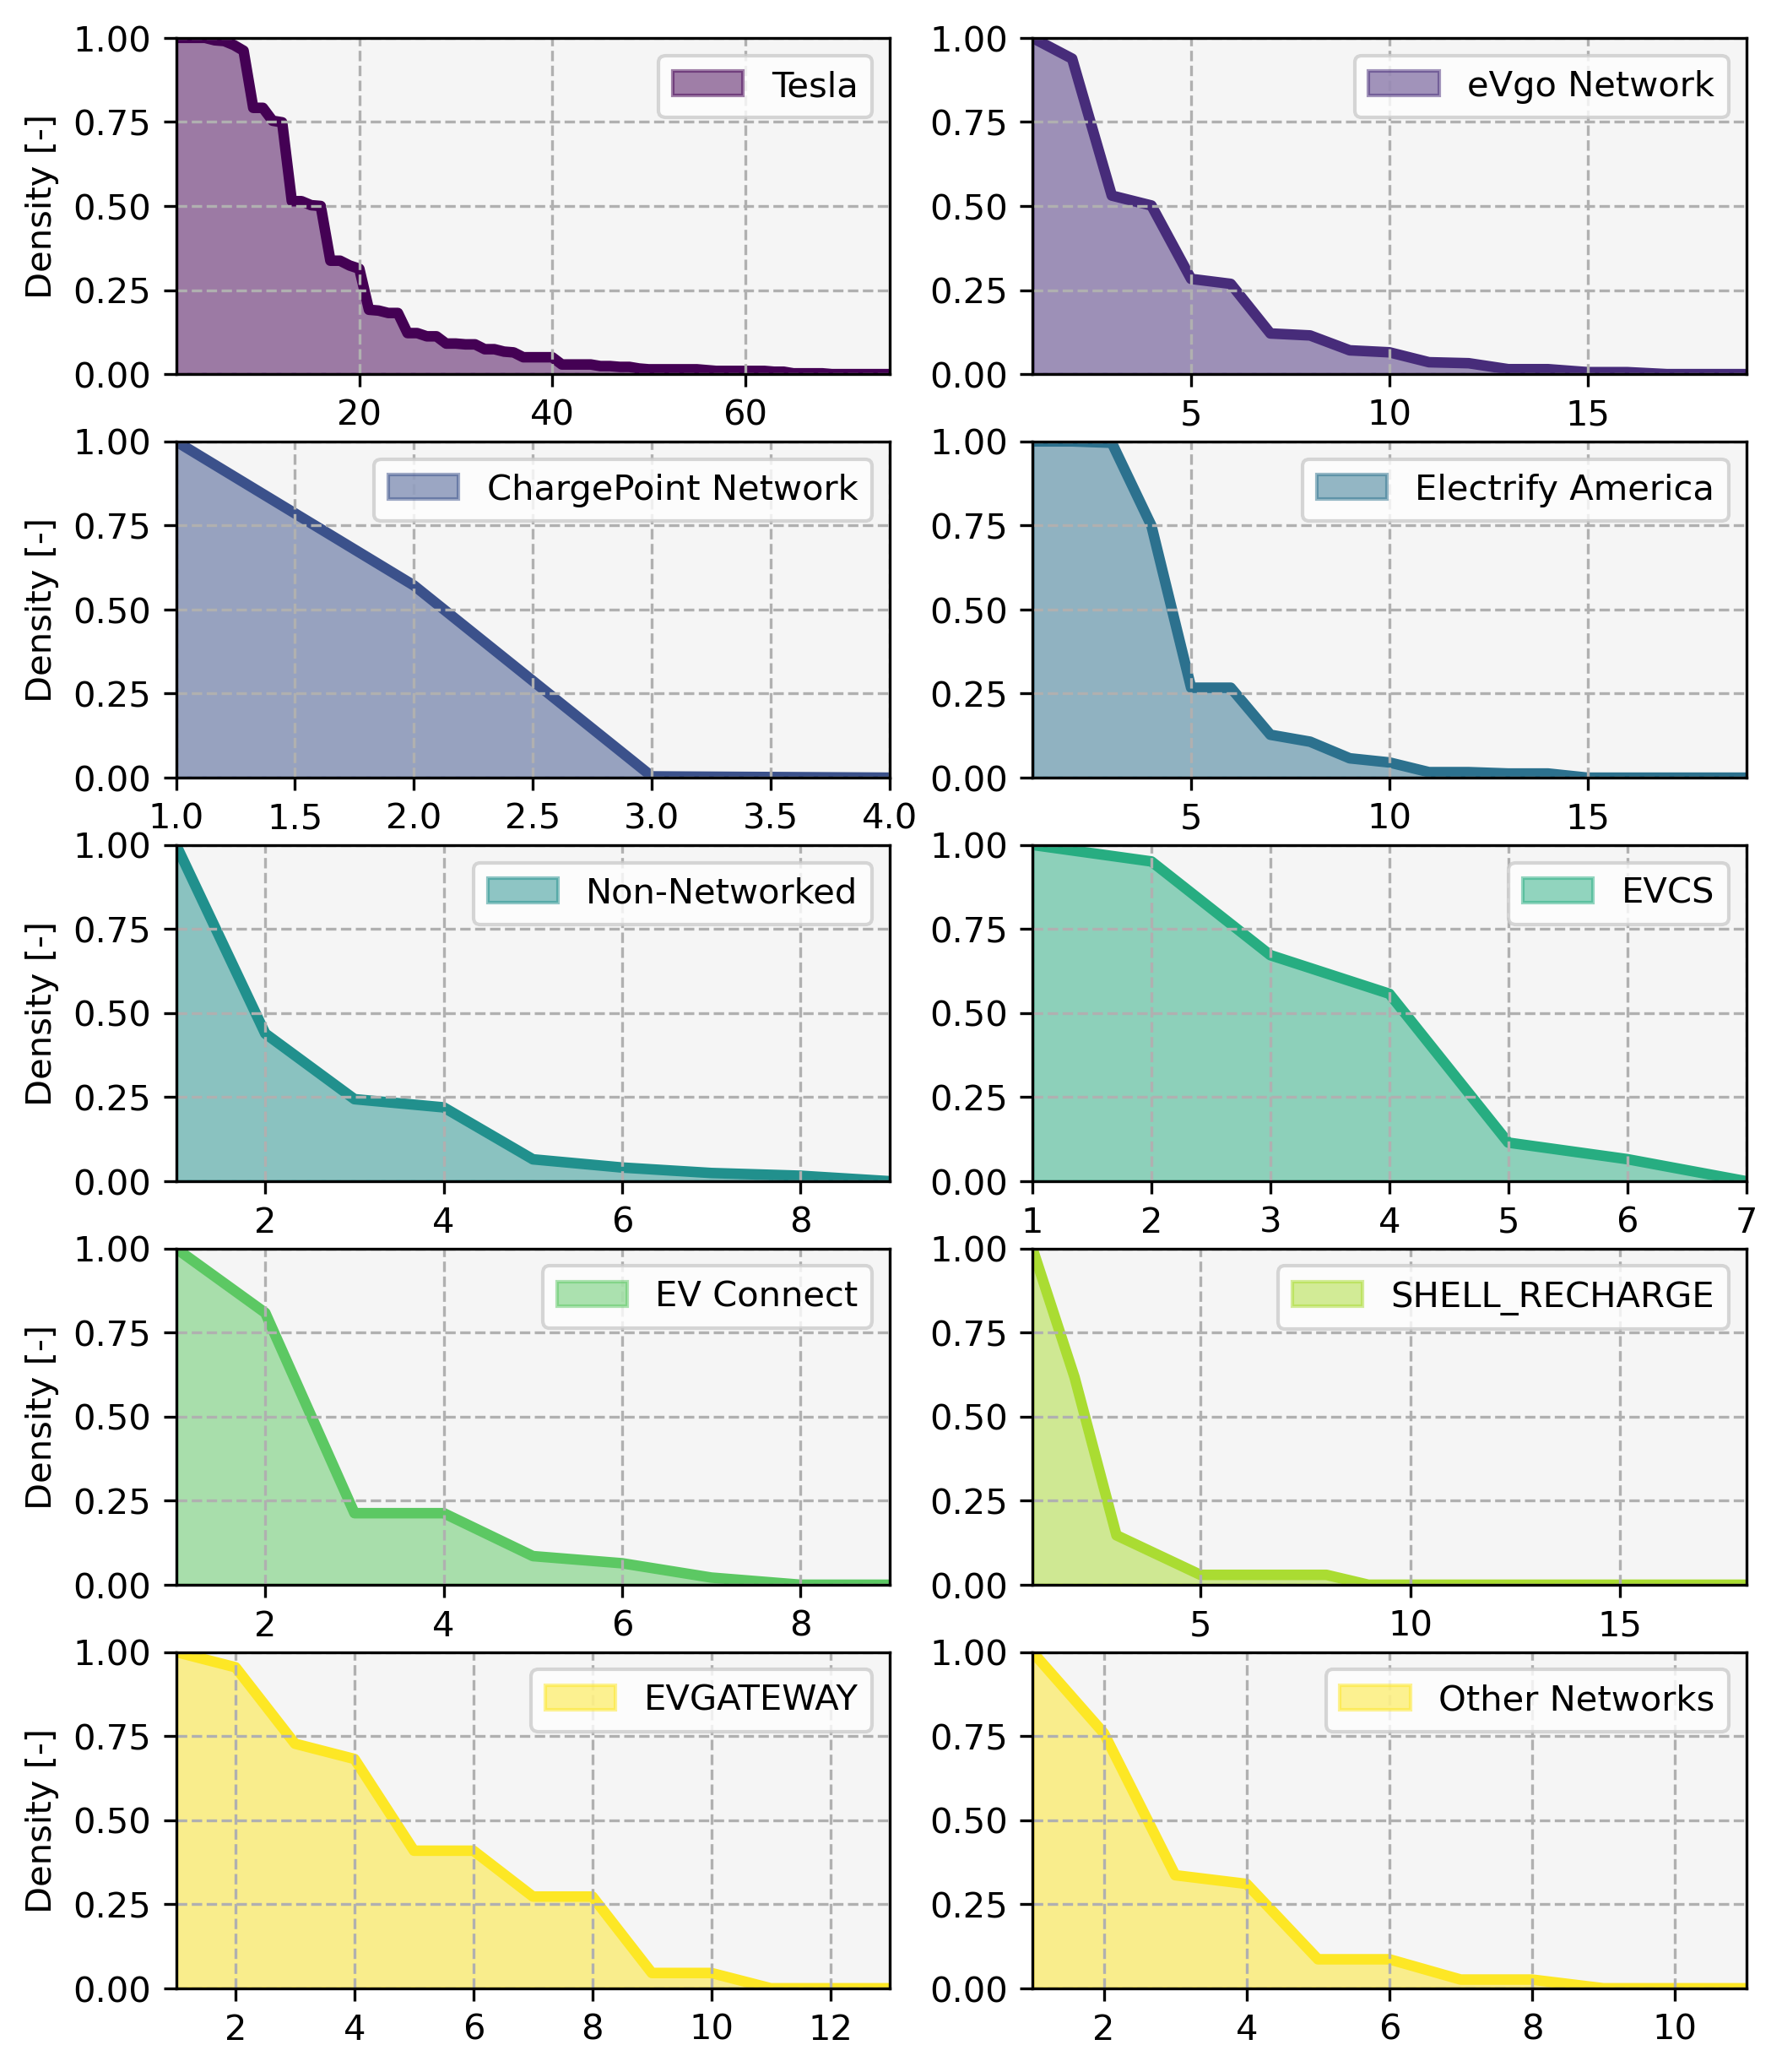
\includegraphics[width = \linewidth]{figs/California_RIS_SF_All.png}
	\caption{In-station redundancy for DC Charging networks in California}
	\label{fig:ris_top_networks}
\end{figure}

\begin{table}[H]
	\centering
	\caption{Summary statistics for California DC charging networks from \gls{afdc}}
	\label{tab:summary_statistics_afdc}
	\begin{tabular}{|C{.46\linewidth}|C{.18\linewidth}|C{.18\linewidth}|C{.18\linewidth}|}
		\hline Network & Chargers & Stations & Chargers per Station \\
		\hline Non-Networked & 288 & 51 & 5.6 \\
		\hline Tesla & 2753 & 156 & 17.6 \\
		\hline Electrify America & 526 & 77 & 6.8 \\
		\hline EV Connect & 59 & 19 & 3.1 \\
		\hline ChargePoint Network & 186 & 79 & 2.4 \\
		\hline Volta & 2 & 2 & 1.0 \\
		\hline EVCS & 41 & 11 & 3.7 \\
		\hline SHELL_RECHARGE & 39 & 11 & 3.5 \\
		\hline EVGATEWAY & 21 & 5 & 4.2 \\
		\hline eVgo Network & 332 & 63 & 5.3 \\
		\hline BP_PULSE & 3 & 2 & 1.5 \\
		\hline POWERFLEX & 12 & 3 & 4.0 \\
		\hline FLO & 1 & 1 & 1.0 \\
		\hline EVRANGE & 11 & 3 & 3.7 \\
		\hline RIVIAN_ADVENTURE & 14 & 7 & 2.0 \\
		\hline CIRCLE_K & 16 & 3 & 5.3 \\
		\hline CHARGENET & 7 & 1 & 7.0 \\
		\hline Blink Network & 2 & 2 & 1.0 \\
		\hline NOODOE & 2 & 1 & 2.0 \\
		\hline LOOP & 6 & 2 & 3.0 \\
		\hline 7CHARGE & 4 & 1 & 4.0 \\
		\hline
	\end{tabular}
\end{table}

Network characteristics for DC charging networks in California, conunting only corridor chargers, are shown in Figure \ref{fig:ris_top_networks} and in Table \ref{tab:summary_statistics_afdc}. Data pulled from \gls{afdc} in May 2024.

\begin{figure}[H]
	\centering
	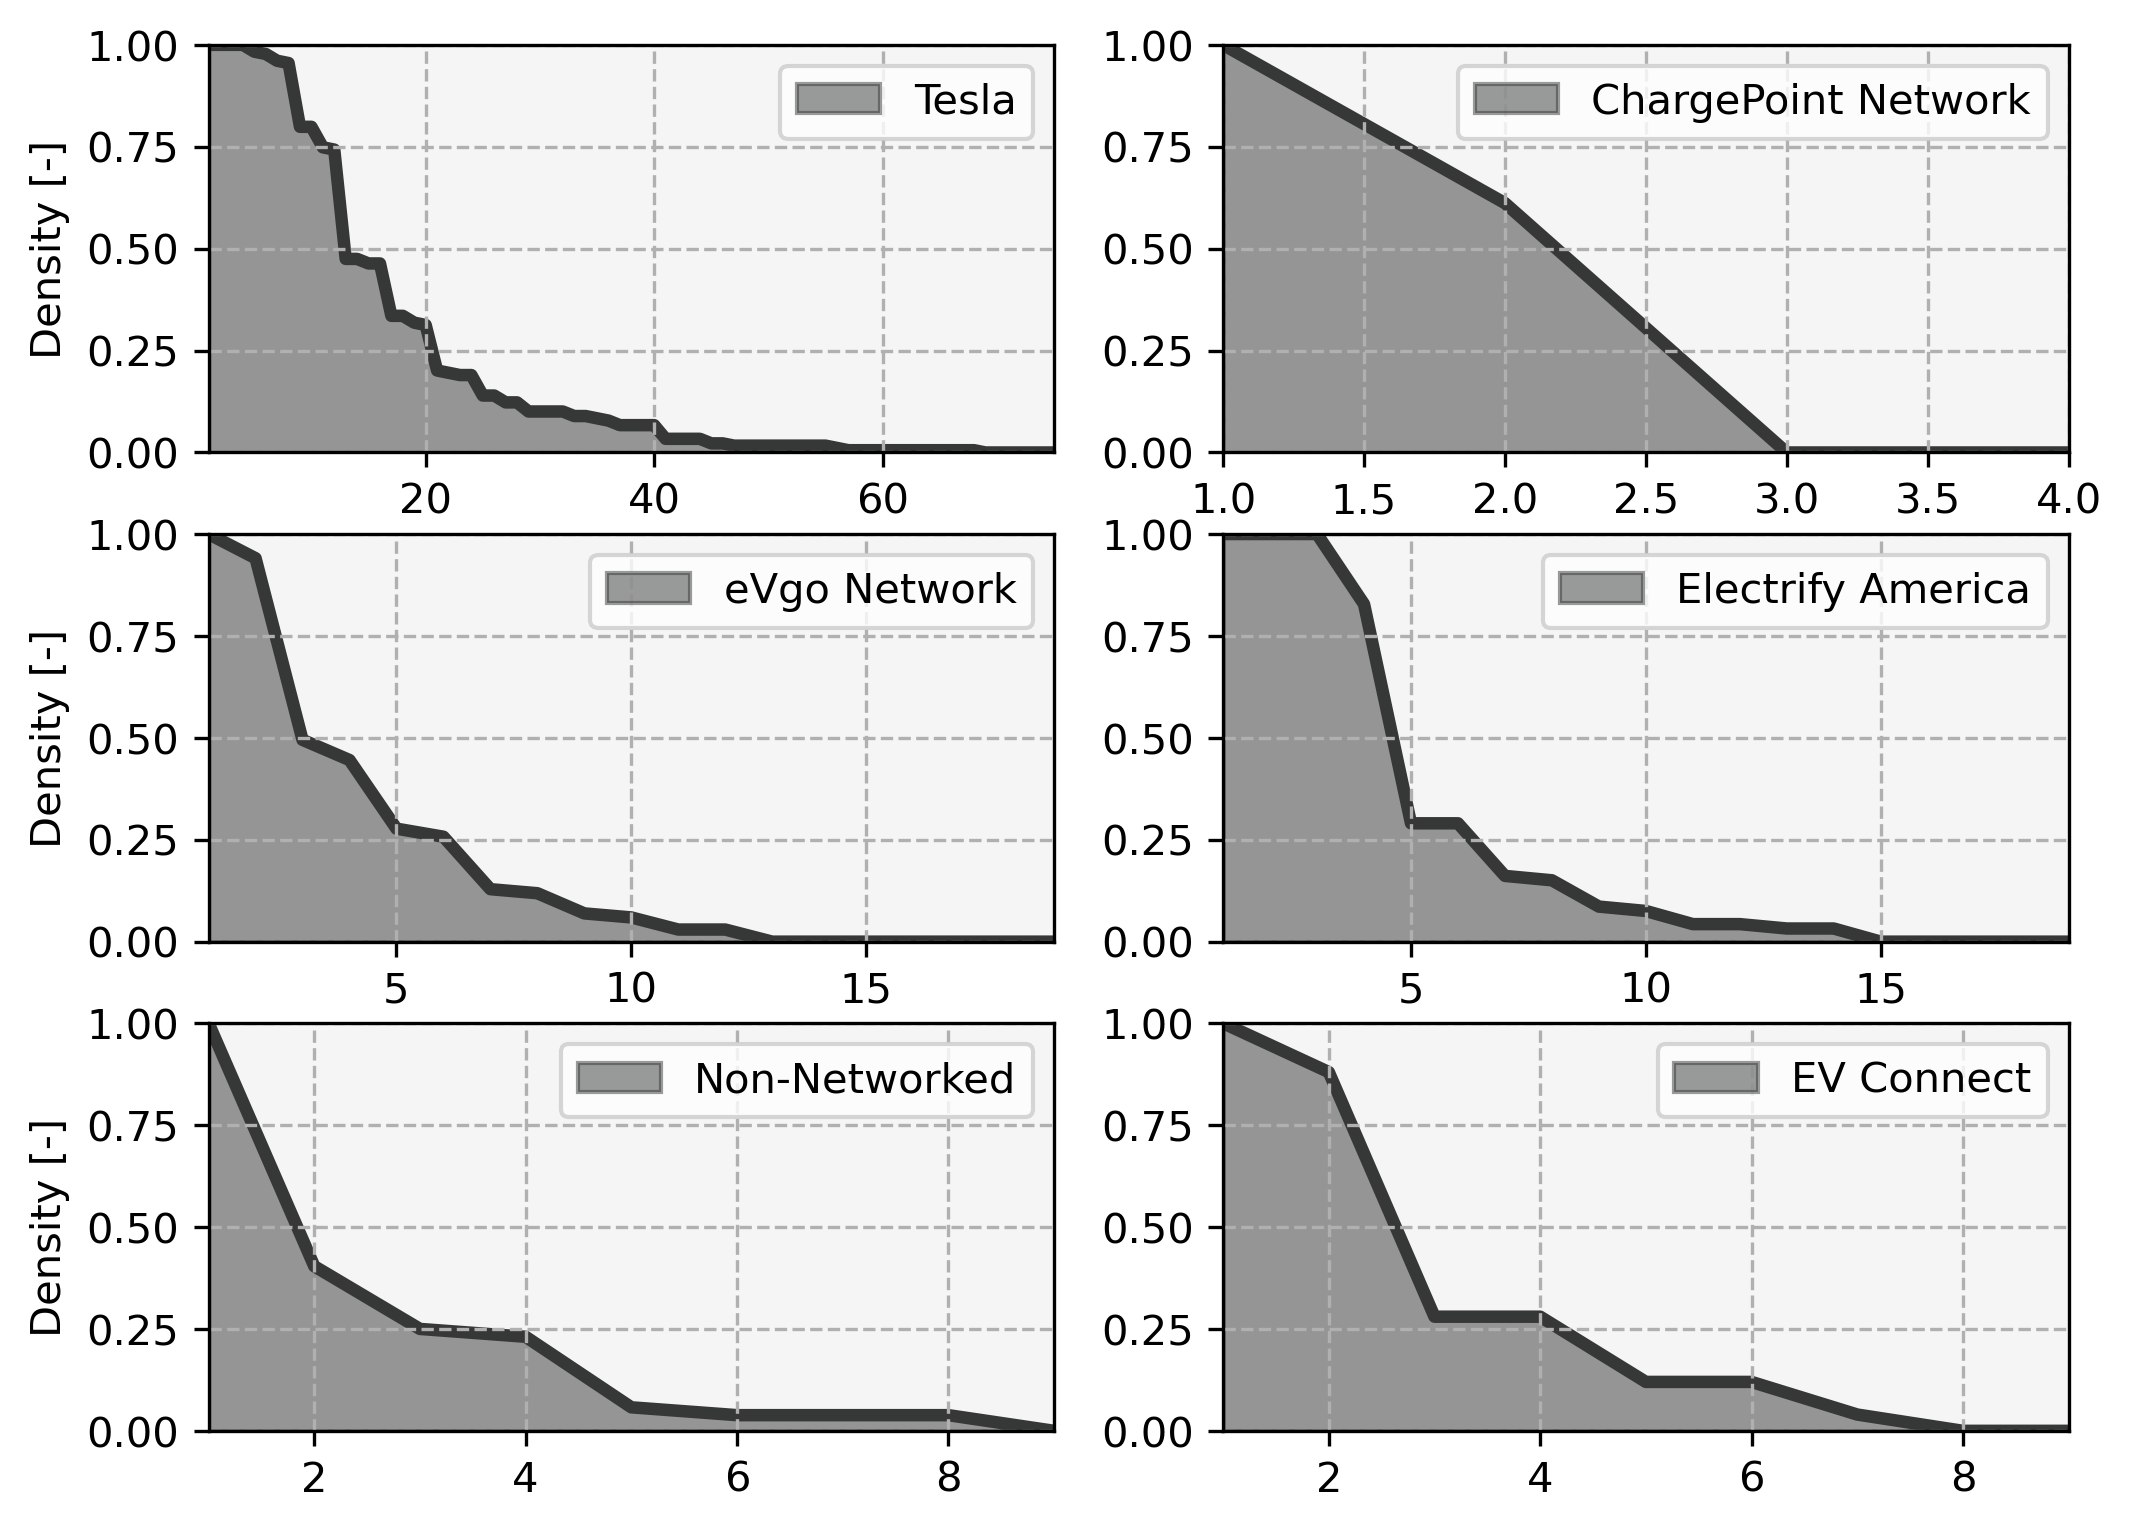
\includegraphics[width = \linewidth]{figs/California_RIS_SF_Corridor.png}
	\caption{In-station redundancy for DC Charging networks in California}
	\label{fig:ris_top_networks_corridor}
\end{figure}

\begin{table}[H]
	\centering
	\caption{Summary statistics for California DC charging networks from \gls{afdc} (corridor stations)}
	\label{tab:summary_statistics_afdc_corridor}
	\begin{tabular}{|C{.46\linewidth}|C{.18\linewidth}|C{.18\linewidth}|C{.18\linewidth}|}
		\hline Network & Chargers & Stations & Chargers per Station \\
		\hline Non-Networked & 274 & 50 & 5.5 \\
		\hline Tesla & 2745 & 155 & 17.7 \\
		\hline Electrify America & 518 & 76 & 6.8 \\
		\hline EV Connect & 58 & 18 & 3.2 \\
		\hline ChargePoint Network & 184 & 78 & 2.4 \\
		\hline Volta & 1 & 1 & 1.0 \\
		\hline EVCS & 35 & 10 & 3.5 \\
		\hline SHELL_RECHARGE & 37 & 10 & 3.7 \\
		\hline EVGATEWAY & 19 & 4 & 4.8 \\
		\hline eVgo Network & 329 & 62 & 5.3 \\
		\hline BP_PULSE & 1 & 1 & 1.0 \\
		\hline POWERFLEX & 10 & 2 & 5.0 \\
		\hline EVRANGE & 5 & 2 & 2.5 \\
		\hline RIVIAN_ADVENTURE & 12 & 6 & 2.0 \\
		\hline CIRCLE_K & 12 & 2 & 6.0 \\
		\hline Blink Network & 1 & 1 & 1.0 \\
		\hline LOOP & 2 & 1 & 2.0 \\
		\hline
	\end{tabular}
\end{table}

\subsection*{Regression Details}

Details of linear regression on random experiment results are displayed in the following tables. Tables \ref{tab:regression_anova_c} and \ref{tab:regression_coefficients_c} concern the combined network, Tables \ref{tab:regression_anova_t} and \ref{tab:regression_coefficients_t} concern the Tela network, and Tables \ref{tab:regression_anova_nt} and \ref{tab:regression_coefficients_nt} concern the non-Tesla network.

\begin{table}[H]
	\centering
	\caption{Combined Network Linear Regression Analysis ANOVA}
	\label{tab:regression_anova_c}
	\begin{tabular}{|C{.25\linewidth}|C{.25\linewidth}|C{.25\linewidth}|C{.25\linewidth}|}
		\hline \rowcolor{lightgray} R & R-Squared & Adjusted R-Squared & Std. Error \\
		\hline 0.926 & 0.858 & 0.853 & 0.000 \\
		\hline \rowcolor{lightgray} Category & Sum of Squares & DOF & Mean Squares \\
		\hline Model & 28.706 & 15 & 1.914 \\
		\hline Error & 4.754 & 484 & 0.010 \\
		\hline Total & 33.460 & 499 & 0.067 \\
		\hline  \rowcolor{lightgray} \multicolumn{2}{|c|}{$F$} &  \multicolumn{2}{c|}{$P(>F)$}  \\
		\hline  \multicolumn{2}{|c|}{194.848} &  \multicolumn{2}{c|}{0.000}  \\
		\hline
	\end{tabular}
\end{table}

\begin{table}[H]
	\centering
	\caption{Combined Network Linear Regression Analysis Significant Coefficients ($\alpha = 0.5$)}
	\label{tab:regression_coefficients_c}
	\begin{tabular}{|C{.5\linewidth}|C{.25\linewidth}|C{.25\linewidth}|}
		\hline \rowcolor{lightgray} Parameter & Coefficient & P-Value \\
		\hline {\small Intercept } & 7.121 & 0.000 \\
		\hline {\small power } & -1.009 & 0.000 \\
		\hline {\small capacity } & -1.031 & 0.000 \\
		\hline {\small reliability } & -0.227 & 0.040 \\
		\hline {\small capacity:power } & 0.984 & 0.000 \\
		\hline {\small capacity:reliability } & 0.422 & 0.036 \\
		\hline
	\end{tabular}
\end{table}

\begin{table}[H]
	\centering
	\caption{Tesla Network Linear Regression Analysis ANOVA}
	\label{tab:regression_anova_t}
	\begin{tabular}{|C{.25\linewidth}|C{.25\linewidth}|C{.25\linewidth}|C{.25\linewidth}|}
		\hline \rowcolor{lightgray} R & R-Squared & Adjusted R-Squared & Std. Error \\
		\hline 0.926 & 0.857 & 0.852 & 0.000 \\
		\hline \rowcolor{lightgray} Category & Sum of Squares & DOF & Mean Squares \\
		\hline Model & 27.188 & 15 & 1.813 \\
		\hline Error & 4.541 & 480 & 0.009 \\
		\hline Total & 31.728 & 495 & 0.064 \\
		\hline  \rowcolor{lightgray} \multicolumn{2}{|c|}{$F$} &  \multicolumn{2}{c|}{$P(>F)$}  \\
		\hline  \multicolumn{2}{|c|}{191.609} &  \multicolumn{2}{c|}{0.000}  \\
		\hline
	\end{tabular}
\end{table}

\begin{table}[H]
	\centering
	\caption{Tesla Network Linear Regression Analysis Significant Coefficients ($\alpha = 0.5$)}
	\label{tab:regression_coefficients_t}
	\begin{tabular}{|C{.5\linewidth}|C{.25\linewidth}|C{.25\linewidth}|}
		\hline \rowcolor{lightgray} Parameter & Coefficient & P-Value \\
		\hline {\small Intercept } & 7.218 & 0.000 \\
		\hline {\small power } & -1.099 & 0.000 \\
		\hline {\small capacity } & -1.179 & 0.000 \\
		\hline {\small reliability } & -0.220 & 0.047 \\
		\hline {\small capacity:power } & 1.130 & 0.000 \\
		\hline {\small power:risk_attitude } & 0.479 & 0.035 \\
		\hline {\small capacity:reliability } & 0.481 & 0.016 \\
		\hline {\small capacity:power:risk_attitude } & -0.879 & 0.028 \\
		\hline
	\end{tabular}
\end{table}

\begin{table}[H]
	\centering
	\caption{Non-Tesla Network Linear Regression Analysis ANOVA}
	\label{tab:regression_anova_nt}
	\begin{tabular}{|C{.25\linewidth}|C{.25\linewidth}|C{.25\linewidth}|C{.25\linewidth}|}
		\hline R & R-Squared & Adjusted R-Squared & Std. Error \\
		\hline 0.866 & 0.750 & 0.742 & 0.000 \\
		\hline
		\hline Category & Sum of Squares & DOF & Mean Squares \\
		\hline Model & 72.583 & 15 & 4.839 \\
		\hline Error & 24.215 & 484 & 0.050 \\
		\hline Total & 96.798 & 499 & 0.194 \\
		\hline  \multicolumn{2}{|c|}{$F$} &  \multicolumn{2}{c|}{$P(>F)$}  \\
		\hline  \multicolumn{2}{|c|}{96.720} &  \multicolumn{2}{c|}{0.000}  \\
		\hline
	\end{tabular}
\end{table}

\begin{table}[H]
	\centering
	\caption{Non-Tesla Network Linear Regression Analysis Coefficients}
	\label{tab:regression_coefficient_nt}
	\begin{tabular}{|C{.5\linewidth}|C{.25\linewidth}|C{.25\linewidth}|}
		\hline Parameter & Coefficient & P-Value \\
		\hline {\small Intercept } & 7.095 & 0.000 \\
		\hline {\small power } & -1.373 & 0.000 \\
		\hline {\small capacity } & -1.130 & 0.000 \\
		\hline {\small risk_attitude } & 0.954 & 0.001 \\
		\hline {\small capacity:power } & 1.505 & 0.004 \\
		\hline {\small power:risk_attitude } & 1.429 & 0.006 \\
		\hline {\small capacity:power:risk_attitude } & -1.915 & 0.037 \\
		\hline {\small power:reliability:risk_attitude } & -1.744 & 0.047 \\
		\hline
	\end{tabular}
\end{table}

\end{multicols}

\end{document}